% ------------------------------------------------------------------------
% MS Thesis of Juan de la Cruz
% Date Defended: May 31, 2000
% ------------------------------------------------------------------------
\documentclass[letterpaper,12pt]{report}
\usepackage[centertags]{amsmath}
\usepackage{algpseudocode}
\usepackage{algorithm}
\usepackage{amsfonts}
\usepackage{amssymb}
\usepackage{amsthm}
\usepackage{amsmath}
\usepackage{newlfont}
\usepackage{epsfig}
\usepackage{longtable}
\usepackage{UPCSTHESIS} %This loads the UP Computer Science Thesis Package
\usepackage{UPCSINC1}
\usepackage[active]{LTX}
\usepackage{subfig}
\usepackage{listings}
\usepackage{array}
\usepackage{graphicx}
\usepackage{float}
\usepackage{url}

\usepackage{fancyhdr}

\fancyhf{} % clear all header and footer fields
\fancyhead[R]{\thepage}

\renewcommand{\headrulewidth}{0pt}
\renewcommand{\footrulewidth}{0pt}

% Redefining plain style which is automatically applied to chapters (including Bibliography)

\fancypagestyle{plain}{%
\fancyhf{} % clear all header and footer fields
\fancyhead[R]{\thepage}
\renewcommand{\headrulewidth}{0pt}
\renewcommand{\footrulewidth}{0pt}}

\pagestyle{fancy} 

%% Define a new 'leo' style for the package that will use a smaller font.
\makeatletter
\def\url@leostyle{%
  \@ifundefined{selectfont}{\def\UrlFont{\sf}}{\def\UrlFont{\small\ttfamily}}}
\makeatother
%% Now actually use the newly defined style.
\urlstyle{leo}


\hfuzz2pt
\newlength{\defbaselineskip}
\setlength{\defbaselineskip}{\baselineskip}
\newcommand{\setlinespacing}[1]%
           {\setlength{\baselineskip}{#1 \defbaselineskip}}
\newcommand{\doublespacing}{\setlength{\baselineskip}%
                           {2.0 \defbaselineskip}}
\newcommand{\singlespacing}{\setlength{\baselineskip}{\defbaselineskip}}
% Algorithm Commands
\newcommand{\WRP}{\par\quad\(\hookrightarrow\)\enspace}

% MATH -------------------------------------------------------------------
\newcommand{\A}{{\cal A}}
\newcommand{\h}{{\cal H}}
\newcommand{\s}{{\cal S}}
\newcommand{\W}{{\cal W}}
\newcommand{\BH}{\mathbf B(\cal H)}
\newcommand{\KH}{\cal  K(\cal H)}
\newcommand{\Real}{\mathbb R}
\newcommand{\Complex}{\mathbb C}
\newcommand{\Field}{\mathbb F}
\newcommand{\RPlus}{[0,\infty)}
\newcommand{\norm}[1]{\left\Vert#1\right\Vert}
\newcommand{\essnorm}[1]{\norm{#1}_{\text{\rm\normalshape ess}}}
\newcommand{\abs}[1]{\left\vert#1\right\vert}
\newcommand{\set}[1]{\left\{#1\right\}}
\newcommand{\seq}[1]{\left<#1\right>}
\newcommand{\eps}{\varepsilon}
\newcommand{\To}{\longrightarrow}
\newcommand{\RE}{\operatorname{Re}}
\newcommand{\IM}{\operatorname{Im}}
\newcommand{\Poly}{{\cal{P}}(E)}
\newcommand{\EssD}{{\cal{D}}}
% THEOREMS ---------------------------------------------------------------
\theoremstyle{plain}
\newtheorem{thm}{Theorem}[section]
\newtheorem{cor}[thm]{Corollary}
\newtheorem{lem}[thm]{Lemma}
\newtheorem{prop}[thm]{Proposition}
\theoremstyle{definition}
\newtheorem{defn}{Definition}[section]
\theoremstyle{remark}
\newtheorem{rem}{Remark}[section]
\numberwithin{equation}{section}
\renewcommand{\theequation}{\thesection.\arabic{equation}}
\setlength{\tclineskip}{1.05\baselineskip}

\begin{document}

%\nobib  			%toggles bibliography control
%\draft				%toggles draft printing
%\nofront			%toggles nofront printing

\permissionfalse

%\nolistoftables	%toggles table control
%\nolistoffigures	toggles figures

% ------------------------------------------------------------------------

\title{Solving the Classical Unequal Area Static Facility Layout Problem Using A Modified Grey Wolf Optimization Algorithm}

\bs
\author{Sean Francis N. Ballais}
\degreeinitial{BS Computer Science}
\major{Computer Science}
\adviser{Prof. Victor M. Romero II}
\dean{Dr. Virgildo Sabalo}
\submityear{Month Year}
\studentid{2015-04562}

% ------------------------------------------------------------------------
{
%\WinEdt{?0000} % Don't bother with over/under-full boxes
%\beforepreface
%\WinEdt{?1111} % Process All Errors from Here on
\forgeterr{?0000} % Don't bother with over/under-full boxes
\beforepreface
\forgeterr{?1111} % Process All Errors from Here on
}

{
\typeout{Acknowledgements}
\prefacesection{Acknowledgements}

First of all I would like to thank the Lord for his guidance during
the course of my research and for making this thesis possible.
I would like to thank my family who served as my inspiration, and never
failed to support me all throughout my studies. Thanks to ...

}
% ------------------------------------------------------------------------
{
\typeout{Abstract}
\prefacesection{Abstract}

The unequal area static facility layout problem (UA-SFLP) deals with arranging a set of buildings of varying sizes in a region for a long period of time based on certain objectives. This problem is well-researched, with most researches solving instances of the problem, and the general facility layout problem, using traditional algorithms such as genetic algorithms, simulated annealing, and particle swarm optimization. However, newer algorithms have been introduced and may produce better solutions than previous studies. In this study, we are using the grey wolf optimization algorithm to solve the UA-SFLP. We have modified the algorithm in order for it to produce feasible solutions to the problem. We compared our GWO approach against a hybrid GA approach and a PSO approach. We have discovered through our results that the hybrid GA approach produces the best solutions on average but scales poorly when the number of buildings increase, with PSO producing the worst solutions on average but taking the least amount of time. Our GWO approach produced the second best solutions on average, and was found to scale better than the hybrid GA approach. Hence, our approach provides a balance between speed and solution quality. Future studies can be done to improve the performance GWO algorithm in solving the facility layout problem.
}
\tableofcontentspage
% ------------------------------------------------------------------------
%\setcounter{page}{1}
%\tableofcontents
% ------------------------------------------------------------------------

% ------------------------------------------------------------------------
\afterpreface
\def\baselinestretch{1}
\setlinespacing{1.66}
% ------------------------------------------------------------------------
{
%\typeout{Introduction}
%\include{introd}
}
% ------------------------------------------------------------------------
\setlinespacing{1.66}
% ------------------------------------------------------------------------

\chapter{Introduction} \label{sec:intro}

Eyyy lmao.
\chapter{Review of Related Literature} \label{sec:rrl-title}
University course timetabling is a well-known problem. Many approaches has already been proposed before. These proposals usually use optimization-based algorithms. However, some approaches utilize some form of machine learning, specifically reinforcement learning, as part of their methodology. No single approach works best for all, and these approaches have their own tradeoffs.

\section{Linear Programming-Based Works}
A work that has used linear programming is that of Bakir, M, and Aksop, C. \cite{bakir-integer-programming}. They used 0-1 integer programming to solve the university course timetabling problem for the Department of Statistics in Gazi University. The model they generate is bounded by nine rules, which influenced what constraints the model will have, such as: classes must occupy only one room and students and lecturers must only be in one class in a single time slot; and all meetings of a class must be held in the same classroom. The objective function, which is sought to be minimized, is based on the dissatisfaction of the students and lecturers with the generated timetable. The problem is then solved by a software called LINGO 8.0. The resulting timetable generated was an optimum timetable with the objective function as minimized as possible and still following the nine rules imposed on the timetable \cite{bakir-integer-programming}. Unfortunately, they did not compare the timetable they generated with timetables generated by a different method which, obviously, prevents the determination of the effectiity of the approach of Bakir, M, and Aksop, C. relative to other approaches.

\section{Great Deluge-Based Works}
One of the earliest works that uses Great Deluge was that of Burke, E., Bykov, Y., Newall, J., and Petrovic, S. \cite{gd-burke}. Their work explores the use of Great Deluge in university course timetabling. In their work, they defined $Q$ as the sum of the number of soft constraints violated. They also, however, slightly modified Great Deluge. We will be referring to the modified version as the Extended Great Deluge (EGD). Instead of simply obtaining a single new solution $S$ in an iteration and comparing $Q(S)$ to $W$. Burke, E., et. al. extended Great Deluge to take multiple neighbouring solutions $N$ on every iteration. A random solution $S_{N}$ from $N$ will be taken and it will be the one to be compared to $W$ and the current solution. $S_{N}$ will be accepted as the current solution if $Q(S_{N}) \leq Q(S_{curr})$. $S_{N}$ can still be accepted only under the condition that $Q(S_{N}) \leq W$. In addition to taking multiple solutions in an iteration, a few more extensions have been added to Great Deluge by Burke, et. al.. The initial value for $W$ is set to $Q(S_{i})$, where $S_{i}$ is the initial solution. Computing for $R_{w}$ is made easier by using the following equation:

\[
    R_{w} = \frac{W - Q(S^{'})}{N_{moves}}
\]

$N_{moves}$ denotes the number of moves the algorithm will perform before terminating. The desired number of violations the desired solution $S^{'}$ should have is denoted by $Q(S^{'})$. Through their work, Burke, E., et. al. observed that there is a tradeoff between the quality of produced timetables and the amount of searching time given to the algorithm. The authors noted that even though in some situations, a user would require obtaining the results quickly, it is naturally more preferable that one gives the algorithm more in order for it provide high quality timetables. As the authors have mentioned, course timetabling normally only occurs once or twice in a year. Thus, a long amount of time for searching "seems to be quite acceptable". EGD was compared to Simulated Annealing (SA), Threshold Acceptance (TA), Hill-Climbing (HC), and 21 algorithms submitted for the International Timetabling Competition (ITC) of 2002. The data set used for comparing the algorithms was the one provided by the aforementioned competition The experiments of Burke, E., et. al. show that EGD produce less scattered results than SA, TA, and HC. This proves the effectiveness of EGD as a heuristic for course timetabling. Further proof of this effectiveness is shown by comparing the heuristic to the 21 other algorithms participating in the ITC. EGD generated the best results for 8 out of 23 data sets among the participating algorithms \cite{gd-burke}.

Building upon the work of Burke, et. al. is that of Landa-Silva, D., and Obit, J.'s \cite{nlgd-landa-silva}. The primary contribution of Landa-Silva, D., and Obit, J. is the introduction of a modification of the Extended Great Deluge by Burke, E., et. al., the Non-Linear Great Deluge. Key to this heuristic is the use of an equation, instead of a constant rate, in determining the amount of reduction in the water level in an iteration. We refer to this amount as the decay rate. The next water level $W$ is computed with the following equation:

\[
	W = W \times (exp^{-\delta(rand[min, max])}) + P	
\]

$P$ is "the minimum expected penalty corresponding to the best solution". Another key part of the equation is $exp^{-\delta(rand[min, max])}$, which controls the speed the water level decreases. Besides from contributing an equation-based decay rate for the water level, another modification they added to the Extended Great Deluge is the conditional increase of the water level. If the current solution obtained $S_{curr}$ is about to converge with the water level $W$, i.e. when $W - Q(S_{curr}) < 1$, then the Non-Linear Great Deluge algorithm allows the water level to rise for a certain amount. This amount is a random value from the interval $[W_{min}, W_{max}]$. The intended increase is to allow the algorithm to "accept slightly worse solutions to explore different areas of the search space in the hopes of finding better solutions". The work of Landa-Silva, D. and Obit, J. uses three moves in generating solutions:

\begin{itemize}
	\item \textbf{M1}: Selects one random class and gives it a random but feasible timeslot-room pair.
	\item \textbf{M2}: Selects two random classes and swaps their timeslot-room pairs while maintaining feasibility.
	\item \textbf{M3}: Looks for a class which violates soft constraints based on their current timeslot-room pair. It then moves this class to a random timeslot-room pair but still maintaining feasibility.
\end{itemize}

It should be noted that these three neighbourhood moves always maintain compliance with the hard constraints. Another key modification the authors introduced is the three-step heuristic for generating an initial solution. This heuristic is based on the work by Chiarandini, M., Birattari, M., Socha, K., and Rossi-Doria, O. \cite{chiarandini-effective-hybrid}. The three steps are as follows:

\begin{enumerate}
	\item All classes will first be assigned a random timeslot. However, unassigned classes with the highest number of conflicts will be assigned first. A class has a conflict with another class if it has students also taking the other class. The maximum bipartite matching algorithm \cite{maximum-bipartite-matching} is then used to assign each event to a room. This first step of creating an initial timetable $S$ does not guarantee feasibility. But the solution will be further improved by the later steps.
	\item Moves M1 and M2 are then used to improve the current $S$. At this step, feasibility and satisfaction of the hard constraints are sought. As such, "a move is only accepted if it improves the satisfaction of the hard constraints". This step performed continuously until there are no more improvements to $S$ after 10 iterations.
	\item Tabu search \cite{brownlee-tabu-search} is then used to further refine $S$. In this step, classes that were assigned $t_{iter}$ iterations ago will be stored in the tabu list. $t_{iter}$ is computed as $t_{iter} = ran(10) + \delta \times N_{v}$, where $ran(10)$ is a random number from the interval $(0, 10)$, $\delta = 0.6$, and $N_{v}$ is the number of classes that partook in violating the hard constraints. The termination condition for this step is when after 500 iterations, no solution has been produced that is better than the current best.
\end{enumerate}

Only step 1 is run once. The other steps, steps 2 and 3, are performed repeatedly in order until a feasible solution/timetable is obtained. In all 11 experiment instances obtained from the work of Socha, K., Knowles, J., and Sampels, M. \cite{socha-maxmin-ant-system}, which has 5 small instances, 5 medium instances, and 1 large instance, Non-Linear Great Deluge produced results better than Great Deluge. Interestingly enough, in 4 of these experiment cases, NLGD performed the best compared to the best known literature at the time NLGD was introduced \cite{nlgd-landa-silva}.

\section{Machine Learning-Based Works}
All related works encountered that use machine learning that were proposed do not use a purely machine-based approach. Rather, they combine heuristics with machine learning.

An example of such works, is that of Obit, J., Landa-Silva, D., Sevaux, M., and Ouelhadj, D. \cite{nlgdrl-obit}. Their work is built upon their previous work on Non-Linear Great Deluge for course timetabling \cite{nlgd-landa-silva}. An addition to their work compared to previous studies is the use of reinforcement learning as part of their solution generation process. Previous works, relative to their's, randomly select moves. But, Obit, J., et. al. uses reinforcement learning to determine which moves is best to further refine the current solution. Two types of reinforcement learning are employed and investigated in their work: \textbf{(a)} reinforcement learning with static memory length, and \textbf{(b)} reinforcement learning with dynamic memory length. Initially, all moves are given equal weights of $0.01$, with the weight for each move $i$ denoted by $w_{i}$ and thus, equal probabilities of being chosen for an iteration. The probability for each move is denoted by $p_{i}$ is computed by

\[
	p_{i} = \frac{w_{i}}{\sum_{i=1}^{n}w_{i}}
\]

$n$ is the number of moves there are. In the type with static memory length, on every iteration, the moves are punished or rewarded depending on their performance. A move is rewarded by giving its weight 1 point. It is punished by giving it no points at all. The weights are updated every learning period $lp$ computed using $lp = max(N_{moves}/500, n)$, where the total number of feasible moves performed is denoted by $N_{moves}$. During this learning period, the water level is also increased by a certain amount. Performance of each move is computed based on the number of it was called, number of times it generates solutions that has different fitness values, and the number of times it produces solutions that have been accepted. On the other hand, reinforcement learning (RL) with dynamic memory length, the probability $p_{i}$ of a move being chosen is computed through

\[
	p_{i} = \frac{w_{i} + w_{min}}{\sum_{i=1}^{n}{w_{i} + w_{min}}}
\]

In this equation, $w_{min} = min(0, w_{i})$. Unlike its counterpart, this type of RL updates the weights of the moves every time a feasible move is performed. The performed move is rewarded when it produces an improve solution, and punished otherwise. Differing from its counterpart once again, this type of RL uses a piecewise function $R$ to compute the reward/punishment for the currently selected move $i$ at the current iteration $j$. In the function, $\Delta$ is the difference between the best solution so far and the current generated solution.

\[
	R = 
	\begin{cases}
	1 & \text{if}\,\Delta < 0 \\
	-1 & \text{if}\,\Delta > 0 \\
	0.1 & \text{if}\,\Delta = 0\,\text{and new solution} \\
	-0.1 & \text{if}\,\Delta = 0\,\text{and no new solution} \\
	\end{cases}
\]

Each weight $w_{i}$ is then computed at each iteration $h$ with the formula below

\[
	w_{i} = \sum_{j = n_{timeslots}}^{h} \sigma^{j}R
\]

$n_{timeslots}$ is the number of timeslots there are. The parameter $\sigma$ is a random value between $(0.5, 1.0]$. The parameter's value is set every learning period $lp$. Similar to the previous type of RL, the $lp$ is still determined using the same formula, and the water level increases on every learning period. The experiments of this work included an experiment comparing the two types of reinforcement learning employed. Both types of RL produced optimal results in the small problem instances and good results in the medium instances. In the large problem instance, the static memory RL produced a better result than its counterpart. When comparing to other Great Deluge-based works, namely EGD, NLGD, ENLGD, and GD, the static memory RL produced the best solution in all problem instances except the large instance, in which its solution's score has a difference of only 1 from the best solution, which was generated by the Extended Great Deluge. The dynamic memory RL produced the worst solution among the algorithms compared for the large problem, but came in second overall in all of the medium problem instances, but one in which it came in third. When comparing the algorithm to hyper-heuristic-based algorithms with the same problem instances, the algorithm, specifically the static memory RL-based algorithm, produced the best results, except for the large instance. The authors also noted that the value of $lp$ affects the quality of the best solution the algorithm produces, with the sweet spot being either $lp = 2500$ or $lp = 5000$. When the algorithm is finally compared to course timetabling algorithms that are known to produce the best results for a specific problem instance, the algorithm, specifically the static memory RL one, produced new best solutions in all medium problem instances. This proves that the algorithm is a viable solution for course timetabling.

Aside from reinforcement learning, neural networks, specificially Hopfield neural networks, have also been used in timetabling. Lindblad, M. compared a timetabling algorithm that uses Hopfield neural networks with that of heuristics based approaches, namely simulated annealing 

\section{Genetic Algorithm-Based Works}
A work that utilizes genetic algorithms is the work of Alves, S., Oliveira, S., and Rocha Neto, A. \cite{alves-novel-recursive}. Unlike the previous works which tackles the problems as organizing a single set of lectures onto a table of time slots (which can be thought of timetabling for a semester), Alves. S., et. al.'s work organizes a timetable for entire courses throughout multiple semesters. We refer to a course here as a degree a student takes up in college. It is important to note that the perspective in which they tackle the problem is that of the Brazilian university academia's. Unique to their approach is that they only consider a single course in timetabling at a time. This means that the classes of other courses are not \textbf{directly} taken into account. Instead, what is considered is the unavailability of agents, which are students and professors. This unavailability determined from the assignments of the agents from the timetabling of the previous courses. Each course will contain timetables for each semester. In constructing the timetable for a course, a genetic algorithm is applied on each course, with each individual being a timetable for the course. Specific rules for selection of parents have not been specified in the paper but it can be presumed that the fittest individuals are chosen for breeding. Fitness $F$ is computed using the following function:

\[
	F(C) = 1 - \frac{AM_{C} + AU_{C} + AL_{C}}{AM_{wc} + AU_{wc} + AL_{wc}}
\]

$C$ is a course timetable. $AM$ represents the number of times an agent has been assigned to concurrent events. $AU$ stands for the number of times agents have assigned to classes whose timeslots they are not available in. Lastly, $AL$ represents the number of times a class has been given more than three consecutive timeslots. The numerator represents the values for $C$, while the denominator denotes the worst case values of those variables. Crossover is performed using the OX operator from the work of Chinnasri, W., Krootjohn, S., and Sureerattanan, N. \cite{wutthipong-performance-study-genetic-operators}. Mutation is performed in a course by selecting a random semester timetable and swapping two random timeslots. The timetable of a course is then stored in a global timetable. This timetabling is performed until all courses have been timetabled. The final solution is the global timetable. According to the experimental results, the approach of Alves, S., et. al. produces timetables that have a fitness close to $1$. However, producing fit timetables required performing the approach multiple times with different values. In their work, the authors obtained the the parameter values by performing 15 tests with each test having different values for the parameters. It should be highlighted that the stop criteria has been set to when a fitness of 1 has been achieved or the execution time has reached 10 minutes. Alves, S., et. al. found that, in their problem context, the parameters that produced the best results are: (a) 25\% mutation rate, (b) 50\% OX crossover rate, and (c) a population size of 75. Using these parameters, the authors managed to have their approach produce 493 generations and having a run time of just 3.7 minutes, with all timetables for each course having a fitness of approximately $1$.

Innet, S. has also utilized a genetic algorithm for timetabling in Thai universities, at least for the University of the Thai Chamber of Commerce \cite{supachate-noval-approach-ga-thai}. Unlike the other aforementioned works, the work of Innet, S. focuses on examination timetabling, instead of course timetabling. However, his approach may still be utilized for course timetabling as the former is similar with the latter
%((CITE PAPER THAT SAYS THAT EXAM TT IS SIMILAR TO C TT))
. The crossover operation that was chosen for Innet, S.'s work is a simple operation of selecting random genes from one parent and placing them unto a child chromosome in the same position as they were in the parent. This would entail that unfilled slots will be present. These slots will filled by all genes, except thse that have already been selected from the first parent, from the other parent with the first gene filling the first unfilled slot, the second with the second slot, and so on. The mutation operation is simpler. A parent will be selected and its genes will be copied onto a child. Two random genes will be selected and swapped. Crossover and mutation are not performed consecutively. Rather, one of them will be performed depending on the crossover probability parameter. During breeding for the next generation, only two individuals will be selected as the parent with the condition that these parents have the best fitness value. Basing the experimental, Innet, S.'s approach manages to produce fit timetables (only having a penalty cost of 32) but only when the crossover probability is set to 75\%. Unfortunately, his approach was not compared to other approaches from known literature. As such, it cannot be determined how well his approach performs compared to other approaches such as Great Deluge in examination timetabling, especially in the case he is applying his proposed approach \cite{supachate-noval-approach-ga-thai}.

Another genetic algorithm-based approach is that of Bedoya, C. F., and Santos, M. \cite{bedoya-non-standard-ga}. A key point to take note with the approach of the authors is that, unlike prevous works (especially the aforementioned ones), the crossover operation standard in genetic algorithms is not used. The reasoning behind this is that the operation can introduce violations to the hard constraints. This will necessitate the repairing any resulting timetables to satisfy the violated constraints. As such, only the mutation operation has been used. It was noted by the authors that a timetable already instrinsically has all the necessary information to produce a feasible timetable. Properly sorting this timetable is all that is required to produce a good timetable. Mixing the genes of two would-be parents will not improve the solution. The mutation operation proposed by Bedoya, C. F., and Santos, M. is not completely based upon randomness. Instead, a set of rows will be swapped with another set of rows. These rows are determined by two swapping points, where the slicing of the chromosome for swapping will start, and the depth parameter which determines how many rows will be swapping. Two random genes from the chromosome are selected as the swapping points for the mutation operation. The probability in which a co-beliigerent gene will be chosen as a swapping point is determined by a parameter. The fitness function $F$ in the work of Bedoya, C. F., and Santos, M. is defined as:

\[
	F_{obj} = \sum w{i}R{i}
\]

where $R_{i}$ represents the number of times a constraint was violated and is weighted by a value $w_{i}$, which represents the priority of the constraint. It must be noted that the authors' work seeks to maximize this fitness function. Each of the unsatisfied constraints gives a negative value, making the fitness for the optimal solution to be $0$. The experiments of Bedoya, C. F., and Santos, M. show that their non-standard genetic algorithm is capable of producing optimal timetables. It was also observed that increasing the population size reduces the number of iterations needed to produce the optimal solution. However, further increasing the population size beyond $20$ gives back diminishing returns especially on system resources expended. The number of iterations needed to obtain the optimal solutions stagnates and remains the same at around $250$ when going beyond that threshold point of $20$. However, in the same vein as the work of Innet, S. \cite{supachate-noval-approach-ga-thai}, the performance of the non-standard genetic algorithm cannot be determined since the authors did not conduct experiments to compare their approach against previous approaches for course timetabling \cite{bedoya-non-standard-ga}.

Course timetabling using a genetic algorithm procedure has also been performed in a non-university setting. Raghavjee, R. and Pillay, N. applied the genetic algorithm for a primary and high school in South Africa \cite{raghavjee-ga-south-africa}. Similar to the work of Bedoya, C. F., and Santos, M., the authors discarded the crossover operation and only used the mutation operation during the breeding process. Their proposed approach has two phases: The first phase focuses on produces feasible timetables, and the second phase will focus on improving the produced timetables. The two phases all utilize genetic algorithms to accomplish their tasks. The timetable representation used in this work is a 2D matrix where the rows are the time slots and the columns being the classes. The intersections of the rows and classes are where the teachers are placed in. Generation of the initial population involves creating a $m$-size population. The fittest individuals from that population are gathered to create the initial population. The fitness function used is dependent on which phase the fitness is being computed. In the first phase, the hard constraint cost of the timetable is used. On the other hand, the soft contraist cost is used during the second phase. During timetabling, the tuple of class and teacher are sorted based on the difficulty of scheduling the said tuple. This difficulty is determined by a set of low-level heuristics. Each tuple will be given a time slot that gives the tuple the least penalty as possible. The first phase will have this initial population of timetables be refined for a number of generations. During selection of parents for the next generation, a variation of the tournament selection. At the end of this phase, feasible timetables have already been generated. The last generation will now then be used by the second phase. Two mutations operations were used: (a) simple mutation, and (b) a hill-climber operator. The simple mutation simply swaps two random tuples in the same class. The second operator simply performs swaps two teachers and checks if the swapping improves the fitness of the timetable. If it does, then the swap is accepted. Otherwise, more swapping is performed until an improvement occurs. However, there is a limit to the number of times attempts at swapping is performed. This limit is set by a parameter. The experiments of the authors show that a feasible timetable is possible with the proposed method. The minimum hard constraint cost mustered by all the generated timetables is $0$ for both primary and high school, with the average hard constraint cost at $1.1$ and $2$, respectively. Only the high school timetable has soft constraint violations with the minimum cost at $2$ and the average cost at $2.67$. Unlike the previous two discussed works, the authors compared their approach to another previous work, specifically the approach of Beligiannis, G. N., Moschopoulos, G. P., Kaperonis, P., and Likothanassis, S. D. \cite{beligiannis-evolutionary-computation}. The minimum hard constraint cost of each approach is $0$. However, the minimum soft constraint cost of Raghavjee, R. and Pillay, N. is just $2$, compared to the cost of $6$ of the approach they are comparing against. Despite having better results than a previous work, it would have been more beneficial to compare their approach to other different approaches from previous works for us have better insights into the proposed approach \cite{raghavjee-ga-south-africa}.

Genetic algorithms may also be combined with another approach in producing timetables, just like how reinforcement learning was integrated into great deluge in a previously discussed work. Feng, X., Lee, Y., and Moon, I. formulated a new approach combines integer programming and genetic algorithms together to produce feasible university timetables \cite{feng-integer-prog-ga}. %Feng, X., et. al. 

\section{Other Metaheuristics-Based Approaches}
Beyond just genetic algorithms and great deluge, there are other metaheuristics that have been used in solving the university course timetabling problem. One of these metaheuristics is Tabu Search.

Abuhamdah, A., Ayob, M., and Kendall, G. worked on a population-based local search approach for generating university timetables that succeed in producing good enough timetables. Their approach utilizes a hill-climbing algorithm and tabu search. They also uses a variation of the Gravitational Emulation Local Search (GELS) as the foundational framework of which the proposed heuristic, PB-LS, of Abuhamdah, A., et. al. is built upon. GELS is a heuristic based on gravitational attraction. Solutions are represented as objects with mass. This mass is determined by an objective function. The larger the mass, the more gravitational attraction it has. With this in mind, our search movement for a solution tends to move towards objects with greater mass \cite{webster-gels}. Abuhamdah, A., et. al. takes advantage of this idea in their work to intensify and improve the solution searching of population-based approaches. Their approach starts with creating a set $N_{solutions}$ of neighbouring solutions. Search movement will then be determined by the objective value of each of those solutions. The higher the objective value, the larger the chances that the neighbour will lead to optimal solutions. If there is only one neighbour $N_{best}$ that produces the best objective value, then a local search based on MPCA-ARDA \cite{abuhamdah-mpca-arda}, whom the authors proposed before, is performed on $N_{best}$. However, if there are neighbours that produce the same objective value, then local search is performed on those neighbours. If there are any neighbours that have been found that are better than the solution they have been generated from, then those neighbours replace the solution in $N_{solutions}$. This process of generating solutions and performing local search is repeated until the number of iterations performed reaches the specified number of iterations. For experimentation, the authors ran the algorithm 20 times against the problem instances proposed by Socha, K., et. al. \cite{socha-maxmin-ant-system}. They found out that the running time of the algorithm spans between 2 minutes to 13 hours depending on the problem size. The authors also compared this approach to MPCA-ARDA, which was also ran 20 times. The results show that PB-LS produces better timetables than MPCA-ARDA.

% Discuss University Timetable Generator Using Tabu Search.

%
%
%
%
%
%
%
%
%
\chapter{Statement of the Problem} 
\label{sec:ResearchQ}

There have been numerous works that tackles image vectorization for various inputs. Most of these works have been targeted at natural imagery where many utilize image segmentation. These works do not necessarily be appropriate for semi-structured imagery. As such, many works have also sprung up to tackle these types of images. However, many of the works such as those by Hoshyari, S., et. al \cite{hoshyari2018perceptiondriven}, and Kopf, J., and Lischinski, D. \cite{depixelizingpixelart}, only handle clean, quantized non-anti-aliased images. As such, there has been no work that has been targeted at dealing with anti-aliased semi-structured input with speeds nearing those tested by Hoshyari, S., et. al.. Applying the proposed method by Hoshyari, S., et. al., as the authors have stated, have an impact on the resulting vectorization. Additionally, their work becomes computationally expensive on larger inputs. The work by Xie, G., Sun, X., Tong, X., and Nowrouzezahrai, D., may be applied to semi-structured images \cite{hierarchicaldiffusioncurves}. However, their method is computationally expensive and, as extrapolated from their experimental setup, require expensive hardware (the Nvidia Quadro 6000 was the most expensive of the components in their setup).

There are numerous raster semi-structured images that are anti-aliased, especially those that have a larger resolution. These images are used in posters, logos, and graphic designs. Vectorization of those images will improve their quality and allow them to support higher resolutions without any degradation of the quality.

\chapter{Objectives}
This study primarily aims to develop an approach that integrates a relatively new metaheuristic, Grey Wolf Optimization, to solve the unequal area static facility layout problem. Other objectives of this study are:

\begin{enumerate}
	\item To evaluate the performance of the proposed approach in generating solutions to the unequal area static facility layout problem.
	
	\item To evaluate the performance of the proposed approach with varying parameters for various aspects of the approach.
	
	\item To compare the performance of the proposed approach to the performance of a genetic algorithm-based approach.
\end{enumerate}
\chapter{Methodology}
The methodology used in this research uses a modification of the classical Grey Wolf Optimization algorithm first introduced by Mirjalili, S., Mirjalili, S., and Lewis, A. in 2014 \cite{Mirjalili2014}. As we will be discussing in this chapter, we have determined that using classical GWO as is does not result in usable solutions for the instance of facility layout problem we are solving. Hence, the necessity for the modification.

In this chapter, we will first discuss about the mathematical model of the problem being solved. Later, we will be delving into the inner workings of the solution representation, the algorithm (including the justification for the modification), and then the technologies that were used in implementing the approach.

\section{Mathematical Model}
The goal of any metaheuristic, like what is being proposed in this paper, is to optimize a certain objective function. As mentioned in the first chapter, in facility layout problems, we minimize the following function:

$$
\text{min} F = \sum_{i=1}^{n}\sum_{j=1}^{n}c_{ij}f_{ij}d_{ij}
$$

For the problem we are solving in this paper, we are optimizing the following equation that is not only a slight modification of the basic mathematical model for FLPs, but also adds penalties to solutions that are infeasible, no matter the degree of infeasiblity.

\begin{align*}
	\text{min }F &= \sum_{i=1}^{\left | B \right |}\sum_{j=i + 1}^{\left | B \right |}c_{ij}d_{ij} \\
	& + \sum_{i=1}^{\left | B \right |}\sum_{j=i + 1}^{\left | B \right |} \left ( P_{B}\frac{A_{0}(i, j)}{\text{min}(w_{i}h_{i}, w_{j}h_{j})} + P_{B} \right ) \cdot \alpha_{0}(i, j) \\
	& + \sum_{i=1}^{\left | B \right |}\left( P_{R}\frac{w_{i}h_{i} - A_{1}(i)}{w_{i}h_{i}} + P_{R} \right) \cdot \alpha_{1}(i)
\end{align*}

where:

\begin{table}[h!]
	\centering
	\begin{tabular}{| l | p{10cm} |}
	\hline
	$x_{i}$  & top-left $x$ coordinate of building $i$ \\
	\hline
	$y_{i}$  & top-left $y$ coordinate of building $i$ \\
	\hline
	$w_{i}$  & width of building $i$ \\
	\hline
	$h_{i}$  & height of building $i$ \\
	\hline
	$R_{x}$  & top-left $x$ coordinate of the bounding region \\
	\hline
	$R_{y}$  & top-left $y$ coordinate of the bounding region \\
	\hline
	$R_{w}$  & width of the bounding region \\
	\hline
	$R_{h}$  & height of the bounding region \\
	\hline
	$c_{ij}$ & flow rate from building $i$ to building $j$ \\
	\hline
	$d_{ij}$ & distance from the center of building $i$ to the
	           center of building $j$ \\
	\hline
	$P_{B}$  & penalty value for building intersection \\
	\hline
	$P_{T}$  & penalty value for any building going out of
	           bounds, even with a portion of a building \\
	\hline
	\end{tabular}
\end{table}

We elected to remove the flow rate from the basic formulation of the model that was discussed earlier in Equation \ref{mm-equation-mhc}. 

\begin{equation}\label{mm-equation-mhc}
	\sum_{i=1}^{\left | B \right |}\sum_{j=i + 1}^{\left | B \right |}c_{ij}d_{ij}
\end{equation}

This is because we can consider flow rate as simply part of the cost. In the original formulation, we were considering it from a material handling cost perspective, which requires having both a cost and flow rate variable. However, in a general problem, we can consider cost to also include the frequency of movement from one facility to another, which is essentially the flow rate. As such, we can merge cost and flow rate into one variable.

The mathematical model allows for infeasible solutions to allow for better solutions in the long run. To follow this specification, the model includes expressions that penalizes solutions that meet any of the following conditions: (1) at least one building is intersecting with another building, and (2) a building, either in whole or in part, is outside the bounding area.

\begin{equation}\label{mm-equation-intersection}
	\sum_{i=1}^{\left | B \right |}\sum_{j=i + 1}^{\left | B \right |} \left ( P_{B}\frac{A_{0}(i, j)}{\text{min}(w_{i}h_{i}, w_{j}h_{j})} + P_{B} \right ) \cdot \alpha_{0}(i, j)
\end{equation}

Equation \ref{mm-equation-intersection} is the expression that applies a penalty to solutions that meet the first condition. Notice that it has the functions $A_{0}(i, j)$ and $\alpha_{0}(i, j)$. They are defined by the following:

\begin{align}
	A_{0}(i, j) &= I_{L}(x_{i}, x_{j}, w_{i}, w_{j})
	               \cdot I_{L}(y_{i}, y_{j}, h_{i}, h_{j}) \\
	I_{L}(x_{1}, x_{2}, l_{1}, l_{2}) &= \text{max}(0, \text{min}(x_{1} + l_{1}, x_{2} + l_{2}) - \text{max}(x_{1}, x_{2})) \\
    \alpha_{0}(i, j) &=
    \left\{\begin{matrix}
    	1 & \text{if } A_{0}(i, j) > 0 \\ 
    	0 & \text{otherwise}
    \end{matrix}\right.
\end{align}

$A_{0}(i, j)$ simply gets the area of intersection of buildings $i$ and $j$. This is achieved by the use of $I_{L}(x_{1}, x_{2}, l_{1}, l_{2})$, which computes the length or width of an intersection of buildings.

In the equation, for every pair of buildings that intersect, we apply a penalty that is the percentage of the area of the smallest building by area that is intersecting with the other building multiplied by the penalty value for building intersection. This will allow for rewarding the algorithm for moving the buildings towards non-intersection. The same penalty value is also added to ensure that the algorithm prioritizes removing intersections over reducing the distance between the centers of the buildings. $\alpha_{0}(i, j)$ ensures that the penalty is only applied to pairs of buildings that intersect with one another.

\begin{equation}\label{mm-equation-oob}
	\sum_{i=1}^{\left | B \right |}\left( P_{R}\frac{w_{i}h_{i} - A_{1}(i)}{w_{i}h_{i}} + P_{R} \right) \cdot \alpha_{1}(i)
\end{equation}

The other part of the mathematical model, Equation \ref{mm-equation-oob}, works in a similar principle as Equation \ref{mm-equation-intersection}. This equation applies a penalty value when the second condition of infeasibility is met. Like in \ref{mm-equation-intersection}, it has specific functions to help compute the penalty. They are defined as:

\begin{align}
	A_{1}(i) &= I_{L}(x_{i}, R_{x}, w_{i}, R_{w})
	\cdot I_{L}(y_{i}, R_{y}, h_{i}, R_{h}) \\
	\alpha_{1}(i) &=
	\left\{
	\begin{matrix}
		0 & \text{if} &
		\begin{aligned}
			R_{x} &\leq x_{i} &\leq R_{x} + R_{w} \\
			R_{x} &\leq x_{i} + w_{i} &\leq R_{x} + R_{w} \\
			R_{y} &\leq y_{i} &\leq R_{y} + R_{h} \\
			R_{y} &\leq y_{i} + h_{i} &\leq R_{y} + R_{h} \\
		\end{aligned} \\		
		1 & \text{otherwise}
	\end{matrix}\right.
\end{align}

$A_{1}(i)$ simply computes the area of intersection of the building and the bounding area. Now, since this only computes the intersection, we must subtract the intersection with the area of the building to get the area of the building that is outside of the bounding area. This is expressed by the numerator of the fractional expression in Equation \ref{mm-equation-oob}. Similar to Equation \ref{mm-equation-intersection}, the equation applies a penalty value that is the percentage of the area of the total building area that is outside the bounding region multiplied and then added by the penalty value. The addition is also to ensure that the algorithm gives more priority to removing out-of-bounds buildings. $\alpha_{1}(i)$ ensures that the penalty is only applied to buildings that are, in part or in whole, out of bounds.

\section{Solution Representation}
The solution is represented using a one-dimensional array of floating numbers. In the array, every group of three consecutive elements are considered to be the x and y positions, and angle, respectively, of one building. While the x and y positions are allowed to be of any value, the angle value is restricted to only $0^{\circ}$ and $90^{\circ}$. A visualization of the solution representation is shown by Figure \ref{solution-repr-viz}.

\begin{figure}
	\begin{center}
		\begin{tabular}{| c | c | c | c | c | c | c |}
			\hline
			$x_{0}$ & $y_{0}$ & $\angle_{0}$ & $\ddots$ & $x_{n - 1}$ & $y_{n - 1}$ & $\angle_{n - 1}$ \\
			\hline
		\end{tabular}
	\end{center}
	\caption{Visualization of the solution representation.}
	\label{solution-repr-viz}
\end{figure}

\section{The Algorithm}
In this paper, we are adapting the Grey Wolf Optimization algorithm into solving our instance of the facility layout problem. There have been no publicly available research that have previously used the metaheuristic in solving FLP, basing from our survey. This increases the significance of this paper. As mentioned earlier, the proposed algorithm requires modifications in order to produce feasible solutions. We will first be discussing the reasons why we require them, before proceeding to detailing the algorithm we are using for this research.

\subsection{The Problem with Classical GWO}
In classical GWO, the following equations are used:

\begin{align}
	\vec{X_{1}^{'}} &= \vec{X_{\alpha}}(t) - \vec{A_{\alpha}} \cdot \vec{D_{\alpha}} \label{gwo-x1-eqn} \\
	\vec{X_{2}^{'}} &= \vec{X_{\beta}}(t) - \vec{A_{\beta}} \cdot \vec{D_{\beta}} \\
	\vec{X_{3}^{'}} &= \vec{X_{\delta}}(t) - \vec{A_{\delta}} \cdot \vec{D_{\delta}} \label{gwo-x3-eqn} \\
	\vec{X}(t + 1)  &= \frac{\vec{X_{1}^{'}} + \vec{X_{2}^{'}} + \vec{X_{3}^{'}}}{3} \label{gwo-xt1-eqn}
\end{align}

where $\vec{X_{\alpha}}$, $\vec{X_{\beta}}$, and $\vec{X_{\delta}}$ represent the $\alpha$, $\beta$, and $\delta$ solutions \cite{Gupta2018}. $\vec{D}$ and $\vec{A}$ are defined as:

\begin{align*}
	\vec{D}        &= \left | \vec{C} \cdot \vec{X_{l}}(t)
	- \vec{X}(t) \right | \\
	\vec{C}        &= 2 \cdot \vec{r_{2}} \\
	\vec{A}        &= 2 \cdot \vec{a} \cdot \vec{r_{1}}
					  - \vec{a}                \\
\end{align*}

The aforementioned equations may be usable as is for other problems. However, as we have discovered through our prior experiments, using these equations results in solutions that are infeasible and where the buildings tend to move to the axes of an origin and the origin itself. One example solution with these characteristics is shown in Figure \ref{bad-solution-unmodified-gwo}, where we have set the origin of the buildings to the center of the bounding region.

\begin{figure}[h!]
	\centering
	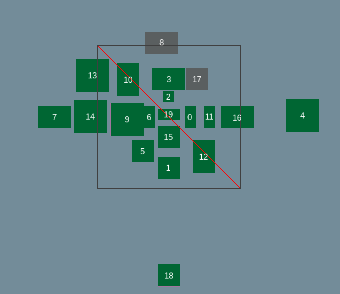
\includegraphics{./images/chap05-methodology/bad-solution-unmodified-gwo.png}
	\caption{Flowchart detailing the algorithm.}
	\label{bad-solution-unmodified-gwo}
\end{figure}

As one may infer, using the equations above will require setting an origin point for the buildings. Not considering the affinity of building towards the axes, having the origin point at the center or in a certain location in the bounding region restricts the possible locations where the buildings can cluster around. This restriction prevents us from exploring the solution subspace where solutions are feasible but where the cluster point is not the origin. This lead us to solutions that are less ideal. Aside from requiring setting the origin point, buildings moving towards the axes also presents another problem. Basing from our experiments, it prevents us from producing feasible solutions.

This behaviour can be attributed primarily to the formula, $\vec{D} = \left | \vec{C} \cdot \vec{X_{p}}(t) - \vec{X}(t) \right |$. To understand why the aforementioned formula contributes to the behaviour we have discussed earlier, we should understand what the formula means. It is helpful to simply consider that only building is being optimized in understanding the problems. Considering only the alpha solution may also provide better understanding as well.

Let us start with $\vec{C} \cdot \vec{X_{l}}(t)$ from $\vec{D} = \left | \vec{C} \cdot \vec{X_{l}}(t) - \vec{X}(t) \right |$. To simplify our explanation, let $K = \vec{C} \cdot \vec{X_{l}}(t)$. The range of each $i$th element in $K$ will be $[0, 2 \cdot \vec{C}_{l,i}]$. Note that the operation is a dot product, but it is actually pairwise multiplication. This means that $K$ simply scales the x and y positions, and angle of the buildings. Figure \ref{gwo-c-effect} shows a visualization of this effect. Despite the figure only showing the effect with a building's position in the first quadrant, the same effect can be observed with other buildings located in other quadrants. Now, considering the entirety of $\vec{D}$, $\vec{D}$ would mean to be the distance between a building $i$ moved to a different point in the region $S$ (see Figure \ref{gwo-c-effect}) in $\vec{X_{l}}$ and a building $i$ in $\vec{X}(t)$. A visualization for this is provided by Figure \ref{gwo-d-effect}.

\begin{figure}[h!]
	\centering
	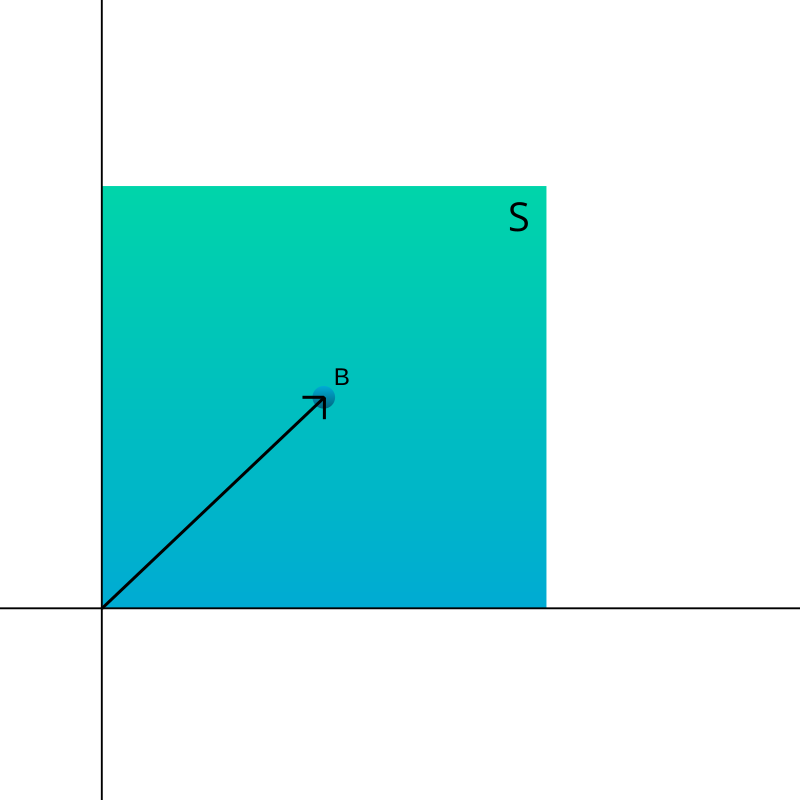
\includegraphics[scale=0.45]{./images/chap05-methodology/gwo-c-effect.png}
	\caption{In $K$, $C$ simply scales the x and y positions and angles of buildings. Assuming that the point $B$ represents the x and y positions of a building, the region $S$ is where $B$ may be repositioned based on the values of $C$.}
	\label{gwo-c-effect}
\end{figure}

\begin{figure}[h!]
	\centering
	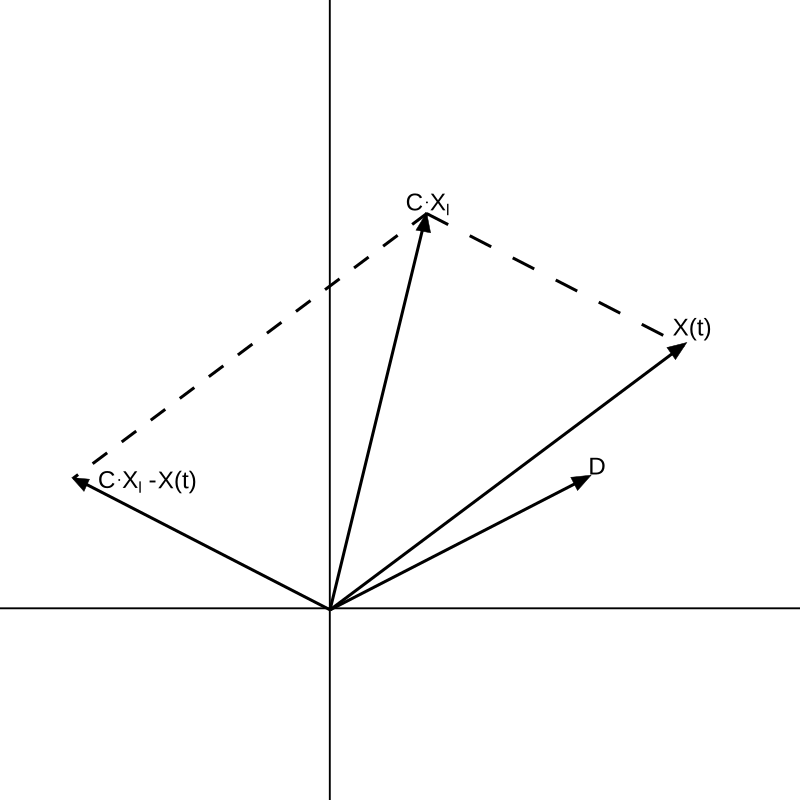
\includegraphics[scale=0.45]{./images/chap05-methodology/gwo-d-effect.png}
	\caption{A visualization of how $D$ is computed and its inherent meaning.}
	\label{gwo-d-effect}
\end{figure}

Let us also take note, $\vec{A} \cdot \vec{D}$. First, we should take note that $\vec{A} = 2 \cdot \vec{a} \cdot \vec{r_{1}} - \vec{a}$. $a$, as mentioned before, linearly decreases over time. Since $a$ decreases linearly over time, $\vec{A}$ will also decrease over time. This behaviour of $\vec{A}$ would mean that in $\vec{A} \cdot \vec{D}$, $\vec{D}$ will eventually decrease as well. Considering equations \ref{gwo-x1-eqn} to \ref{gwo-x3-eqn}, $\vec{A}$ influences the distance of a building from its counterpart in the leading wolves. This would mean that as the number of iterations increase in a run, buildings will eventually follow the placements of the leading wolves.

Let us now return back to $\vec{C} \cdot \vec{X_{l}}(t)$. Over the course of iterations, this equation will make it difficult for a building to change its position. Around 50\% of the time (due to the fact that $\vec{r_{2}}$ is a \textit{uniform} random vector), the value of $\vec{C}$ will be less than $1$. The position of the buildings will be moved towards the axes. Since $\vec{C}$ is a scaling factor, it will be difficult for a building position to move away from an axis. This affects all solutions, and noting that the leading wolves guide the entire population, the movement towards an axis will be propagated towards the entire population, especially with the fact that the $\vec{A}$ reduces the difference between the leading wolves/solutions and the rest of the solutions as the number of iterations increase in a run. Note that the penalty value for intersection prevents them from overlapping with one another. Buildings that are already on a certain axis will find it practically impossible to move in the direction of the perpendicular axis. Buildings that are on the origin itself will practically cease to move at all. Buildings will still be able to change their orientations, however. The reason for this behaviour of being stuck on an axis is due to the nature of axes themselves, where the value in one or both axes is zero, and to the scaling phenomenom caused by $\vec{C}$. Since $K = \vec{C} \cdot \vec{X_{l}}(t)$ and when a building is near or already on an axis, the x, y, or both x and y positions of a building will barely, if at all, move away from the axes it is currently stuck to, when multiplying with $\vec{C}$. Hence, the behaviour we are noticing.

The aforementioned formula makes the classical GWO inadequate for our problem instance. We are unable to produce feasible nor satisfying results. In order for the grey wolf optimization algorithm to be successfully adapted into solving the facility layout problems, we must introduce a few changes into the algorithm. These changes will be discussed in the next subsection.

\subsection{Modified GWO}
% Draft Note: We should maybe give a name to the modified GWO. Maybe call it "Ballais-Romero GWO variant". HAHAHA.

Mirjalili, S., Mirjalili, S., and Lewis, A. \cite{Mirjalili2014} included a figure similar to Figure \ref{gwo-positioning-update}. It visualizes how a wolf $\omega$ will update its position based on the information provided by the leading wolves.

\begin{figure}[h!]
	\centering
	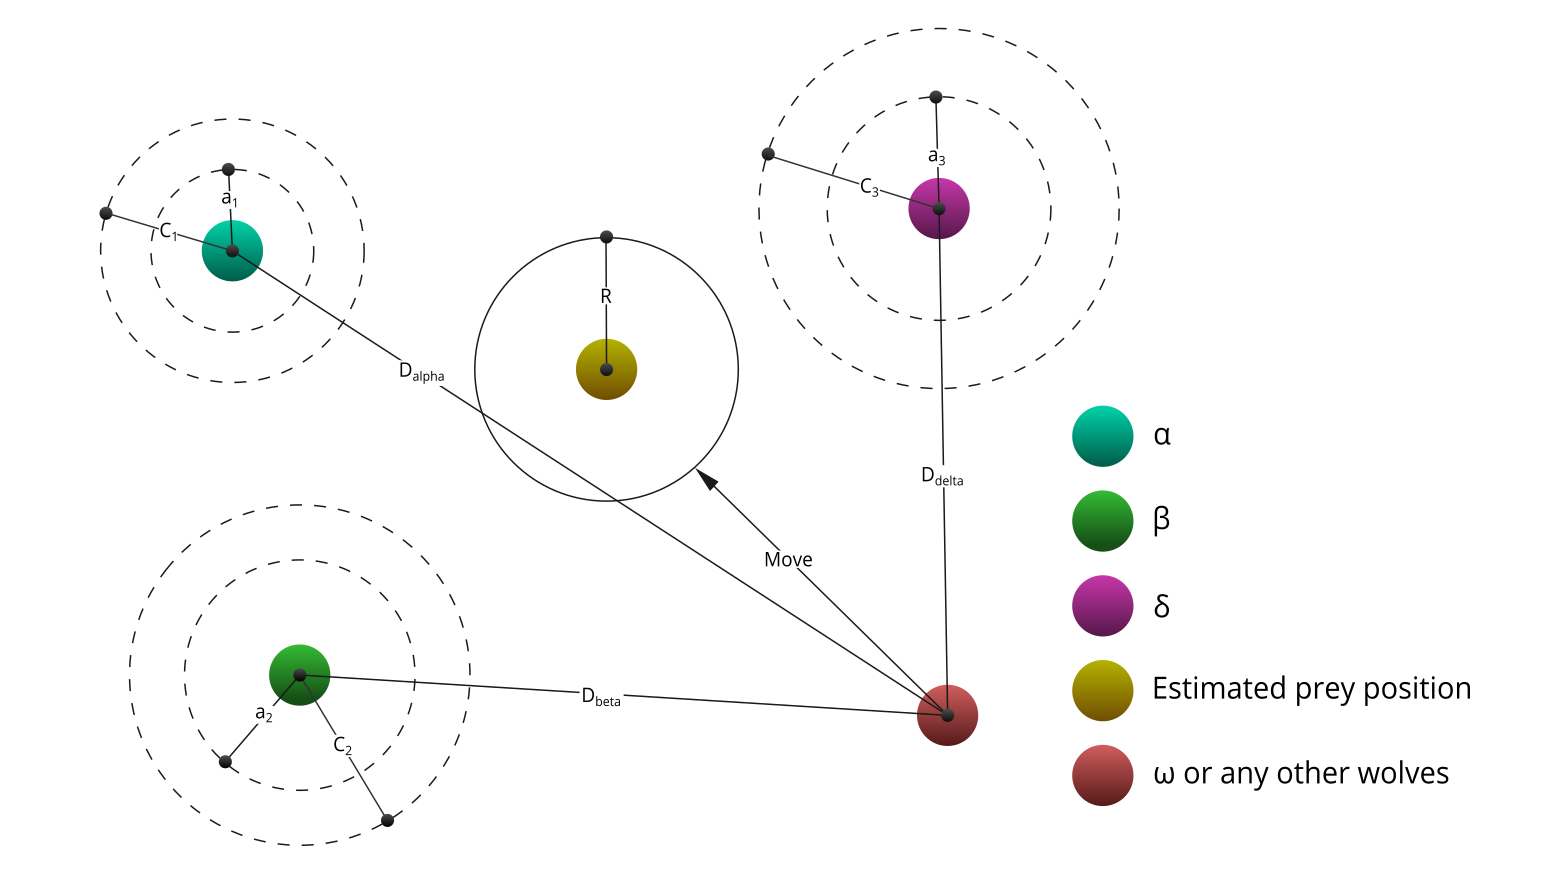
\includegraphics[scale=0.3]{./images/chap05-methodology/gwo-position-updating.png}
	\caption{Visualization of how wolves in GWO update their positions. An $\omega$ wolf will move towards a random point inside the circle of the estimated prey position.}
	\label{gwo-positioning-update}
\end{figure}

Basing from the visualization, notice that the $\vec{C}$ of the leading wolves specify the radius of the circle in which a $\vec{C} \cdot \vec{X_{l}}$ will be located it. The circle does \textbf{not} include an origin point. We have discussed before that performing a pairwise multiplication between $\vec{C}$ and $\vec{X_{l}}$ simply scales the elements $i$ in the vector $\vec{X_{l}}$. This is different from the visualization. To achieve the same effect as the visualization, instead of performing pairwise multiplication, we must utilize vector addition between $\vec{C}$ and $\vec{X_{l}}$. See Figure \ref{vector-addition-visualization} for a visualization of vector addition. This is the first modification we are introducing to classical GWO.

\begin{figure}[h!]
	\centering
	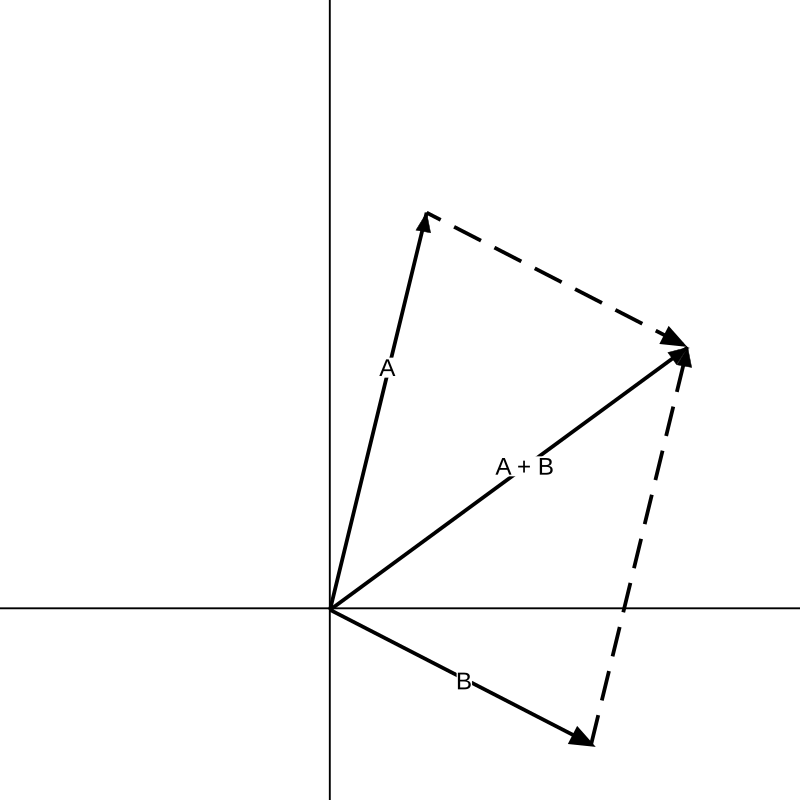
\includegraphics[scale=0.45]{./images/chap05-methodology/vector-addition-visualization.png}
	\caption{Vector addition pushes the point represented by $\vec{A}$ towards the direction of $\vec{B}$ by the magnitude of the same vector.}
	\label{vector-addition-visualization}
\end{figure}

In our modified GWO, $D$ is now defined as:

\begin{align}
	D &= \left | (\vec{C} + \vec{X_{l}}) - \vec{X}(t) \right | \label{modified-gwo-d}
\end{align}

However, this alone is not enough to comply with the aforementioned visualization. Using this will only move the buildings to the right and/or top. In order for us to move the buildings, we must also modify $\vec{C}$ as shown below:

\begin{align}
	C &= c \cdot \vec{r_{3}} \label{modified-gwo-c}
\end{align}

In this equation, $c$ is a real-valued variable, and $r_{3}$ is a random vector in $[-1, 1]$. This modification will now allow us to move a building from any direction and at any magnitude. The magnitude in which the building will be moved is controlled by $c$.

These modifications remove the necessity to specify an origin point in the bounding region, and the behaviour of buildings to move towards the origin or axes. Unfortunately, this alone is not enough to produce feasible results. We have to add two more modifications before we are able to produce good results.

The first additional modification is the building clamping. Each building is restricted to the boundary. If a building is moved towards outside the boundary, it will be pulled back to within the boundary. Building clamping can be mathematically defined as the following. Given a building $B$ in a solution $X(t)$ at iteration $t$ after being updated by Equations \ref{gwo-x1-eqn} to \ref{gwo-xt1-eqn}, \ref{modified-gwo-d}, and \ref{modified-gwo-c}, clamping can be mathematically modeled as:

\begin{align}
	B_{x} &= \text{max}\left (R_{x} + \frac{B_{w}}{2}, \text{min}\left(B_{x}, R_{x} + \left(R_{w} - \frac{B_{w}}{2}\right)\right)\right ) \label{bx-clamp-equation} \\
	B_{y} &= \text{max}\left (R_{y} + \frac{B_{h}}{2}, \text{min}\left(B_{y}, R_{y} + \left(R_{h} - \frac{B_{h}}{2}\right)\right)\right ) \label{by-clamp-equation}
\end{align}

where $B_{x}$ and $B_{y}$ are the $x$ and $y$ positions of the centroid of a building $B$, $B_{w}$ and $B_{h}$ are the width and height from the top left corner of a building $B$, $R_{x}$ and $R_{y}$ are the $x$ and $y$ positions of the top-left corner of the bounding region $R$, and $R_{w}$ and $R_{h}$ are the width and height of the bounding region $R$. Based on our prior experiments, without this clamping, buildings will freely move to points outside the boundary, and, at the end of the run, will produce a bad solution. 

This clamping should \textit{almost} solve the positioning of the buildings and allow us to produce results that are feasible. Since GWO is a continuous metaheuristic, building attributes that must only be one of two values will eventually be a value that is between the two aforementioned values. In our problem, this attribute that is affected is the building orientation. The building orientation may only be $0^{\circ}$ or $90^{\circ}$. It must never be a value between two. To solve this problem, we simply use the orientation of a building $B$ from the $\alpha$, $\beta$, or $\delta$ solutions, which are randomly selected. This idea is based off from the nature of GWO, where the best three solutions lead the search for the local optima. The building orientation of a building $B$ is, therefore, obtained using:

\begin{align}
	B_{o} = \left\{\begin{matrix}
		\alpha_{B_{o}} & \text{if } 0 \leq r < \frac{1}{3} \\ 
		\beta_{B_{o}}  & \text{if } \frac{1}{3} \leq r < \frac{2}{3}  \\ 
		\delta_{B_{o}} & \text{otherwise}
	\end{matrix}\right.
	\label{modified-gwo-bo}
\end{align}

where $B_{o}$ is the current orientation of a building $B$, $\alpha_{B_{o}}$, $\beta_{B_{o}}$, and $\delta_{B_{o}}$ are the orientations of building $B$ in the $\alpha$, $\beta$, and $\delta$ solutions, respectively, and $r$ is a random variable in $[0, 1]$. In our approach, assigning the building orientations is performed before clamping the buildings.

With all these modifications already discussed, we now need to briefly discuss how population initialization performed. The population is initialized by providing each building $B$ a random x and y position values, and random orientation. The orientation is either $0$ or $90$. The x and y positions are clamped as well to ensure that the buildings are inside the bounding region. The positions are clamped using Equations \ref{bx-clamp-equation} and \ref{by-clamp-equation}, respectively. Algorithm \ref{modified-gwo-algorithm-pop-initialization} shows the pseudocode for the population initialization.

\begin{algorithm}[h!]
\caption{Pseudocode for the population initialization.}
\label{modified-gwo-algorithm-pop-initialization}
\begin{algorithmic}[1]
\State Set $\vec{X}$ to be the solution.
\State Set $R_{x}$ to be the x position of the top-left corner of the bounding region $R$.
\State Set $R_{y}$ to be the y position of the top-left corner of bounding region $R$.
\State Set $R_{w}$ to be the width of the bounding region $R$.
\State Set $R_{h}$ to be the height of the bounding region $R$.
\State Set $N$ to be the number of buildings in a population.
\For{i = 0 until $N$}
	\State $\vec{X}_{(i * 3)}$ = $U(R_{x}, R_{x} + R_{w})$
	\State $\vec{X}_{(i * 3) + 1}$ = $U(R_{y}, R_{y} + R_{h})$
	\State $\vec{X}_{(i * 3) + 2}$ = $U({0, 90})$
	
	\State Apply Equation \ref{bx-clamp-equation} to $\vec{X}_{(i * 3)}$.
	\State Apply Equation \ref{by-clamp-equation} to $\vec{X}_{(i * 3) + 1}$.
\EndFor
\end{algorithmic}
\end{algorithm}

All these modifications for the classical GWO have allowed us to successfully adapt GWO to the facility layout problem. Equations \ref{summary-modified-gwo-a} to \ref{summary-modified-gwo-xt1}, and Algorithm \ref{modified-gwo-algorithm} summarises the entire modified GWO. Notice that these modifications are relatively simple, and do not significantly change the characteristics of classical GWO. The simplicity of GWO is still preserved. The next chapters will discuss how our modified version of GWO performs against configurations of unequal-area facility layout ptoblems.

\begin{align}
	\vec{A} &= 2\vec{a} \cdot \vec{r_{1}} - \vec{a} \label{summary-modified-gwo-a} \\
	\vec{C} &= c \cdot \vec{r_{2}} \\
	\vec{D}_{\alpha} &= \left | \left ( \vec{C}_{1} + \vec{X}_{\alpha} \right ) - \vec{X} \right | \label{summary-modified-gwo-DAlpha} \\
	\vec{D}_{\beta} &= \left | \left ( \vec{C}_{2} + \vec{X}_{\beta} \right ) - \vec{X} \right | \\
	\vec{D}_{\delta} &= \left | \left ( \vec{C}_{3} + \vec{X}_{\delta} \right ) - \vec{X} \right | \\
	\vec{X}_{1} &= \vec{X}_{\alpha} - \vec{A}_{1} \cdot \vec{D}_{\alpha} \\
	\vec{X}_{2} &= \vec{X}_{\beta} - \vec{A}_{2} \cdot \vec{D}_{\beta} \\
	\vec{X}_{3} &= \vec{X}_{\delta} - \vec{A}_{3} \cdot \vec{D}_{\delta} \\
	\vec{X}(t + 1) &= \frac{\vec{X}_{1} + \vec{X}_{2} + \vec{X}_{3}}{3} \label{summary-modified-gwo-xt1}
\end{align}

\begin{algorithm}[h!]
\caption{Pseudocode for the proposed modified GWO.}
\label{modified-gwo-algorithm}
\begin{algorithmic}[1]
\State Set $T$ to be the maximum number of iterations.
\State Initialize the grey wolf population $\vec{X}_{i} (i = 1, 2, \ldots, n)$
\State Initialize $c$, and $a = 2$.
\State Calculate the fitness of each wolf.
\State Set $\vec{X}_{\alpha}$ to be the fittest wolf.
\State Set $\vec{X}_{\beta}$ to be the second fittest wolf.
\State Set $\vec{X}_{\delta}$ to be the third fittest wolf.
\While{t $<$ T}
	\For{each wolf $\vec{X}_{i}$}
		\State Initialize $\vec{A}_{1}$, $\vec{A}_{2}$, $\vec{A}_{3}$, $\vec{C}_{1}$, $\vec{C}_{2}$, and $\vec{C}_{3}$.
		\State Update the position of the current wolf $\vec{X}_{i}$ using Equations \ref{summary-modified-gwo-DAlpha} to \ref{summary-modified-gwo-xt1}.
		\State Set the orientation of each building using Equation \ref{modified-gwo-bo}.
		\State Clamp the buildings in $\vec{X}_{i}$ using Equations \ref{bx-clamp-equation} and \ref{by-clamp-equation}.
	\EndFor
	\State Calculate the fitness of each wolf.
	\State Update $\vec{X}_{\alpha}$, $\vec{X}_{\beta}$, and $\vec{X}_{\delta}$.
	\State $a = 2 - \frac{2t}{T}$
	\State $t = t + 1$
\EndWhile \\
\Return $\vec{X}_{\alpha}$
\end{algorithmic}
\end{algorithm}

\section{Implementation Technologies}
Our program was developed using C++17 compiled using the Clang 11 compiler in an elementaryOS Hera environment under release mode with the \texttt{-03} optimized compilation flag turned on. Building was handled by CMake, and package management was handled by Conan. Our implementation is built on top of CoreX, a custom-developed 2D game engine. Using a game engine allowed us to visualize the results and configure experiments in a graphical manner. Using a custom engine over an over-the-shelf engine ensures that the implementation remains light and does not carry unnecessary features that are typically used in commercial game engines. The libraries EASTL, ImGUI, SDL 2, SDL 2 TTF. sdl-gpu, nlohmann JSON, and EnTT were used in developing the engine, with EnTT and ImGUI directly used by our implementation itself.
\chapter{Validation of the Approach}
Our proposed approach is validated by running it through a two data sets based off of the data sets used by Hasda, R., Bhattacharjya, R., and Bennis, F. (2017) \cite{Hasda2017} that will test its performance and compare it to a genetic algorithm-based approach. Basing from previous studies, the fitness of the solution produced by an approach determines the performance of an algorithm. As such, we will be comparing the average fitness values of our approach and the competiting approach. 30 feasible solutions are obtained with each approach and data set, and the fitnesses obtained in each run are averaged. Note that, however, only the fitnesses of feasible solutions are included in the average. Due to the non-deterministic nature of metaheuristics, infeasible solutions are bound to be generated.

\section{Data Sets Used}
Let us call the data sets used as problem configuration. Each problem configuration is based off of the configurations used by Hasda, R., Bhattacharjya, R., and Bennis, F. (2017) \cite{Hasda2017}. The first configuration used, which we will call SFLP-II, is shown in Table \ref{dataset-sflp-ii}, and the second configuration, which we will call mSFLP-III, is shown in Table ref{dataset-msflp-iii}. The second configuration is called as such due to the fact that it is a modification of the third problem configuration used by Hasda, R., Bhattacharjya, R., and Bennis, F.. SFLP-II uses a 12x12 bounding region, while mSFLP-III uses a 260x260 bounding region.

\begin{table}[h!]
\centering
\begin{tabular}{P{7mm}|P{7mm}|P{7mm}|P{7mm}|P{7mm}|P{7mm}|P{7mm}|P{7mm}|P{7mm}|P{7mm}|P{7mm}|}
	\cline{2-11}
	& \multicolumn{8}{c|}{Cost of Material Flow Between Buildings} & W & H \\ \cline{1-9}
	\multicolumn{1}{|l|}{Building} & 1     & 2     & 3     & 4     & 5     & 6     & 7     & 8    &       &        \\ \hline
	\multicolumn{1}{|l|}{1}        & 0     & 1     & 2     & 0     & 0     & 0     & 2     & 0    & 2     & 3      \\ \hline
	\multicolumn{1}{|l|}{2}        & 0     & 0     & 4     & 3     & 6     & 0     & 0     & 2    & 4     & 5      \\ \hline
	\multicolumn{1}{|l|}{3}        & 0     & 0     & 0     & 2     & 0     & 3     & 1     & 0    & 2     & 2      \\ \hline
	\multicolumn{1}{|l|}{4}        & 0     & 0     & 0     & 0     & 5     & 2     & 0     & 2    & 3     & 3      \\ \hline
	\multicolumn{1}{|l|}{5}        & 0     & 0     & 0     & 0     & 0     & 0     & 0     & 4    & 2     & 4      \\ \hline
	\multicolumn{1}{|l|}{6}        & 0     & 0     & 0     & 0     & 0     & 0     & 4     & 0    & 4     & 4      \\ \hline
	\multicolumn{1}{|l|}{7}        & 0     & 0     & 0     & 0     & 0     & 0     & 0     & 1    & 4     & 4      \\ \hline
	\multicolumn{1}{|l|}{8}        & 0     & 0     & 0     & 0     & 0     & 0     & 0     & 0    & 3     & 4      \\ \hline
\end{tabular}
\caption{Configuration of SFLP-II. W and H mean width and height, respectively.}
\label{dataset-sflp-ii}
\end{table}

\begin{table}
\begin{adjustwidth}{-0.85in}{}
\begin{tabular}{P{3mm}|P{3mm}|P{3mm}|P{3mm}|P{3mm}|P{3mm}|P{3mm}|P{3mm}|P{3mm}|P{3mm}|P{3mm}|P{3mm}|P{3mm}|P{3mm}|P{3mm}|P{3mm}|P{3mm}|P{3mm}|P{3mm}|P{3mm}|P{3mm}|P{3mm}|P{3mm}|}
	\cline{2-23}
	& \multicolumn{20}{c|}{Cost of Material Flow Between Buildings}                            & W & H \\ \cline{1-21}
	\multicolumn{1}{|l|}{Building} & 1 & 2 & 3 & 4 & 5 & 6 & 7 & 8 & 9 & 10 & 11 & 12 & 13 & 14 & 15 & 16 & 17 & 18 & 19 & 20 &       &        \\ \hline
	\multicolumn{1}{|l|}{1}        & 0 & 1 & 1 & 1 & 1 & 1 & 1 & 1 & 1 & 1  & 1  & 1  & 1  & 1  & 1  & 1  & 1  & 1  & 1  & 1  & 20    & 40     \\ \hline
	\multicolumn{1}{|l|}{2}        & 1 & 0 & 1 & 1 & 1 & 1 & 1 & 1 & 1 & 1  & 1  & 1  & 1  & 1  & 1  & 1  & 1  & 1  & 1  & 1  & 40    & 40     \\ \hline
	\multicolumn{1}{|l|}{3}        & 1 & 1 & 0 & 1 & 1 & 1 & 1 & 1 & 1 & 1  & 1  & 1  & 1  & 1  & 1  & 1  & 1  & 1  & 1  & 1  & 20    & 20     \\ \hline
	\multicolumn{1}{|l|}{4}        & 1 & 1 & 1 & 0 & 1 & 1 & 1 & 1 & 1 & 1  & 1  & 1  & 1  & 1  & 1  & 1  & 1  & 1  & 1  & 1  & 40    & 60     \\ \hline
	\multicolumn{1}{|l|}{5}        & 1 & 1 & 1 & 1 & 0 & 1 & 1 & 1 & 1 & 1  & 1  & 1  & 1  & 1  & 1  & 1  & 1  & 1  & 1  & 1  & 60    & 60     \\ \hline
	\multicolumn{1}{|l|}{6}        & 1 & 1 & 1 & 1 & 1 & 0 & 1 & 1 & 1 & 1  & 1  & 1  & 1  & 1  & 1  & 1  & 1  & 1  & 1  & 1  & 40    & 40     \\ \hline
	\multicolumn{1}{|l|}{7}        & 1 & 1 & 1 & 1 & 1 & 1 & 0 & 1 & 1 & 1  & 1  & 1  & 1  & 1  & 1  & 1  & 1  & 1  & 1  & 1  & 40    & 20     \\ \hline
	\multicolumn{1}{|l|}{8}        & 1 & 1 & 1 & 1 & 1 & 1 & 1 & 0 & 1 & 1  & 1  & 1  & 1  & 1  & 1  & 1  & 1  & 1  & 1  & 1  & 40    & 60     \\ \hline
	\multicolumn{1}{|l|}{9}        & 1 & 1 & 1 & 1 & 1 & 1 & 1 & 1 & 0 & 1  & 1  & 1  & 1  & 1  & 1  & 1  & 1  & 1  & 1  & 1  & 60    & 40     \\ \hline
	\multicolumn{1}{|l|}{10}       & 1 & 1 & 1 & 1 & 1 & 1 & 1 & 1 & 1 & 0  & 1  & 1  & 1  & 1  & 1  & 1  & 1  & 1  & 1  & 1  & 60    & 60     \\ \hline
	\multicolumn{1}{|l|}{11}       & 1 & 1 & 1 & 1 & 1 & 1 & 1 & 1 & 1 & 1  & 0  & 1  & 1  & 1  & 1  & 1  & 1  & 1  & 1  & 1  & 40    & 60     \\ \hline
	\multicolumn{1}{|l|}{12}       & 1 & 1 & 1 & 1 & 1 & 1 & 1 & 1 & 1 & 1  & 1  & 0  & 1  & 1  & 1  & 1  & 1  & 1  & 1  & 1  & 20    & 40     \\ \hline
	\multicolumn{1}{|l|}{13}       & 1 & 1 & 1 & 1 & 1 & 1 & 1 & 1 & 1 & 1  & 1  & 1  & 0  & 1  & 1  & 1  & 1  & 1  & 1  & 1  & 60    & 40     \\ \hline
	\multicolumn{1}{|l|}{14}       & 1 & 1 & 1 & 1 & 1 & 1 & 1 & 1 & 1 & 1  & 1  & 1  & 1  & 0  & 1  & 1  & 1  & 1  & 1  & 1  & 60    & 60     \\ \hline
	\multicolumn{1}{|l|}{15}       & 1 & 1 & 1 & 1 & 1 & 1 & 1 & 1 & 1 & 1  & 1  & 1  & 1  & 1  & 0  & 1  & 1  & 1  & 1  & 1  & 60    & 60     \\ \hline
	\multicolumn{1}{|l|}{16}       & 1 & 1 & 1 & 1 & 1 & 1 & 1 & 1 & 1 & 1  & 1  & 1  & 1  & 1  & 1  & 0  & 1  & 1  & 1  & 1  & 40    & 40     \\ \hline
	\multicolumn{1}{|l|}{17}       & 1 & 1 & 1 & 1 & 1 & 1 & 1 & 1 & 1 & 1  & 1  & 1  & 1  & 1  & 1  & 1  & 0  & 1  & 1  & 1  & 60    & 40     \\ \hline
	\multicolumn{1}{|l|}{18}       & 1 & 1 & 1 & 1 & 1 & 1 & 1 & 1 & 1 & 1  & 1  & 1  & 1  & 1  & 1  & 1  & 1  & 0  & 1  & 1  & 40    & 40     \\ \hline
	\multicolumn{1}{|l|}{19}       & 1 & 1 & 1 & 1 & 1 & 1 & 1 & 1 & 1 & 1  & 1  & 1  & 1  & 1  & 1  & 1  & 1  & 1  & 0  & 1  & 40    & 40     \\ \hline
	\multicolumn{1}{|l|}{20}       & 1 & 1 & 1 & 1 & 1 & 1 & 1 & 1 & 1 & 1  & 1  & 1  & 1  & 1  & 1  & 1  & 1  & 1  & 1  & 0  & 40    & 20     \\ \hline
\end{tabular}
\end{adjustwidth}
\caption{Configuration of mSFLP-III.}
\label{dataset-msflp-iii}
\end{table}

\section{Competiting Approach}
The competing GA approach, which we will compare our proposed GWO approach, contains multiple phases to solve the unequal area static facility layout problem. The basic framework of the algorithm is inspired from the works of Asl et al. (2015) \cite{Asl2015} and Asl, A. and Wong, K. (2015) \cite{Asl2015a}. We will be further discussing the algorithm in detail in this section.

\subsection{Population Generation}
In the competiting approach, the population generation is the same the method for initialization the population as the one in our proposed modified GWO approach.

\subsection{Swapping Method}
The swapping method is used to find a possible configuration for a solution that is better than the current configuration. This method is applied to all solutions in the population, but only in the first 100 iterations. Pseudocode for the swapping method is provided in Algorithm \ref{pseudocode-comp-ga-swapping}.

\begin{algorithm}
\caption{Pseudocode for the swapping method.}
\label{pseudocode-comp-ga-swapping}
\begin{algorithmic}[1]
\State Let $S$ be the collection of generated solutions.
\State Set $S_{curr}$ be the current solution.
\State Add $S_{curr}$ to $S$.
\State Set $N_{B}$ be the maximum number of buildings.
\For{i = 0 until $N_{B} - 2$}
	\For{j = i + 1 until $N_{B} - 1$}
		\State Building $i$'s orientation in $S_{curr}$ is changed to the other orientation,\WRP and the resulting new solution is added to $S$
		\State Building $j$'s orientation in $S_{curr}$ is changed to the other orientation,\WRP and the resulting new solution is added to $S$
		\State Building $i$'s and $j$'s orientations in $S_{curr}$ are changed to the other\WRP orientation, and the resulting new solution is added to $S$
		\State Building $i$'s and $j$'s positions are exchanged in $S_{curr}$, and the resulting new\WRP solutiA movement and a orientation changeon is added to $S$.
		\State Building $i$'s and $j$'s positions are exchanged in and the orientation of\WRP building $i$ is changed in $S_{curr}$, and the resulting new solution\WRP is added to $S$.
		\State Building $i$'s and $j$'s positions are exchanged in and the orientation of\WRP building $j$ is changed in $S_{curr}$, and the resulting new solution\WRP is added to $S$.
		\State Building $i$'s and $j$'s positions are exchanged in and the orientations of\WRP buildings $i$ and $j$ are changed in $S_{curr}$, and the resulting new solution\WRP is added to $S$.
	\EndFor
\EndFor \\
\Return the best solution in $S$.
\end{algorithmic}
\end{algorithm}

\subsection{Selection, Crossover, Mutation, and Elitism}
Key parts of a genetic algorithm are the selection, crossover, and mutation operators. These drive the algorithm to produce good solutions. We will be discussing each operator used in detail in this section. Elitism is also implemented in our proposed approach to ensure that the best solutions found so far do not get lost throughout iterations. It will also be discussed in this section.

\subsubsection{Selection}
The selection operator used in the competing approach is tournament selection. Tournament selection works by selecting $k$ (also known as tournament size) individuals from a population and using the best two selected individuals as parents for an offspring \cite{StackOverflow-TournamentSelection}. Algorithm \ref{pseudocode-tournament-selection} shows a pseudocode of tournament selection. Note that in the algorithm, $P_{p}$ denotes the $p$-th solution in $P$, and $|P|$ denotes the population size.

\begin{algorithm}
\caption{Pseudocode for the tournament selection.}
\label{pseudocode-tournament-selection}
\begin{algorithmic}[1]
\State Set $X^{(1)}$ to be the first best parent.
\State Set $X^{(2)}$ to be the second best parent.
\State Set $P$ to be the population of solutions.
\State Set $k$ to be the tournament size.
\State Set $f(X)$ to be the fitness function.
\State $X^{(1)} = \text{null}$
\State $X^{(2)} = \text{null}$
\For{$i = 1, 2,\ldots,k$}
	\State $p = U(1, |P|)$
	\If{$X^{(1)}== \text{null}$ or $f(P_{p}) < f(X^{(1)}$}
		\State $X_{(2)} = X^{(1)}$
		\State $X_{(1)} = P_{p}$
	\ElsIf{$X^{(2)}== \text{null}$ or $f(P_{p}) < f(X^{(2)}$}
		\State $X_{(2)} = P_{p}$
	\EndIf
\EndFor \\
\Return $X^{(1)}$, and $X^{(2)}$.
\end{algorithmic}
\end{algorithm}

\subsubsection{Crossover}
The crossover operator used in the competing approach is uniform crossover. Uniform crossover works by selecting a gene from a random parent and placing it in the offspring. This is applied for every gene in the offspring. Algorithm \ref{pseudocode-uniform-crossover} shows a pseudocode of uniform crossover.

\begin{algorithm}
\caption{Pseudocode for the uniform crossover.}
\label{pseudocode-uniform-crossover}
\begin{algorithmic}[1]
\State Set $X$ to be the offspring.
\State Set $N$ to be the number of genes a solution has.
\State Set $X^{(1)}$ to be the first parent.
\State Set $X^{(2)}$ to be the second parent.
\For{$i = 1, 2,\ldots, N$}
	\State $\text{rand} = U(0, 1)$
	\If{$\text{rand} < 0.5$}
		\State $X_{i} = X^{(1)}_{i}$
	\Else
		\State $X_{i} = X^{(2)}_{i}$
	\EndIf
\EndFor \\
\Return $X$.
\end{algorithmic}
\end{algorithm}

\subsubsection{Mutation}
Over time, as more and more iterations are performed, the diversity of the population will eventually be lost. To combat this, a mutation operator is performed to reintroduce diversity. The mutation operator used is an operator that we dub the "Buddy-Buddy Mutation".

The \textbf{Buddy-Buddy Mutation} is a mutation operator that simply selects two pairs of buildings $D$ and $S$, and move one of them to the side of the other building. Building $D$ is referred to as the dynamic buddy, while building $S$ is referred to as the static buddy. Building $D$ will be the building that will be moved towards the other building, which is building $S$ in our case. When moving building $D$, a side $E$ of building $S$ will first be randomly chosen. Afterwards, an orientation for building $D$ will be randomly chosen, whether it will be parallel or perpendicular to $E$. Once a side and orientation has been selected, building $D$ will be moved adjacent towards building $S$ at side $E$ with the chosen orientation. The implementation of this mutation operator in our proposed approach gives buildings that intersect with another building more chances of being selected as the dynamic buddy. Pseudocode and a visualization of the operator is provided by Algorithm \ref{pseudocode-buddybuddy-mutation} and Figure \ref{buddy-buddy-mutation-viz}, respectively.

\begin{algorithm}
\caption{Pseudocode for the Buddy-Buddy Mutation.}
\label{pseudocode-buddybuddy-mutation}
\begin{algorithmic}[1]
	\State Randomly select two buildings $D$ and $S$, with more weight given to buildings that are intersecting with another.
	\State Set $E$ to be a randomly selected side of building $S$.
	\State Set $O$ to either be a parallel or perpendicular orientation, randomly selected.
	\State Move building $D$ adjacent to side $E$ of building $S$ with the orientation $O$.
\end{algorithmic}
\end{algorithm}

\begin{figure}[h!]
	\centering
	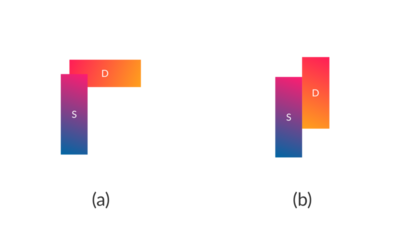
\includegraphics{./images/chap06-validation/buddy-buddy-mutation.png}
	\caption{Visualization of how Buddy-Buddy Mutation works. On the left are two buildings that are overlapping one another. The right shows the same buildings but with the mutation applied, causing them to no longer overlap. Note that the right shows only one possible arrangement for both buildings.}
	\label{buddy-buddy-mutation-viz}
\end{figure}

The rate at which a solution is mutated is highly dependent on the fitness of the solution. The worse the fitness of a solution is, the more likely it is to be mutated. This encourages the proposed algorithm to improve solutions that are generally bad. This rate scheme makes this an adaptive mutation operator \cite{Jiang2018}. The mutation rate is mathematically modelled as:

\begin{equation}
	m(X, t) = 1 - \frac{fit_{max}(t) - fit(X(t))}{fit_{max}(t) - fit_{min}(t)}
\end{equation}

where $m_{k}$ refers to the mutation rate of a solution $X$ at iteration $t$, $fit$ is a function that gets the fitness of a solution, and $fit_{min}$ and $fit_{max}$ gets the minimum and maximum fitnesses of the population, respectively.

\subsubsection{Elitism}
One variant of genetic algorithms includes elitism. This elitism allows a genetic algorithm to keep a number of best solutions in the next generation, ensuring that the best solutions do not get discarded over time. Note that this elitism strategy is not only limited to genetic algorithms. Other evolutionary algorithms may also utilize this strategy \cite{Du2018}. We are also taking this principle into our competing GA approach. In the competing approach, we are keeping the best $E_{N}$ solutions in the previous iteration to the next iteration.

\subsection{Local Searches}
Remember that our implementation is based on aforementioned previous works that used local search algorithms in conjunction to genetic algorithms. They combined GAs with local search algorithms because GAs find it hard to explore within the convergence area. Hybridizing it with a local search algorithm improves performance \cite{Ripon2013}. In our proposed approach, we are keeping this aspect of the previous works. This will also ensure that we are able to search within the convergence area more intensely and find better solutions. In the previous works and in ours, there are two local search algorithms, dubbed "Local Search 1" and "Local Search 2". They vary in terms of searching intensity, but both attempts to obtain better solutions. We will be discussing details of both in this section.

\subsubsection{Local Search 1}
The first local search algorithm, "Local Search 1", performs a local search by creating a number of solutions by moving each building in different directions by a certain random amount and changing its orientations after movement and obtaining the best solution from these activities. In our approach, the certain amount of movement is a random number between 1 and 5. This search algorithm is only applied to the best solution of the current iteration, and the best solution found in this search becomes the new best solution and replaces the previously best solution. The movements of each building is defined by a set of "activities". This set of activities is shown by Table \ref{local-search-1-activities}. Additionally, pseudocode of the search algorithm is shown in Algorithm \ref{pseudocode-local-search-1}.

\begin{table}[h!]
	\centering
	\begin{tabular}{| c | p{110mm} |}
		\hline
		Activity Number & Description \\
		\hline
		0 & A building is moved to the right along the x-axis by a random number between 1 and 5. \\
		1 & A building is moved to the left along the x-axis by a random number between 1 and 5. \\
		2 & A building is moved to the upwards along the y-axis by a random number between 1 and 5. \\
		3 & A building is moved to the downwards along the y-axis by a random number between 1 and 5. \\
		4 & Generate two random numbers from 1 and 5 and a building is moved to the right and then upward, respectively, by those numbers. \\
		5 & Generate two random numbers from 1 and 5 and a building is moved to the right and then downward, respectively, by those numbers. \\
		6 & Generate two random numbers from 1 and 5 and a building is moved to the left and then upward, respectively, by those numbers. \\
		7 & Generate two random numbers from 1 and 5 and a building is moved to the left and then downward, respectively, by those numbers. \\
		\hline
	\end{tabular}
	\caption{Activities for moving a building in Local Search 1}
	\label{local-search-1-activities}
\end{table}

\begin{algorithm}[h!]
\caption{Pseudocode for Local Search 1.}
\label{pseudocode-local-search-1}
\begin{algorithmic}[1]
\State Set $S$ to be a collection of solutions.
\State Set $S_{curr}$ to be the solution being optimized.
\State Add $S_{curr}$ to $S$.
\State Set $N_{B}$ be the maximum number of buildings.
\State Set $N_{A}$ be the maximum number of activities.
\For{i = 0 until $N_{B} - 1$}
	\For{a = 0 until $N_{B} - 1$}
		\State Perform activity $a$ with building $i$ in $S_{curr}$ and save the new solution in $S$.
		\State Perform activity $a$ with building $i$, and change the orientation of the building to the other orientation in $S_{curr}$ and save the new solution in $S$.
	\EndFor
\EndFor \\
\Return the best solution in $S$.
\end{algorithmic}
\end{algorithm}

\subsubsection{Local Search 2}
Local Search 2 is a more intense version of Local Search 1, in order to find the best solution so far. Unlike the latter that only moves one building at a time, Local Search 2 moves two buildings instead. The two buildings will also have their orientations changed after each activity. This local search is only applied to the best solution found in the last 50 iterations. The set of activities for this local search is shown by Table \ref{local-search-2-activities}, and a pseudocode of the search algorithm is shown in Algorithm \ref{pseudocode-local-search-2}.

\begin{algorithm}[h!]
	\caption{Pseudocode for Local Search 2.}
	\label{pseudocode-local-search-2}
	\begin{algorithmic}[1]
		\State Set $S$ to be a collection of solutions.
		\State Set $S_{curr}$ to be the solution being optimized.
		\State Add $S_{curr}$ to $S$.
		\State Set $N_{B}$ be the maximum number of buildings.
		\State Set $N_{A}$ be the maximum number of activities.
		\For{i = 0 until $N_{B} - 2$}
		\For{a = 0 until $N_{B} - 1$}
		\State Perform activity $a$ with building $i$ in $S_{curr}$ and save the new solution in $S$.
		\State Perform activity $a$ with building $i$, and change the orientation of \WRP building $i$ to the other orientation in $S_{curr}$ and save the new \WRP solution in $S$.
		\State Perform activity $a$ with building $i$, and change the orientation of \WRP building $i + 1$ to the other orientation in $S_{curr}$ and save the new \WRP solution in $S$.
		\State Perform activity $a$ with building $i$, and change the orientations of \WRP buildings $i$ and $i + 1$ to the other orientations in $S_{curr}$ and save the new \WRP solution in $S$.
		\EndFor
		\EndFor \\
		\Return the best solution in $S$.
	\end{algorithmic}
\end{algorithm}

\begin{longtable}{| c | p{120mm} |}
	\hline
	Activity Number & Description \\
	\hline
	0  & Building $i$ and $i + 1$ are moved to the right along the x-axis by a random number between 1 and 5. \\
	1  & Building $i$ and $i + 1$ are moved to the left along the x-axis by a random number between 1 and 5. \\
	2  & Building $i$ and $i + 1$ are moved upwards along the x-axis by a random number between 1 and 5. \\
	3  & Building $i$ and $i + 1$ are moved downwards along the x-axis by a random number between 1 and 5. \\
	4  & Generate two random numbers from 1 and 5 and buildings $i$ and $i + 1$ are moved to the right and then upward, respectively, by those numbers. \\
	5  & Generate two random numbers from 1 and 5 and buildings $i$ and $i + 1$ are moved to the right and then downward, respectively, by those numbers. \\
	6  & Generate two random numbers from 1 and 5 and buildings $i$ and $i + 1$ are moved to the left and then upward, respectively, by those numbers. \\
	7  & Generate two random numbers from 1 and 5 and buildings $i$ and $i + 1$ are moved to the left and then downward, respectively, by those numbers. \\
	8  & Generate two random numbers $a$ and $b$ that are from 1 to 5, and building $i$ is moved upward by $a$ and building $i + 1$ is moved to the right by $b$. \\
	9  & Generate two random numbers $a$ and $b$ that are from 1 to 5, and building $i$ is moved upward by $a$ and building $i + 1$ is moved downward by $b$. \\
	10 & Generate two random numbers $a$ and $b$ that are from 1 to 5, and building $i$ is moved upward by $a$ and building $i + 1$ is moved to the left by $b$. \\
	11 & Generate two random numbers $a$ and $b$ that are from 1 to 5, and building $i$ is moved to the right by $a$ and building $i + 1$ is moved downward by $b$. \\
	12 & Generate two random numbers $a$ and $b$ that are from 1 to 5, and building $i$ is moved to the right by $a$ and building $i + 1$ is moved upward by $b$. \\
	13 & Generate two random numbers $a$ and $b$ that are from 1 to 5, and building $i$ is moved to the right by $a$ and building $i + 1$ is moved to the left by $b$. \\
	14 & Generate two random numbers $a$ and $b$ that are from 1 to 5, and building $i$ is moved to the left by $a$ and building $i + 1$ is moved to downward by $b$. \\
	15 & Generate two random numbers $a$ and $b$ that are from 1 to 5, and building $i$ is moved to the left by $a$ and building $i + 1$ is moved to the right by $b$. \\
	16 & Generate two random numbers $a$ and $b$ that are from 1 to 5, and building $i$ is moved to the left by $a$ and building $i + 1$ is moved upward by $b$. \\
	17 & Generate two random numbers $a$ and $b$ that are from 1 to 5, and building $i$ is moved downward by $a$ and building $i + 1$ is moved to the right by $b$. \\
	18 & Generate two random numbers $a$ and $b$ that are from 1 to 5, and building $i$ is moved downward by $a$ and building $i + 1$ is moved to the left by $b$. \\
	19 & Generate two random numbers $a$ and $b$ that are from 1 to 5, and building $i$ is moved downward by $a$ and building $i + 1$ is moved upward by $b$. \\
	\hline
	\caption{Activities for moving a building in Local Search 2}
	\label{local-search-2-activities}
\end{longtable}

\subsubsection{Competing Algorithm Summarized}
The entire competing GA algorithm is summarized in pseudocode with Algorithm \ref{pseudocode-ga-approach}. Note that our implementation of the competing GA algorithm produces two children during the crossover phase. If there is no space for the second child in the current geenration, the worst offspring will be replaced by the second child.

\begin{algorithm}
\caption{Pseudocode for the competing GA approach.}
\label{pseudocode-ga-approach}
\begin{algorithmic}[1]
\State Initialize population $P$.
\State Calculate the fitness of each solution in $P$.
\State Set $T$ to be the number of generations.
\State Set $X^{(best)}$ to be the best solution found.
\State Set $E_{N}$ to be the number of elite solutions that will be kept in the next generation.
\State Sort $P$ from lowest to highest fitness value.
\For{$t = 1, 2, \ldots T$}
	\If{$t \leq 100$}
		\State Apply swapping method.
	\EndIf
	\For{$i = E_{N} + 1, \ldots, |P|$}
		\State Select parents $X^{(1)}$ and $X^{(2)}$ using tournament selection.
		\State Crossover parents and produce offspring $X^{(o)}$.
		\State Mutate $X^{(o)}$ if mutation probability allows.
		\State $P_{i} = X^{(o)}$.
	\EndFor
	\State Sort $P$ from lowest to highest fitness value.
	\State Apply Local Search 1 to the best solution in $P$.
	\If{$t \geq T - 50$}
		\State Apply Local Search 2 to the best solution in $P$.
	\EndIf
\EndFor \\
\Return best solution in $P$.
\end{algorithmic}
\end{algorithm}
\chapter{Results and Discussion}
The results of our experiments with our data set will be presented in this chapter. 30 runs of each approach that produced feasible solutions are included in the results. Note that some runs produce an infeasible solution. This due to the non-deterministic nature of metaheuristics, which will cause it to produce infeasible solutions sometimes.

\section{Environment}
All of the approaches were run in the following hardware and software configurations:

\begin{itemize}
	\item Hardware
	\begin{itemize}
		\item \textbf{CPU}: AMD Ryzen 5 5600X
		\item \textbf{GPU}: NVIDIA GeForce GTX 1050 Ti
		\item \textbf{RAM}: Crucial Ballistix RGB 3600 MHz DDR4 16 GB (8 GB x 2) CL16
	\end{itemize}
	\item Software
	\begin{itemize}
		\item \textbf{OS}: elementaryOS 5.1.7 Hera
		\item \textbf{Linux Kernel Version}: 5.4.0-99-generic
	\end{itemize}
\end{itemize}

\section{Experiments}
We have conducted two sets of experiments in order for us to evaluate the performance of our proposed GWO approach. The first set of experiments varies the GWO parameter, $c$, and the population size. It shows the impact of the parameters to the algorithm. The second set are experiments with the competing approaches. It shows how our proposed approach compares against other approaches. A population size of $50$ is used for all the experiment runs in the second set. This set will then be compared to the GWO experiment runs that have a population of the same size.

\subsection{Results with Different GWO Parameter Values}
Our proposed GWO approach only has one parameter, other than the population size, and number of iterations, the $c$ value. We used four values for the parameter: $2$, $4$, $8$, and $12$. We also varied the population size for this experiment set. The population sizes we used are: $25$, $50$, and $75$. Tables \ref{approach-gwo-c2-p25-results} to \ref{approach-gwo-c12-p75-results} show the results. We will refer to each GWO experiment as $G_{n,c}$, where $n$ is the population size, and $c$ is the value of the $c$ parameter in each experiment. So, for example, the GWO experiment with a population size of $25$ and $c = 2$ will be referred to as $G_{25,2}$, and so on. Each experiment for each parameter configuration combination has been run 30 times.

% Start of the GWO table of results for the one with a population of 25.
\begin{table}[h!]
\begin{adjustwidth}{-1.18in}{}
	\centering
	\begin{tabular}{|l|l|l|l|l|l|}
	\hline
	\multicolumn{1}{|c|}{\multirow{2}{*}{\textbf{Problem}}} & \multicolumn{5}{c|}{\textbf{GWO (c = 2, Pop. Size of 25)}} \\ \cline{2-6} 
	\multicolumn{1}{|c|}{}                                  & \multicolumn{1}{c|}{\textbf{Best}} & \multicolumn{1}{c|}{\textbf{Worst}} & \multicolumn{1}{c|}{\textbf{Avg.}} & \multicolumn{1}{c|}{\textbf{Std. Dev.}} & \multicolumn{1}{c|}{\textbf{Avg. Runtime (s)}} \\ \hline
	SFLP-II                                                 & 226.149871                                  & 328.546146                                   & 287.749326366667                      & 24.7018482581174                                 & 6.03333333333333                                  \\ \hline
	mSFLP-III                                               & 50874.238564                                & 60974.998642                                 & 55624.0061857667						         & 2544.70550235336                              & 22.4333333333333                               \\ \hline
	mKra30a                                               & 94640.759514                                & 120397.403767                                 &
	107874.742523333							&
	6706.6049593287							&
	35.9666666666667						\\ \hline
	\end{tabular}
\end{adjustwidth}
\caption{Results obtained from our proposed GWO approach with $c = 2$ and a population of $25$.}
\label{approach-gwo-c2-p25-results}
\end{table}

\begin{table}[h!]
\begin{adjustwidth}{-1.18in}{}
	\centering
	\begin{tabular}{|l|l|l|l|l|l|}
	\hline
	\multicolumn{1}{|c|}{\multirow{2}{*}{\textbf{Problem}}} & \multicolumn{5}{c|}{\textbf{GWO (c = 4, Pop. Size of 25)}} \\ \cline{2-6} 
	\multicolumn{1}{|c|}{}                                  & \multicolumn{1}{c|}{\textbf{Best}} & \multicolumn{1}{c|}{\textbf{Worst}} & \multicolumn{1}{c|}{\textbf{Avg.}} & \multicolumn{1}{c|}{\textbf{Std. Dev.}} & \multicolumn{1}{c|}{\textbf{Avg. Runtime (s)}} \\ \hline
	SFLP-II                                                 & 228.710226                                  & 373.604858                                   & 298.836421533333                      & 34.1522620177737                                 & 5.9                                  \\ \hline
	mSFLP-III                                               & 50825.278824                                & 59194.486832                                 & 55236.4286594						         & 2301.71070299619                              & 21.3333333333333                               \\ \hline
	mKra30a                                               & 87110.57618                                & 116746.599121                                 &
	104270.487286567							&
	8041.05756072353							&
	36.3333333333333						\\ \hline
	\end{tabular}
\end{adjustwidth}
\caption{Results obtained from our proposed GWO approach with $c = 4$ and a population of $25$.}
\label{approach-gwo-c4-p25-results}
\end{table}

\begin{table}[h!]
\begin{adjustwidth}{-1.18in}{}
	\centering
	\begin{tabular}{|l|l|l|l|l|l|}
	\hline
	\multicolumn{1}{|c|}{\multirow{2}{*}{\textbf{Problem}}} & \multicolumn{5}{c|}{\textbf{GWO (c = 8, Pop. Size of 25)}} \\ \cline{2-6} 
	\multicolumn{1}{|c|}{}                                  & \multicolumn{1}{c|}{\textbf{Best}} & \multicolumn{1}{c|}{\textbf{Worst}} & \multicolumn{1}{c|}{\textbf{Avg.}} & \multicolumn{1}{c|}{\textbf{Std. Dev.}} & \multicolumn{1}{c|}{\textbf{Avg. Runtime (s)}} \\ \hline
	SFLP-II                                                 & 249.624192                                  & 368.435807                                   & 313.640670633333                     & 29.7958232730557                                 & 6.23333333333333                                  \\ \hline
	mSFLP-III                                               & 51250.638187                                & 57894.186882                                 & 54206.6467008333						         & 1334.40810225102                              & 23.6                               \\ \hline
	mKra30a                                               & 95254.061554                                & 118719.490257                                 &
	105760.743434367							&
	6557.69877516131							&
	37.0666666666667						\\ \hline
	\end{tabular}
\end{adjustwidth}
\caption{Results obtained from our proposed GWO approach with $c = 8$ and a population of $25$.}
\label{approach-gwo-c8-p25-results}
\end{table}

\begin{table}[h!]
\begin{adjustwidth}{-1.18in}{}
	\centering
	\begin{tabular}{|l|l|l|l|l|l|}
	\hline
	\multicolumn{1}{|c|}{\multirow{2}{*}{\textbf{Problem}}} & \multicolumn{5}{c|}{\textbf{GWO (c = 12, Pop. Size of 25)}} \\ \cline{2-6} 
	\multicolumn{1}{|c|}{}                                  & \multicolumn{1}{c|}{\textbf{Best}} & \multicolumn{1}{c|}{\textbf{Worst}} & \multicolumn{1}{c|}{\textbf{Avg.}} & \multicolumn{1}{c|}{\textbf{Std. Dev.}} & \multicolumn{1}{c|}{\textbf{Avg. Runtime (s)}} \\ \hline
	SFLP-II                                                 & 255.639347                                  & 358.033844                                   & 315.207093933333                      & 26.4399229476443                                 & 6.36666666666667                                  \\ \hline
	mSFLP-III                                               & 51328.437737                                & 62758.004044                                 & 55331.2312675333						         & 2540.54370041386                              & 21.2333333333333                              \\ \hline
	mKra30a                                               & 93525.765816                                & 124181.531029                                 &
	108251.9895637							&
	8151.19724950765							&
	37.3						\\ \hline
	\end{tabular}
\end{adjustwidth}
\caption{Results obtained from our proposed GWO approach with $c = 12$ and a population of $25$.}
\label{approach-gwo-c12-p25-results}
\end{table}

% Start of the GWO table of results for the one with a population of 50.
\begin{table}[h!]
	\begin{adjustwidth}{-1.18in}{}
		\centering
		\begin{tabular}{|l|l|l|l|l|l|}
			\hline
			\multicolumn{1}{|c|}{\multirow{2}{*}{\textbf{Problem}}} & \multicolumn{5}{c|}{\textbf{GWO (c = 2, Pop. Size of 50)}} \\ \cline{2-6} 
			\multicolumn{1}{|c|}{}                                  & \multicolumn{1}{c|}{\textbf{Best}} & \multicolumn{1}{c|}{\textbf{Worst}} & \multicolumn{1}{c|}{\textbf{Avg.}} & \multicolumn{1}{c|}{\textbf{Std. Dev.}} & \multicolumn{1}{c|}{\textbf{Avg. Runtime (s)}} \\ \hline
			SFLP-II                                                 & 221.18019                                  & 341.568304                                   & 283.795019233333                      & 28.9742518867792                                 & 13.2666666666667                                  \\ \hline
			mSFLP-III                                               & 47597.794662                                & 62827.738159                                 & 54495.2676476667						         & 3328.18744058766                              & 40.1333333333333                               \\ \hline
			mKra30a                                               & 88657.824898                                & 121124.59779                                 &
			102742.1803823							&
			7156.18271087496							&
			73.3333333333333						\\ \hline
		\end{tabular}
	\end{adjustwidth}
	\caption{Results obtained from our proposed GWO approach with $c = 2$ and a population of $50$.}
	\label{approach-gwo-c2-p50-results}
\end{table}

\begin{table}[h!]
	\begin{adjustwidth}{-1.18in}{}
		\centering
		\begin{tabular}{|l|l|l|l|l|l|}
			\hline
			\multicolumn{1}{|c|}{\multirow{2}{*}{\textbf{Problem}}} & \multicolumn{5}{c|}{\textbf{GWO (c = 4, Pop. Size of 50)}} \\ \cline{2-6} 
			\multicolumn{1}{|c|}{}                                  & \multicolumn{1}{c|}{\textbf{Best}} & \multicolumn{1}{c|}{\textbf{Worst}} & \multicolumn{1}{c|}{\textbf{Avg.}} & \multicolumn{1}{c|}{\textbf{Std. Dev.}} & \multicolumn{1}{c|}{\textbf{Avg. Runtime (s)}} \\ \hline
			SFLP-II                                                 & 241.862298                                  & 389.711568                                   & 294.2461242                      & 33.7641257773172                                 & 13.1333333333333                                  \\ \hline
			mSFLP-III                                               & 50250.080536                                & 57916.673454                                 & 53421.9267731333						         & 2239.06725435468                              & 41.9666666666667                               \\ \hline
			mKra30a                                               & 90599.06601                                & 122300.269909                                 &
			102855.4831497							&
			8820.10238434929							&
			70.9666666666667						\\ \hline
		\end{tabular}
	\end{adjustwidth}
	\caption{Results obtained from our proposed GWO approach with $c = 4$ and a population of $50$.}
	\label{approach-gwo-c4-p50-results}
\end{table}

\begin{table}[h!]
	\begin{adjustwidth}{-1.18in}{}
		\centering
		\begin{tabular}{|l|l|l|l|l|l|}
			\hline
			\multicolumn{1}{|c|}{\multirow{2}{*}{\textbf{Problem}}} & \multicolumn{5}{c|}{\textbf{GWO (c = 8, Pop. Size of 50)}} \\ \cline{2-6} 
			\multicolumn{1}{|c|}{}                                  & \multicolumn{1}{c|}{\textbf{Best}} & \multicolumn{1}{c|}{\textbf{Worst}} & \multicolumn{1}{c|}{\textbf{Avg.}} & \multicolumn{1}{c|}{\textbf{Std. Dev.}} & \multicolumn{1}{c|}{\textbf{Avg. Runtime (s)}} \\ \hline
			SFLP-II                                                 & 240.638127                                  & 413.077936                                   & 299.553292466667                     & 40.469222577263                                 & 12.7333333333333                                  \\ \hline
			mSFLP-III                                               & 48844.175789                                & 59710.615997                                 & 52699.5983075667						         & 2062.76885562279                              & 41.2666666666667                               \\ \hline
			mKra30a                                               & 84929.672058                                & 112251.415863                                 &
			101570.163644533							&
			6490.61277032704							&
			72.1						\\ \hline
		\end{tabular}
	\end{adjustwidth}
	\caption{Results obtained from our proposed GWO approach with $c = 8$ and a population of $50$.}
	\label{approach-gwo-c8-p50-results}
\end{table}

\begin{table}[h!]
	\begin{adjustwidth}{-1.18in}{}
		\centering
		\begin{tabular}{|l|l|l|l|l|l|}
			\hline
			\multicolumn{1}{|c|}{\multirow{2}{*}{\textbf{Problem}}} & \multicolumn{5}{c|}{\textbf{GWO (c = 12, Pop. Size of 50)}} \\ \cline{2-6} 
			\multicolumn{1}{|c|}{}                                  & \multicolumn{1}{c|}{\textbf{Best}} & \multicolumn{1}{c|}{\textbf{Worst}} & \multicolumn{1}{c|}{\textbf{Avg.}} & \multicolumn{1}{c|}{\textbf{Std. Dev.}} & \multicolumn{1}{c|}{\textbf{Avg. Runtime (s)}} \\ \hline
			SFLP-II                                                 & 261.869799                                  & 381.586061                                   & 315.831642166667                      & 31.7204847308938                                 & 13.6666666666667                                  \\ \hline
			mSFLP-III                                               & 48920.979538                                & 56477.689476                                 & 52837.3591700333						         & 1980.22102755171                              & 42.2333333333333                              \\ \hline
			mKra30a                                               & 92563.720146                                & 128598.716599                                 &
			105348.4949903							&
			9267.72959691125							&
			69.5666666666667						\\ \hline
		\end{tabular}
	\end{adjustwidth}
	\caption{Results obtained from our proposed GWO approach with $c = 12$ and a population of $50$.}
	\label{approach-gwo-c12-p50-results}
\end{table}

% Start of the GWO table of results for the one with a population of 75.
\begin{table}[h!]
	\begin{adjustwidth}{-1.18in}{}
		\centering
		\begin{tabular}{|l|l|l|l|l|l|}
			\hline
			\multicolumn{1}{|c|}{\multirow{2}{*}{\textbf{Problem}}} & \multicolumn{5}{c|}{\textbf{GWO (c = 2, Pop. Size of 75)}} \\ \cline{2-6} 
			\multicolumn{1}{|c|}{}                                  & \multicolumn{1}{c|}{\textbf{Best}} & \multicolumn{1}{c|}{\textbf{Worst}} & \multicolumn{1}{c|}{\textbf{Avg.}} & \multicolumn{1}{c|}{\textbf{Std. Dev.}} & \multicolumn{1}{c|}{\textbf{Avg. Runtime (s)}} \\ \hline
			SFLP-II                                                 & 205.666955                                  & 386.356476                                   & 290.063388433333                      & 38.0436802516604                                 & 18.8666666666667                                  \\ \hline
			mSFLP-III                                               & 50179.684898                                & 57659.66436                                 & 54015.3749653						         & 2050.7167136713                              & 61.1                               \\ \hline
			mKra30a                                               & 88740.484344                                & 117173.305939                                 &
			99149.0616948							&
			5833.24082935413							&
			104.7						\\ \hline
		\end{tabular}
	\end{adjustwidth}
	\caption{Results obtained from our proposed GWO approach with $c = 2$ and a population of $75$.}
	\label{approach-gwo-c2-p75-results}
\end{table}

\begin{table}[h!]
	\begin{adjustwidth}{-1.18in}{}
		\centering
		\begin{tabular}{|l|l|l|l|l|l|}
			\hline
			\multicolumn{1}{|c|}{\multirow{2}{*}{\textbf{Problem}}} & \multicolumn{5}{c|}{\textbf{GWO (c = 4, Pop. Size of 75)}} \\ \cline{2-6} 
			\multicolumn{1}{|c|}{}                                  & \multicolumn{1}{c|}{\textbf{Best}} & \multicolumn{1}{c|}{\textbf{Worst}} & \multicolumn{1}{c|}{\textbf{Avg.}} & \multicolumn{1}{c|}{\textbf{Std. Dev.}} & \multicolumn{1}{c|}{\textbf{Avg. Runtime (s)}} \\ \hline
			SFLP-II                                                 & 239.258536                                  & 406.790997                                   & 302.005947566667                      & 39.1344289013742                                 & 18.9                                  \\ \hline
			mSFLP-III                                               & 48752.443314                                & 56156.624268                                 & 52037.6629276						         & 2313.4004317195                              & 61.5333333333333                               \\ \hline
			mKra30a                                               & 89197.608078                                & 121878.61042                                 &
			99482.2352776							&
			7069.6968084522							&
			107.966666666667						\\ \hline
		\end{tabular}
	\end{adjustwidth}
	\caption{Results obtained from our proposed GWO approach with $c = 4$ and a population of $75$.}
	\label{approach-gwo-c4-p75-results}
\end{table}

\begin{table}[h!]
	\begin{adjustwidth}{-1.18in}{}
		\centering
		\begin{tabular}{|l|l|l|l|l|l|}
			\hline
			\multicolumn{1}{|c|}{\multirow{2}{*}{\textbf{Problem}}} & \multicolumn{5}{c|}{\textbf{GWO (c = 8, Pop. Size of 75)}} \\ \cline{2-6} 
			\multicolumn{1}{|c|}{}                                  & \multicolumn{1}{c|}{\textbf{Best}} & \multicolumn{1}{c|}{\textbf{Worst}} & \multicolumn{1}{c|}{\textbf{Avg.}} & \multicolumn{1}{c|}{\textbf{Std. Dev.}} & \multicolumn{1}{c|}{\textbf{Avg. Runtime (s)}} \\ \hline
			SFLP-II                                                 & 246.916627                                  & 393.744452                                   & 309.957982766667                     & 32.0156308267039                                 & 19.5                                  \\ \hline
			mSFLP-III                                               & 49276.248596                                & 54977.558044                                 & 51801.8837937333						         & 1419.1918023338                              & 63.0333333333333                               \\ \hline
			mKra30a                                               & 87299.715054                                & 113760.078079                                 &
			98968.6223121							&
			6443.60722715266							&
			108.7						\\ \hline
		\end{tabular}
	\end{adjustwidth}
	\caption{Results obtained from our proposed GWO approach with $c = 8$ and a population of $75$.}
	\label{approach-gwo-c8-p75-results}
\end{table}

\begin{table}[h!]
	\begin{adjustwidth}{-1.18in}{}
		\centering
		\begin{tabular}{|l|l|l|l|l|l|}
			\hline
			\multicolumn{1}{|c|}{\multirow{2}{*}{\textbf{Problem}}} & \multicolumn{5}{c|}{\textbf{GWO (c = 12, Pop. Size of 75)}} \\ \cline{2-6} 
			\multicolumn{1}{|c|}{}                                  & \multicolumn{1}{c|}{\textbf{Best}} & \multicolumn{1}{c|}{\textbf{Worst}} & \multicolumn{1}{c|}{\textbf{Avg.}} & \multicolumn{1}{c|}{\textbf{Std. Dev.}} & \multicolumn{1}{c|}{\textbf{Avg. Runtime (s)}} \\ \hline
			SFLP-II                                                 & 243.386427                                  & 413.874466                                   & 307.3213231                      & 36.2239957721235                                 & 19.3333333333333                                  \\ \hline
			mSFLP-III                                               & 49644.232903                                & 55524.684891                                 & 51837.8766529667						         & 1430.57988385005                              & 61.7666666666667                              \\ \hline
			mKra30a                                               & 86942.304199                                & 108422.175175                                 &
			98108.9092933667							&
			6511.43059062118							&
			111.266666666667						\\ \hline
		\end{tabular}
	\end{adjustwidth}
	\caption{Results obtained from our proposed GWO approach with $c = 12$ and a population of $75$.}
	\label{approach-gwo-c12-p75-results}
\end{table}

Let us first discuss the results with the SFLP-II problem. Table \ref{full-data-gwo-sflp-ii} provides a summary of the results of the experiments performed for the problem using the GWO approach. For the problem, $G_{50,2}$ has the best average compared to the other configurations with a value of $283.795019233333$. The worst average belonged to $G_{50,12}$ with a value of $315.831642166667$. The configuration with the best solution produced would be $G_{75,2}$ with the solution having a value of $205.666955$. On the other hand, the worst solution was produced by $G_{75,12}$ with a value of $413.874466$. The average runtime of the experiments increase as the population size increases. In a similar fashion, the experiments with population sizes of $25$ and $50$, their average fitness value worsens (increases) as the value of $c$ increases. However, with a population size of $75$, the same trend is reflected until $c = 12$, where the average fitness improves.

As with the mSFLP-III problem, of which Table \ref{full-data-gwo-msflp-iii} provides the summary of the experimental results, the best average was produced by $G_{75,8}$ with a value of $51801.8837937333$. $G_{25,2}$ produced the worst average with a value of $55624.0061857667$. For this problem, the best solution produced has a fitness of $47597.794662$, and is generated by $G_{50,2}$. Meanwhile, $G_{50,2}$ has generated the worst solution with a fitness value of $62827.738159$. Parallel to the observed behaviour with the SFLP-II problem, the average runtime of the experiments also increases as the size of the population increases. A trend is also observable as the $c$ value increase that applies to all population sizes used. Increasing the $c$ value shows an improvement in the fitness value (value decreases). Unfortunately, this behaviour changes when $c = 12$, where the fitness worsens.

Lastly, we present a brief overview of the results we obtained for the mKra30a problem. Table \ref{full-data-gwo-mkra30a} shows the summary of the experimental results for the problem. The best average for this problem was produced by $G_{75,12}$ with a value of $98108.9092933667$. On the contrary, the worst average was produced by $G_{25,12}$ with a value of $108251.9895637$. The best solution has a fitness value of $84929.672058$, and is generated by $G_{50,8}$. The worse solution, on the other hand, with a value of $128598.716599$, was produced by $G_{50,12}$. In the same vein as the two aforementioned problems, the average runtime of the experiments increase as the population size increased. As for the values of the average fitness values with respect to the population size and $c$ values, no common trend can be observed for the three different population sizes, unlike with the previous problems. Problems with population sizes of $50$ and $75$ share a common trend from $c = 2$ to $c = 8$, where the increasing the $c$ value first worsens the average fitness, but the fitness then improves. However, when increasing the $c$ value from $8$ to $12$, the behaviour differs. With a population size of $50$, the average fitness worsens. On the other hand, with a population size of $75$, the average fitness improves instead. Lastly, the configuration with a population size of $25$ acts differently from the configurations with the aforementioned population sizes. With a population size of $25$, the average fitness value when increasing the $c$ value from $2$ to $4$ initially shows an improvement of the average fitness. However, increasing the $c$ value further results in worsening average fitness values.

% TODO: Tell what increasing the c value does to the average fitness for each population size.

\begin{table}
\centering
\resizebox{0.5\textwidth}{!}{\rotatebox{90}{
\begin{tabular}{|r|r|r|r|r|r|r|} 
	\hline
	\multicolumn{2}{|c|}{\textbf{Parameters}}                                  & \multicolumn{5}{c|}{\textbf{SFLP-II}}                                                                                                                                                                     \\ 
	\hline
	\multicolumn{1}{|c|}{\textbf{Pop. Size}} & \multicolumn{1}{c|}{\textbf{c}} & \multicolumn{1}{c|}{\textbf{Best}} & \multicolumn{1}{c|}{\textbf{Worst}} & \multicolumn{1}{c|}{\textbf{Avg.}} & \multicolumn{1}{c|}{\textbf{Std. Dev.}} & \multicolumn{1}{c|}{\textbf{Avg. Runtime (s)}}  \\ 
	\hline
	\multirow{4}{*}{25}                      & 2                               & 226.149871                         & 328.546146                          & 287.749326366667                   & 24.7018482581174                        & 6.03333333333333                                \\ 
	\cline{2-7}
	& 4                               & 228.710226                         & 373.604858                          & 298.836421533333                   & 34.1522620177737                        & 5.9                                             \\ 
	\cline{2-7}
	& 8                               & 249.624192                         & 368.435807                          & 313.640670633333                   & 29.7958232730557                        & 6.23333333333333                                \\ 
	\cline{2-7}
	& 12                              & 255.639347                         & 358.033844                          & 315.207093933333                   & 26.4399229476443                        & 6.36666666666667                                \\ 
	\hline
	\multirow{4}{*}{50}                      & 2                               & 221.18019                          & 341.568304                          & 283.795019233333                   & 28.9742518867792                        & 13.2666666666667                                \\ 
	\cline{2-7}
	& 4                               & 241.862298                         & 389.711568                          & 294.2461242                        & 33.7641257773172                        & 13.1333333333333                                \\ 
	\cline{2-7}
	& 8                               & 240.638127                         & 413.077936                          & 299.553292466667                   & 40.469222577263                         & 12.7333333333333                                \\ 
	\cline{2-7}
	& 12                              & 261.869799                         & 381.586061                          & 315.831642166667                   & 31.7204847308938                        & 13.6666666666667                                \\ 
	\hline
	\multirow{4}{*}{75}                      & 2                               & 205.666955                         & 386.356476                          & 290.063388433333                   & 38.0436802516604                        & 18.8666666666667                                \\ 
	\cline{2-7}
	& 4                               & 239.258536                         & 406.790997                          & 302.005947566667                   & 39.1344289013742                        & 18.9                                            \\ 
	\cline{2-7}
	& 8                               & 246.916627                         & 393.744452                          & 309.957982766667                   & 32.0156308267039                        & 19.5                                            \\ 
	\cline{2-7}
	& 12                              & 243.386427                         & 413.874466                          & 307.3213231                        & 36.2239957721235                        & 19.3333333333333                                \\
	\hline
\end{tabular}}}
\caption{Summary of the experiments using the GWO approach with the SFLP-II problem.}
\label{full-data-gwo-sflp-ii}
\end{table}

\begin{table}
\centering
\resizebox{0.5\textwidth}{!}{\rotatebox{90}{
\begin{tabular}{|r|r|r|r|r|r|r|} 
	\hline
	\multicolumn{2}{|c|}{\textbf{Parameters}}                                  & \multicolumn{5}{c|}{\textbf{mSFLP-III}}                                                                                                                                                                   \\ 
	\hline
	\multicolumn{1}{|c|}{\textbf{Pop. Size}} & \multicolumn{1}{c|}{\textbf{c}} & \multicolumn{1}{c|}{\textbf{Best}} & \multicolumn{1}{c|}{\textbf{Worst}} & \multicolumn{1}{c|}{\textbf{Avg.}} & \multicolumn{1}{c|}{\textbf{Std. Dev.}} & \multicolumn{1}{c|}{\textbf{Avg. Runtime (s)}}  \\ 
	\hline
	\multirow{4}{*}{25}                      & 2                               & 50874.238564                       & 60974.998642                        & 55624.0061857667                   & 2544.70550235336                        & 22.4333333333333                                \\ 
	\cline{2-7}
	& 4                               & 50825.278824                       & 59194.486832                        & 55236.4286594                      & 2301.71070299619                        & 21.3333333333333                                \\ 
	\cline{2-7}
	& 8                               & 51250.638187                       & 57894.186882                        & 54206.6467008333                   & 1334.40810225102                        & 23.6                                            \\ 
	\cline{2-7}
	& 12                              & 51328.437737                       & 62758.004044                        & 55331.2312675333                   & 2540.54370041386                        & 21.2333333333333                                \\ 
	\hline
	\multirow{4}{*}{50}                      & 2                               & 47597.794662                       & 62827.738159                        & 54495.2676476667                   & 3328.18744058766                        & 40.1333333333333                                \\ 
	\cline{2-7}
	& 4                               & 50250.080536                       & 57916.673454                        & 53421.9267731333                   & 2239.06725435468                        & 41.9666666666667                                \\ 
	\cline{2-7}
	& 8                               & 48844.175789                       & 59710.615997                        & 52699.5983075667                   & 2062.76885562279                        & 41.2666666666667                                \\ 
	\cline{2-7}
	& 12                              & 48920.979538                       & 56477.689476                        & 52837.3591700333                   & 1980.22102755171                        & 42.2333333333333                                \\ 
	\hline
	\multirow{4}{*}{75}                      & 2                               & 50179.684898                       & 57659.66436                         & 54015.3749653                      & 2050.7167136713                         & 61.1                                            \\ 
	\cline{2-7}
	& 4                               & 48752.443314                       & 56156.624268                        & 52037.6629276                      & 2313.4004317195                         & 61.5333333333333                                \\ 
	\cline{2-7}
	& 8                               & 49276.248596                       & 54977.558044                        & 51801.8837937333                   & 1419.1918023338                         & 63.0333333333333                                \\ 
	\cline{2-7}
	& 12                              & 49644.232903                       & 55524.684891                        & 51837.8766529667                   & 1430.57988385005                        & 61.7666666666667                                \\
	\hline
\end{tabular}}}
\caption{Summary of the experiments using the GWO approach with the mSFLP-III problem.}
\label{full-data-gwo-msflp-iii}
\end{table}

\begin{table}
\centering
\resizebox{0.5\textwidth}{!}{\rotatebox{90}{
\begin{tabular}{|r|r|r|r|r|r|r|} 
	\hline
	\multicolumn{2}{|c|}{\textbf{Parameters}}                                  & \multicolumn{5}{c|}{\textbf{mKra30a}}                                                                                                                                                                     \\ 
	\hline
	\multicolumn{1}{|c|}{\textbf{Pop. Size}} & \multicolumn{1}{c|}{\textbf{c}} & \multicolumn{1}{l|}{\textbf{Best}} & \multicolumn{1}{l|}{\textbf{Worst}} & \multicolumn{1}{l|}{\textbf{Avg.}} & \multicolumn{1}{l|}{\textbf{Std. Dev.}} & \multicolumn{1}{l|}{\textbf{Avg. Runtime (s)}}  \\ 
	\hline
	\multirow{4}{*}{25}                      & 2                               & 94640.759514                       & 120397.403767                       & 107874.742523333                   & 6706.6049593287                         & 35.9666666666667                                \\ 
	\cline{2-7}
	& 4                               & 87110.57618                        & 116746.599121                       & 104270.487286567                   & 8041.05756072353                        & 36.3333333333333                                \\ 
	\cline{2-7}
	& 8                               & 95254.061554                       & 118719.490257                       & 105760.743434367                   & 6557.69877516131                        & 37.0666666666667                                \\ 
	\cline{2-7}
	& 12                              & 93525.765816                       & 124181.531029                       & 108251.9895637                     & 8151.19724950765                        & 37.3                                            \\ 
	\hline
	\multirow{4}{*}{50}                      & 2                               & 88657.824898                       & 121124.59779                        & 102742.1803823                     & 7156.18271087496                        & 73.3333333333333                                \\ 
	\cline{2-7}
	& 4                               & 90599.06601                        & 122300.269909                       & 102855.4831497                     & 8820.10238434929                        & 70.9666666666667                                \\ 
	\cline{2-7}
	& 8                               & 84929.672058                       & 112251.415863                       & 101570.163644533                   & 6490.61277032704                        & 72.1                                            \\ 
	\cline{2-7}
	& 12                              & 92563.720146                       & 128598.716599                       & 105348.4949903                     & 9267.72959691125                        & 69.5666666666667                                \\ 
	\hline
	\multirow{4}{*}{75}                      & 2                               & 88740.484344                       & 117173.305939                       & 99149.0616948                      & 5833.24082935413                        & 104.7                                           \\ 
	\cline{2-7}
	& 4                               & 89197.608078                       & 121878.61042                        & 99482.2352776                      & 7069.6968084522                         & 107.966666666667                                \\ 
	\cline{2-7}
	& 8                               & 87299.715054                       & 113760.078079                       & 98968.6223121                      & 6443.60722715266                        & 108.7                                           \\ 
	\cline{2-7}
	& 12                              & 86942.304199                       & 108422.175175                       & 98108.9092933667                   & 6511.43059062118                        & 111.266666666667                                \\
	\hline
\end{tabular}}}
\caption{Summary of the experiments using the GWO approach with the mKra30a problem.}
\label{full-data-gwo-mkra30a}
\end{table}

Each data set used in the experiments uses differently-sized bounding regions. For SFLP-II, a $12x12$ bounding region is used. mSFLIP uses a $260x260$ bounding region, while mKra30a uses a $250x250$ one. Notice that $c = 2$ provides the best average fitness for SFLP-II. On the other hand, for mKra30a, $c = 8$ provides the best fitness. Lastly, the best average fitness is given for mSFLP-III when $c = 12$. From this, we can observe that the larger the bounding region, the larger the $c$ parameter values must be in order for us to obtain the best average results as much as possible. As such, we say that the performance of our proposed GWO approach is affected the value of the $c$ parameter, in which the ideal value is dependent on the size of the bounding area. We can attribute this to the fact that the parameter determines how much a building can be shifted away in the formulas of $D_{\alpha}$, $D_{\beta}$, and $D_{\delta}$ (see equations \ref{summary-modified-gwo-a} to \ref{summary-modified-gwo-xt1} in Methodology). A smaller $c$ value introduces a smaller shift, while a larger value will shift the buildings further. In smaller sized bounding regions, a smaller shift is important due to the limited space available. Larger shifts in this size will make it harder for buildings to reach feasibility. On the other hand, a larger shift is more appropriate in a larger space since it will allow buildings to move closer to each other fast. Additionally, such a larger amount of available space can be utilized. A larger space will allow buildings to more easily move away from intersections (and, as a consequence, infeasibility). Later research can focus on determining the ideal $c$ value for a certain bounding region size and identifying whether it can be mathematically modelled instead, rather than being a parameter. The average runtime for each experiment for each data set is also almost equal to each other, except with $G_{2}$ and the SFLP-II data set, where the average runtime deviates more from the other experiments that uses the same data set.

% Start of the GWO table of results for the one with a population of 25.
\begin{table}
\centering
\begin{adjustwidth}{}{}
\resizebox{\textwidth}{!}{\rotatebox{90}{
\begin{tabular}{|r|r|r|r|r|r|r|}
\hline
\multicolumn{1}{|c|}{\multirow{2}{*}{Run}} & \multicolumn{6}{c|}{GWO (c = 2, Pop. Size of 25)}                                                                                                                                                                                      \\ 
\cline{2-7}
\multicolumn{1}{|c|}{}                     & \multicolumn{1}{l|}{SFLP-II} & \multicolumn{1}{l|}{Elapsed Time (s)} & \multicolumn{1}{l|}{mSFLP-III} & \multicolumn{1}{l|}{Elapsed Time (s)} & \multicolumn{1}{l|}{mKra30a} & \multicolumn{1}{l|}{Elapsed Time (s)}  \\ 
\hline
1                                          & 284.274332                   & 5                                     & 54517.212997                   & 20                                    & 113444.272751                & 34                                     \\ 
\hline
2                                          & 279.224484                   & 6                                     & 55100.110451                   & 25                                    & 108634.12896                 & 35                                     \\ 
\hline
3                                          & 290.766824                   & 7                                     & 54424.891159                   & 20                                    & 101057.257011                & 36                                     \\ 
\hline
4                                          & 255.89164                    & 6                                     & 52281.025963                   & 21                                    & 106933.341133                & 36                                     \\ 
\hline
5                                          & 303.41135                    & 6                                     & 56333.281975                   & 24                                    & 110198.061668                & 37                                     \\ 
\hline
6                                          & 307.247426                   & 6                                     & 56191.257446                   & 23                                    & 103150.565979                & 35                                     \\ 
\hline
7                                          & 297.32725                    & 6                                     & 57228.114368                   & 26                                    & 100159.379417                & 34                                     \\ 
\hline
8                                          & 298.901143                   & 6                                     & 54501.928665                   & 25                                    & 94640.759514                 & 36                                     \\ 
\hline
9                                          & 290.924892                   & 6                                     & 60974.998642                   & 22                                    & 101369.649643                & 35                                     \\ 
\hline
10                                         & 328.546146                   & 5                                     & 52108.460861                   & 23                                    & 114400.855766                & 34                                     \\ 
\hline
11                                         & 310.501635                   & 6                                     & 55957.510098                   & 21                                    & 108862.321945                & 39                                     \\ 
\hline
12                                         & 260.87289                    & 5                                     & 55527.02594                    & 24                                    & 106595.717178                & 39                                     \\ 
\hline
13                                         & 282.531157                   & 5                                     & 58757.132118                   & 20                                    & 115065.923737                & 34                                     \\ 
\hline
14                                         & 260.606181                   & 7                                     & 60825.496319                   & 22                                    & 109135.383606                & 35                                     \\ 
\hline
15                                         & 315.86567                    & 6                                     & 52600.283459                   & 20                                    & 120397.403767                & 35                                     \\ 
\hline
16                                         & 277.906986                   & 7                                     & 59222.901581                   & 24                                    & 114673.857002                & 39                                     \\ 
\hline
17                                         & 313.385026                   & 6                                     & 53981.477821                   & 24                                    & 96989.450607                 & 36                                     \\ 
\hline
18                                         & 289.163818                   & 6                                     & 57612.964134                   & 23                                    & 104600.307762                & 37                                     \\ 
\hline
19                                         & 275.85824                    & 5                                     & 58171.204727                   & 20                                    & 104245.289139                & 36                                     \\ 
\hline
20                                         & 317.423512                   & 7                                     & 57049.199783                   & 20                                    & 114823.94133                 & 36                                     \\ 
\hline
21                                         & 288.800416                   & 6                                     & 52996.785149                   & 23                                    & 108857.258942                & 34                                     \\ 
\hline
22                                         & 311.202401                   & 6                                     & 54449.246704                   & 23                                    & 102069.259422                & 36                                     \\ 
\hline
23                                         & 226.149871                   & 7                                     & 53806.471344                   & 21                                    & 95024.52264                  & 35                                     \\ 
\hline
24                                         & 258.801216                   & 5                                     & 58588.215469                   & 22                                    & 113719.784393                & 36                                     \\ 
\hline
25                                         & 268.787345                   & 7                                     & 53098.863617                   & 22                                    & 105550.2397                  & 36                                     \\ 
\hline
26                                         & 290.496099                   & 6                                     & 50874.238564                   & 21                                    & 108321.213905                & 35                                     \\ 
\hline
27                                         & 318.591564                   & 7                                     & 54556.366089                   & 25                                    & 110759.756439                & 35                                     \\ 
\hline
28                                         & 253.100093                   & 6                                     & 55594.022305                   & 22                                    & 119703.695831                & 37                                     \\ 
\hline
29                                         & 257.999482                   & 6                                     & 54408.740974                   & 25                                    & 108653.213264                & 39                                     \\ 
\hline
30                                         & 317.920702                   & 6                                     & 56980.756851                   & 22                                    & 114205.463249                & 38                                     \\ 
\hline
\multicolumn{1}{|l|}{Average}              & 287.749326366667             & 6.03333333333333                      & 55624.0061857667               & 22.4333333333333                      & 107874.742523333             & 35.9666666666667                       \\ 
\hline
\multicolumn{1}{|l|}{Std. Dev}             & 24.7018482581174             & 0.668675135459372                     & 2544.70550235336               & 1.81342376380328                      & 6706.6049593287              & 1.56432938883779                       \\
\hline
\end{tabular}}}
\end{adjustwidth}
\caption{The entire experiment data we have collected using our GWO approach with $c = 2$ and a population of $25$.}
\label{full-data-gwo-c2-p25}
\end{table}

\begin{table}
\centering
\begin{adjustwidth}{}{}
\resizebox{\textwidth}{!}{\rotatebox{90}{
\begin{tabular}{|r|r|r|r|r|r|r|}
\hline
\multicolumn{1}{|c|}{\multirow{2}{*}{Run}} & \multicolumn{6}{c|}{GWO (c = 4, Pop. Size of 25)}                                                                                                                                                                     \\ 
\cline{2-7}
\multicolumn{1}{|c|}{}                     & \multicolumn{1}{l|}{SFLP-II} & \multicolumn{1}{l|}{Elapsed Time (s)} & \multicolumn{1}{l|}{mSFLP-III} & \multicolumn{1}{l|}{Elapsed Time (s)} & \multicolumn{1}{l|}{mKra30a} & \multicolumn{1}{l|}{Elapsed Time (s)}  \\ 
\hline
1                                          & 295.290119                   & 5                                     & 57590.204044                   & 21                                    & 99250.338013                 & 36                                     \\ 
\hline
2                                          & 364.30381                    & 6                                     & 55786.4907                     & 19                                    & 115392.5942                  & 36                                     \\ 
\hline
3                                          & 283.958384                   & 6                                     & 56478.70369                    & 19                                    & 100622.106056                & 34                                     \\ 
\hline
4                                          & 308.185705                   & 6                                     & 59149.522892                   & 21                                    & 100370.279572                & 37                                     \\ 
\hline
5                                          & 279.100698                   & 5                                     & 52092.835846                   & 24                                    & 109341.424805                & 40                                     \\ 
\hline
6                                          & 254.694568                   & 7                                     & 54517.030029                   & 23                                    & 111078.602165                & 34                                     \\ 
\hline
7                                          & 299.122021                   & 5                                     & 57337.25061                    & 25                                    & 87110.57618                  & 38                                     \\ 
\hline
8                                          & 308.245055                   & 5                                     & 56083.913353                   & 21                                    & 116746.599121                & 36                                     \\ 
\hline
9                                          & 310.631233                   & 6                                     & 56986.768219                   & 19                                    & 112465.605843                & 37                                     \\ 
\hline
10                                         & 293.218722                   & 6                                     & 53868.101875                   & 21                                    & 110742.670616                & 37                                     \\ 
\hline
11                                         & 290.615551                   & 7                                     & 55411.816826                   & 21                                    & 102156.222603                & 39                                     \\ 
\hline
12                                         & 310.314302                   & 6                                     & 50825.278824                   & 24                                    & 112943.161697                & 34                                     \\ 
\hline
13                                         & 284.625909                   & 6                                     & 51448.845734                   & 21                                    & 96147.747742                 & 34                                     \\ 
\hline
14                                         & 330.488841                   & 6                                     & 57670.047066                   & 22                                    & 106707.319443                & 37                                     \\ 
\hline
15                                         & 271.799747                   & 6                                     & 57224.530266                   & 21                                    & 106312.161995                & 41                                     \\ 
\hline
16                                         & 308.069251                   & 7                                     & 53504.969574                   & 21                                    & 109508.693184                & 39                                     \\ 
\hline
17                                         & 307.75226                    & 6                                     & 54594.552979                   & 22                                    & 98866.16114                  & 34                                     \\ 
\hline
18                                         & 241.580049                   & 6                                     & 56112.939285                   & 19                                    & 103499.234871                & 33                                     \\ 
\hline
19                                         & 228.710226                   & 6                                     & 56761.539284                   & 23                                    & 88510.688866                 & 35                                     \\ 
\hline
20                                         & 291.547085                   & 6                                     & 56455.574303                   & 22                                    & 97130.734337                 & 38                                     \\ 
\hline
21                                         & 373.604858                   & 5                                     & 59194.486832                   & 23                                    & 115666.25502                 & 32                                     \\ 
\hline
22                                         & 288.904785                   & 7                                     & 51962.636154                   & 20                                    & 100993.999092                & 37                                     \\ 
\hline
23                                         & 351.234066                   & 5                                     & 54615.561333                   & 20                                    & 108507.541492                & 35                                     \\ 
\hline
24                                         & 271.269831                   & 6                                     & 52326.159271                   & 20                                    & 102196.612885                & 35                                     \\ 
\hline
25                                         & 345.786381                   & 7                                     & 55869.035088                   & 21                                    & 106251.775101                & 40                                     \\ 
\hline
26                                         & 251.753436                   & 6                                     & 53282.332359                   & 20                                    & 94795.74794                  & 36                                     \\ 
\hline
27                                         & 316.554537                   & 5                                     & 53018.602661                   & 22                                    & 110122.478073                & 36                                     \\ 
\hline
28                                         & 321.758455                   & 5                                     & 58369.596535                   & 20                                    & 94860.329987                 & 42                                     \\ 
\hline
29                                         & 263.652587                   & 6                                     & 55446.598206                   & 21                                    & 95583.080429                 & 33                                     \\ 
\hline
30                                         & 318.320174                   & 6                                     & 53106.935944                   & 24                                    & 114233.876129                & 35                                     \\ 
\hline
\multicolumn{1}{|l|}{Average}              & 298.836421533333             & 5.9                                   & 55236.4286594                  & 21.3333333333333                      & 104270.487286567             & 36.3333333333333                       \\ 
\hline
\multicolumn{1}{|l|}{Std. Dev}             & 34.1522620177737             & 0.661763578993857                     & 2301.71070299619               & 1.62593916273628                      & 8041.05756072353             & 2.48211996894386                       \\
\hline
\end{tabular}}}
\end{adjustwidth}
\caption{The entire experiment data we have collected using our GWO approach with $c = 4$ and a population of $25$.}
\label{full-data-gwo-c4-p25}
\end{table}

\begin{table}
\centering
\begin{adjustwidth}{}{}
\resizebox{\textwidth}{!}{\rotatebox{90}{
\begin{tabular}{|r|r|r|r|r|r|r|}
\hline
\multicolumn{1}{|c|}{\multirow{2}{*}{Run}} & \multicolumn{6}{c|}{GWO (c = 8, Pop. Size of 25)}                                                                                                                                                                     \\ 
\cline{2-7}
\multicolumn{1}{|c|}{}                     & \multicolumn{1}{l|}{SFLP-II} & \multicolumn{1}{l|}{Elapsed Time (s)} & \multicolumn{1}{l|}{mSFLP-III} & \multicolumn{1}{l|}{Elapsed Time (s)} & \multicolumn{1}{l|}{mKra30a} & \multicolumn{1}{l|}{Elapsed Time (s)}  \\ 
\hline
1                                          & 262.707255                   & 7                                     & 55466.377586                   & 20                                    & 104697.724777                & 37                                     \\ 
\hline
2                                          & 311.009165                   & 6                                     & 52879.782005                   & 20                                    & 114784.794098                & 41                                     \\ 
\hline
3                                          & 291.360188                   & 6                                     & 54291.537682                   & 22                                    & 106627.593742                & 34                                     \\ 
\hline
4                                          & 362.348913                   & 5                                     & 51966.878838                   & 22                                    & 118225.260605                & 36                                     \\ 
\hline
5                                          & 305.725908                   & 7                                     & 57894.186882                   & 22                                    & 107491.358063                & 37                                     \\ 
\hline
6                                          & 344.391756                   & 5                                     & 54056.77681                    & 24                                    & 118719.490257                & 36                                     \\ 
\hline
7                                          & 337.822041                   & 6                                     & 53829.962364                   & 24                                    & 100109.010674                & 33                                     \\ 
\hline
8                                          & 319.080408                   & 7                                     & 53949.482574                   & 23                                    & 96509.502808                 & 38                                     \\ 
\hline
9                                          & 249.624192                   & 7                                     & 55062.295784                   & 22                                    & 95254.061554                 & 38                                     \\ 
\hline
10                                         & 317.502579                   & 8                                     & 54612.372421                   & 22                                    & 111357.790108                & 34                                     \\ 
\hline
11                                         & 347.870933                   & 6                                     & 55273.090096                   & 25                                    & 99750.327438                 & 37                                     \\ 
\hline
12                                         & 294.693992                   & 7                                     & 54738.413105                   & 25                                    & 106767.40667                 & 35                                     \\ 
\hline
13                                         & 282.647407                   & 7                                     & 54133.133018                   & 25                                    & 111462.286797                & 34                                     \\ 
\hline
14                                         & 292.732835                   & 6                                     & 54017.253056                   & 24                                    & 107217.431229                & 39                                     \\ 
\hline
15                                         & 283.872915                   & 5                                     & 53602.699944                   & 26                                    & 106198.506428                & 44                                     \\ 
\hline
16                                         & 321.749494                   & 7                                     & 54680.752884                   & 23                                    & 97637.581284                 & 36                                     \\ 
\hline
17                                         & 310.098661                   & 5                                     & 53654.185509                   & 23                                    & 97815.004234                 & 34                                     \\ 
\hline
18                                         & 292.552563                   & 5                                     & 54514.880905                   & 26                                    & 104283.744904                & 39                                     \\ 
\hline
19                                         & 330.776446                   & 6                                     & 54886.626793                   & 23                                    & 108294.5578                  & 47                                     \\ 
\hline
20                                         & 368.435807                   & 5                                     & 51250.638187                   & 25                                    & 101209.694763                & 35                                     \\ 
\hline
21                                         & 333.208825                   & 5                                     & 53291.312008                   & 22                                    & 104063.487877                & 39                                     \\ 
\hline
22                                         & 307.813316                   & 6                                     & 54018.854462                   & 26                                    & 106063.043762                & 34                                     \\ 
\hline
23                                         & 326.428337                   & 6                                     & 55304.592007                   & 26                                    & 99203.966431                 & 37                                     \\ 
\hline
24                                         & 358.536934                   & 5                                     & 56567.198547                   & 25                                    & 114660.357567                & 36                                     \\ 
\hline
25                                         & 299.608566                   & 6                                     & 52027.762772                   & 26                                    & 101201.104996                & 38                                     \\ 
\hline
26                                         & 288.695351                   & 8                                     & 55043.384789                   & 23                                    & 100895.692963                & 38                                     \\ 
\hline
27                                         & 320.946527                   & 7                                     & 54383.856281                   & 22                                    & 110844.852486                & 40                                     \\ 
\hline
28                                         & 363.365827                   & 9                                     & 53825.792953                   & 23                                    & 104716.713264                & 33                                     \\ 
\hline
29                                         & 289.365061                   & 6                                     & 54623.883316                   & 25                                    & 100086.231628                & 35                                     \\ 
\hline
30                                         & 294.247917                   & 6                                     & 52351.437447                   & 24                                    & 116673.723824                & 38                                     \\ 
\hline
\multicolumn{1}{|l|}{Average}              & 313.640670633333             & 6.23333333333333                      & 54206.6467008333               & 23.6                                  & 105760.743434367             & 37.0666666666667                       \\ 
\hline
\multicolumn{1}{|l|}{Std. Dev}             & 29.7958232730557             & 1.04000442085709                      & 1334.40810225102               & 1.7340405277052                       & 6557.69877516131             & 3.12865877767558                       \\
\hline
\end{tabular}}}
\end{adjustwidth}
\caption{The entire experiment data we have collected using our GWO approach with $c = 8$ and a population of $25$.}
\label{full-data-gwo-c8-p25}
\end{table}

\begin{table}
\centering
\begin{adjustwidth}{}{}
\resizebox{\textwidth}{!}{\rotatebox{90}{
\begin{tabular}{|r|r|r|r|r|r|r|}
\hline
\multicolumn{1}{|c|}{\multirow{2}{*}{Run}} & \multicolumn{6}{c|}{GWO (c = 12, Pop. Size of 25)}                                                                                                                                                                    \\ 
\cline{2-7}
\multicolumn{1}{|c|}{}                     & \multicolumn{1}{l|}{SFLP-II} & \multicolumn{1}{l|}{Elapsed Time (s)} & \multicolumn{1}{l|}{mSFLP-III} & \multicolumn{1}{l|}{Elapsed Time (s)} & \multicolumn{1}{l|}{mKra30a} & \multicolumn{1}{l|}{Elapsed Time (s)}  \\ 
\hline
1                                          & 280.100084                   & 6                                     & 54382.193893                   & 22                                    & 110420.231773                & 35                                     \\ 
\hline
2                                          & 326.000024                   & 6                                     & 56657.682411                   & 19                                    & 107836.336555                & 39                                     \\ 
\hline
3                                          & 339.59429                    & 6                                     & 56128.932846                   & 20                                    & 105101.680847                & 34                                     \\ 
\hline
4                                          & 291.153993                   & 6                                     & 56149.892471                   & 22                                    & 99260.377151                 & 36                                     \\ 
\hline
5                                          & 324.951407                   & 6                                     & 57060.862228                   & 22                                    & 97755.446457                 & 39                                     \\ 
\hline
6                                          & 322.430838                   & 6                                     & 62758.004044                   & 20                                    & 114021.624924                & 38                                     \\ 
\hline
7                                          & 325.058099                   & 6                                     & 54246.820145                   & 20                                    & 100348.282265                & 36                                     \\ 
\hline
8                                          & 301.274588                   & 6                                     & 54187.122147                   & 20                                    & 97531.603271                 & 40                                     \\ 
\hline
9                                          & 341.434416                   & 8                                     & 53573.432259                   & 19                                    & 108106.979767                & 37                                     \\ 
\hline
10                                         & 357.480109                   & 7                                     & 56897.296356                   & 23                                    & 116657.657318                & 37                                     \\ 
\hline
11                                         & 345.915623                   & 7                                     & 51811.845238                   & 21                                    & 109709.232689                & 33                                     \\ 
\hline
12                                         & 321.136856                   & 6                                     & 53061.549057                   & 24                                    & 100745.31324                 & 40                                     \\ 
\hline
13                                         & 327.757973                   & 6                                     & 52248.577141                   & 24                                    & 107016.641022                & 36                                     \\ 
\hline
14                                         & 338.574615                   & 7                                     & 55548.896332                   & 26                                    & 105929.138687                & 39                                     \\ 
\hline
15                                         & 354.648388                   & 6                                     & 53266.573128                   & 23                                    & 110405.852989                & 36                                     \\ 
\hline
16                                         & 305.538115                   & 7                                     & 54944.865646                   & 22                                    & 121917.463058                & 36                                     \\ 
\hline
17                                         & 274.450367                   & 6                                     & 52603.816597                   & 20                                    & 118235.825241                & 37                                     \\ 
\hline
18                                         & 299.440072                   & 7                                     & 54888.153915                   & 22                                    & 116887.253868                & 36                                     \\ 
\hline
19                                         & 320.987788                   & 8                                     & 56474.669212                   & 20                                    & 102034.555359                & 37                                     \\ 
\hline
20                                         & 317.335714                   & 7                                     & 59091.504066                   & 18                                    & 93525.765816                 & 38                                     \\ 
\hline
21                                         & 358.033844                   & 5                                     & 53225.246391                   & 20                                    & 105195.959213                & 37                                     \\ 
\hline
22                                         & 296.381484                   & 6                                     & 56367.015659                   & 22                                    & 107206.72065                 & 39                                     \\ 
\hline
23                                         & 340.041138                   & 6                                     & 55241.328114                   & 21                                    & 122687.700439                & 39                                     \\ 
\hline
24                                         & 307.116007                   & 7                                     & 54713.23642                    & 20                                    & 105925.402702                & 37                                     \\ 
\hline
25                                         & 255.639347                   & 7                                     & 58269.998817                   & 20                                    & 124181.531029                & 35                                     \\ 
\hline
26                                         & 296.414082                   & 5                                     & 56489.390518                   & 18                                    & 99701.346191                 & 36                                     \\ 
\hline
27                                         & 264.475464                   & 6                                     & 51328.437737                   & 22                                    & 98267.529518                 & 40                                     \\ 
\hline
28                                         & 304.718431                   & 6                                     & 60483.979401                   & 26                                    & 116802.36039                 & 36                                     \\ 
\hline
29                                         & 305.344853                   & 6                                     & 53979.122162                   & 20                                    & 112001.866364                & 38                                     \\ 
\hline
30                                         & 312.784809                   & 7                                     & 53856.493675                   & 21                                    & 112142.008118                & 43                                     \\ 
\hline
\multicolumn{1}{|l|}{Average}              & 315.207093933333             & 6.36666666666667                      & 55331.2312675333               & 21.2333333333333                      & 108251.9895637               & 37.3                                   \\ 
\hline
\multicolumn{1}{|l|}{Std. Dev}             & 26.4399229476443             & 0.718395402284138                     & 2540.54370041386               & 2.01174711054387                      & 8151.19724950765             & 2.07031565142896                       \\
\hline
\end{tabular}}}
\end{adjustwidth}
\caption{The entire experiment data we have collected using our GWO approach with $c = 12$ and a population of $25$.}
\label{full-data-gwo-c12-p25}
\end{table}

% Start of the GWO table of results for the one with a population of 50.
\begin{table}
	\centering
	\begin{adjustwidth}{}{}
		\resizebox{\textwidth}{!}{\rotatebox{90}{
				\begin{tabular}{|r|r|r|r|r|r|r|}
					\hline
					\multicolumn{1}{|c|}{\multirow{2}{*}{Run}} & \multicolumn{6}{c|}{GWO (c = 2, Pop. 50)}                                                                                                                                                                             \\ 
					\cline{2-7}
					\multicolumn{1}{|c|}{}                     & \multicolumn{1}{l|}{SFLP-II} & \multicolumn{1}{l|}{Elapsed Time (s)} & \multicolumn{1}{l|}{mSFLP-III} & \multicolumn{1}{l|}{Elapsed Time (s)} & \multicolumn{1}{l|}{mKra30a} & \multicolumn{1}{l|}{Elapsed Time (s)}  \\ 
					\hline
					1                                          & 252.959127                   & 13                                    & 54847.391106                   & 39                                    & 115453.917747                & 71                                     \\ 
					\hline
					2                                          & 310.451593                   & 13                                    & 53073.76783                    & 40                                    & 105585.975105                & 71                                     \\ 
					\hline
					3                                          & 324.7657                     & 14                                    & 52564.010193                   & 39                                    & 96569.906059                 & 73                                     \\ 
					\hline
					4                                          & 302.253564                   & 12                                    & 62827.738159                   & 42                                    & 88657.824898                 & 69                                     \\ 
					\hline
					5                                          & 287.59426                    & 15                                    & 50270.968304                   & 38                                    & 99648.274292                 & 72                                     \\ 
					\hline
					6                                          & 246.890955                   & 12                                    & 51021.870609                   & 39                                    & 121124.59779                 & 68                                     \\ 
					\hline
					7                                          & 329.037109                   & 11                                    & 53698.933483                   & 39                                    & 109386.855927                & 74                                     \\ 
					\hline
					8                                          & 270.753061                   & 12                                    & 48938.991478                   & 37                                    & 100284.722839                & 68                                     \\ 
					\hline
					9                                          & 297.364378                   & 14                                    & 51457.838638                   & 39                                    & 102671.318954                & 72                                     \\ 
					\hline
					10                                         & 297.396819                   & 14                                    & 55029.144333                   & 40                                    & 100138.233009                & 72                                     \\ 
					\hline
					11                                         & 264.955059                   & 13                                    & 54034.453362                   & 44                                    & 94063.746262                 & 78                                     \\ 
					\hline
					12                                         & 239.019053                   & 13                                    & 54843.412094                   & 39                                    & 107732.370728                & 76                                     \\ 
					\hline
					13                                         & 269.378189                   & 15                                    & 60974.241631                   & 40                                    & 100197.140274                & 78                                     \\ 
					\hline
					14                                         & 270.275415                   & 13                                    & 53123.451248                   & 41                                    & 112261.793114                & 75                                     \\ 
					\hline
					15                                         & 245.398331                   & 13                                    & 56983.71854                    & 42                                    & 112999.618805                & 72                                     \\ 
					\hline
					16                                         & 288.427367                   & 13                                    & 55207.566151                   & 43                                    & 105895.490013                & 74                                     \\ 
					\hline
					17                                         & 233.585352                   & 13                                    & 57260.047424                   & 39                                    & 98834.100918                 & 75                                     \\ 
					\hline
					18                                         & 280.347926                   & 16                                    & 58842.573586                   & 39                                    & 101081.708069                & 76                                     \\ 
					\hline
					19                                         & 307.761939                   & 14                                    & 52738.607117                   & 39                                    & 99121.191231                 & 73                                     \\ 
					\hline
					20                                         & 284.018757                   & 13                                    & 53894.438091                   & 42                                    & 99270.817657                 & 75                                     \\ 
					\hline
					21                                         & 280.025665                   & 14                                    & 53150.059753                   & 39                                    & 113995.070282                & 72                                     \\ 
					\hline
					22                                         & 281.777046                   & 13                                    & 47597.794662                   & 42                                    & 99077.873138                 & 73                                     \\ 
					\hline
					23                                         & 221.18019                    & 14                                    & 53971.207901                   & 39                                    & 103581.175766                & 81                                     \\ 
					\hline
					24                                         & 308.542643                   & 14                                    & 53825.842094                   & 38                                    & 100780.563087                & 69                                     \\ 
					\hline
					25                                         & 302.184198                   & 13                                    & 59349.959862                   & 40                                    & 94936.180672                 & 73                                     \\ 
					\hline
					26                                         & 293.481107                   & 12                                    & 56370.238155                   & 43                                    & 97659.466835                 & 69                                     \\ 
					\hline
					27                                         & 300.88667                    & 13                                    & 51595.317627                   & 43                                    & 93650.395554                 & 76                                     \\ 
					\hline
					28                                         & 308.646566                   & 13                                    & 57071.090172                   & 37                                    & 103402.549973                & 74                                     \\ 
					\hline
					29                                         & 272.924234                   & 13                                    & 55864.520546                   & 41                                    & 103434.275482                & 77                                     \\ 
					\hline
					30                                         & 341.568304                   & 13                                    & 54428.835281                   & 42                                    & 100768.256989                & 74                                     \\ 
					\hline
					\multicolumn{1}{|l|}{Average}              & 283.795019233333             & 13.2666666666667                      & 54495.2676476667               & 40.1333333333333                      & 102742.1803823               & 73.3333333333333                       \\ 
					\hline
					\multicolumn{1}{|l|}{Std. Dev}             & 28.9742518867792             & 1.01483252680985                      & 3328.18744058766               & 1.87052147133163                      & 7156.18271087496             & 3.110974271758                         \\
					\hline
		\end{tabular}}}
	\end{adjustwidth}
	\caption{The entire experiment data we have collected using our GWO approach with $c = 2$ and a population of $50$.}
	\label{full-data-gwo-c2-p50}
\end{table}

\begin{table}
	\centering
	\begin{adjustwidth}{}{}
		\resizebox{\textwidth}{!}{\rotatebox{90}{
				\begin{tabular}{|r|r|r|r|r|r|r|}
					\hline
					\multicolumn{1}{|c|}{\multirow{2}{*}{Run}} & \multicolumn{6}{c|}{GWO (c = 4, Pop. 50)}                                                                                                                                                                             \\ 
					\cline{2-7}
					\multicolumn{1}{|c|}{}                     & \multicolumn{1}{l|}{SFLP-II} & \multicolumn{1}{l|}{Elapsed Time (s)} & \multicolumn{1}{l|}{mSFLP-III} & \multicolumn{1}{l|}{Elapsed Time (s)} & \multicolumn{1}{l|}{mKra30a} & \multicolumn{1}{l|}{Elapsed Time (s)}  \\ 
					\hline
					1                                          & 312.340316                   & 12                                    & 53062.125809                   & 43                                    & 91596.268288                 & 75                                     \\ 
					\hline
					2                                          & 292.071671                   & 14                                    & 51271.728905                   & 41                                    & 118655.595436                & 74                                     \\ 
					\hline
					3                                          & 329.653256                   & 12                                    & 55060.696541                   & 41                                    & 102449.075523                & 72                                     \\ 
					\hline
					4                                          & 306.763128                   & 16                                    & 57916.673454                   & 43                                    & 104931.357796                & 71                                     \\ 
					\hline
					5                                          & 252.772092                   & 12                                    & 50881.148052                   & 45                                    & 122300.269909                & 79                                     \\ 
					\hline
					6                                          & 351.977179                   & 14                                    & 53539.74173                    & 42                                    & 93781.166649                 & 67                                     \\ 
					\hline
					7                                          & 330.62476                    & 15                                    & 54803.86525                    & 38                                    & 108907.169487                & 71                                     \\ 
					\hline
					8                                          & 389.711568                   & 11                                    & 55295.007942                   & 39                                    & 95312.145584                 & 68                                     \\ 
					\hline
					9                                          & 297.27606                    & 13                                    & 53283.531433                   & 38                                    & 90647.4767                   & 67                                     \\ 
					\hline
					10                                         & 277.617715                   & 14                                    & 54563.107239                   & 40                                    & 93732.829643                 & 78                                     \\ 
					\hline
					11                                         & 266.562111                   & 12                                    & 52247.270363                   & 43                                    & 109087.634438                & 72                                     \\ 
					\hline
					12                                         & 300.58802                    & 13                                    & 53049.529968                   & 43                                    & 95105.831413                 & 71                                     \\ 
					\hline
					13                                         & 263.685979                   & 14                                    & 56017.20726                    & 44                                    & 110646.846546                & 69                                     \\ 
					\hline
					14                                         & 301.834932                   & 12                                    & 50960.144783                   & 37                                    & 101672.54467                 & 72                                     \\ 
					\hline
					15                                         & 295.790956                   & 15                                    & 54146.704651                   & 38                                    & 116249.322273                & 74                                     \\ 
					\hline
					16                                         & 268.800616                   & 13                                    & 50250.080536                   & 42                                    & 90599.06601                  & 70                                     \\ 
					\hline
					17                                         & 287.1534                     & 12                                    & 51163.562675                   & 39                                    & 112135.693672                & 69                                     \\ 
					\hline
					18                                         & 294.190074                   & 12                                    & 56055.587646                   & 40                                    & 102759.575096                & 70                                     \\ 
					\hline
					19                                         & 257.069981                   & 12                                    & 52603.173042                   & 43                                    & 99055.68399                  & 76                                     \\ 
					\hline
					20                                         & 247.273698                   & 13                                    & 54079.614361                   & 38                                    & 106487.916885                & 73                                     \\ 
					\hline
					21                                         & 241.862298                   & 13                                    & 54716.540192                   & 44                                    & 114099.514786                & 70                                     \\ 
					\hline
					22                                         & 314.056355                   & 12                                    & 51900.551003                   & 46                                    & 101358.406052                & 68                                     \\ 
					\hline
					23                                         & 304.7226                     & 14                                    & 50370.735947                   & 43                                    & 91041.143768                 & 69                                     \\ 
					\hline
					24                                         & 325.064058                   & 12                                    & 51801.091309                   & 45                                    & 95614.268036                 & 67                                     \\ 
					\hline
					25                                         & 298.000466                   & 13                                    & 56852.344414                   & 46                                    & 102250.452179                & 70                                     \\ 
					\hline
					26                                         & 243.562194                   & 15                                    & 54890.816574                   & 45                                    & 111223.215179                & 70                                     \\ 
					\hline
					27                                         & 275.810019                   & 12                                    & 57815.042976                   & 45                                    & 104611.12146                 & 71                                     \\ 
					\hline
					28                                         & 286.811285                   & 14                                    & 50459.697983                   & 39                                    & 93398.191818                 & 67                                     \\ 
					\hline
					29                                         & 338.195192                   & 15                                    & 53087.217148                   & 47                                    & 102300.34594                 & 70                                     \\ 
					\hline
					30                                         & 275.541747                   & 13                                    & 50513.264008                   & 42                                    & 103654.365265                & 69                                     \\ 
					\hline
					\multicolumn{1}{|l|}{Average}              & 294.2461242                  & 13.1333333333333                      & 53421.9267731333               & 41.9666666666667                      & 102855.4831497               & 70.9666666666667                       \\ 
					\hline
					\multicolumn{1}{|l|}{Std. Dev}             & 33.7641257773172             & 1.25212463115859                      & 2239.06725435468               & 2.83431355593084                      & 8820.10238434929             & 3.12369512986908                       \\
					\hline
		\end{tabular}}}
	\end{adjustwidth}
	\caption{The entire experiment data we have collected using our GWO approach with $c = 4$ and a population of $50$.}
	\label{full-data-gwo-c4-p50}
\end{table}

\begin{table}
	\centering
	\begin{adjustwidth}{}{}
		\resizebox{\textwidth}{!}{\rotatebox{90}{
				\begin{tabular}{|r|r|r|r|r|r|r|}
					\hline
					\multicolumn{1}{|c|}{\multirow{2}{*}{Run}} & \multicolumn{6}{c|}{GWO (c = 8, Pop. 50)}                                                                                                                                                                             \\ 
					\cline{2-7}
					\multicolumn{1}{|c|}{}                     & \multicolumn{1}{l|}{SFLP-II} & \multicolumn{1}{l|}{Elapsed Time (s)} & \multicolumn{1}{l|}{mSFLP-III} & \multicolumn{1}{l|}{Elapsed Time (s)} & \multicolumn{1}{l|}{mKra30a} & \multicolumn{1}{l|}{Elapsed Time (s)}  \\ 
					\hline
					1                                          & 259.516314                   & 12                                    & 54177.974075                   & 38                                    & 94851.361023                 & 69                                     \\ 
					\hline
					2                                          & 324.636963                   & 15                                    & 52181.587135                   & 41                                    & 108371.091469                & 75                                     \\ 
					\hline
					3                                          & 269.794718                   & 13                                    & 59710.615997                   & 39                                    & 105659.087982                & 72                                     \\ 
					\hline
					4                                          & 242.578002                   & 13                                    & 54392.617035                   & 41                                    & 95788.281204                 & 71                                     \\ 
					\hline
					5                                          & 277.550035                   & 13                                    & 51893.418335                   & 36                                    & 104205.210045                & 70                                     \\ 
					\hline
					6                                          & 268.449108                   & 12                                    & 52690.644062                   & 39                                    & 108677.065521                & 72                                     \\ 
					\hline
					7                                          & 295.814127                   & 12                                    & 51080.219994                   & 40                                    & 94337.464722                 & 79                                     \\ 
					\hline
					8                                          & 302.657652                   & 11                                    & 52444.058189                   & 40                                    & 98890.396248                 & 77                                     \\ 
					\hline
					9                                          & 251.909466                   & 13                                    & 48844.175789                   & 44                                    & 103281.15654                 & 67                                     \\ 
					\hline
					10                                         & 310.410302                   & 13                                    & 52941.323196                   & 42                                    & 94691.424179                 & 69                                     \\ 
					\hline
					11                                         & 300.186725                   & 13                                    & 50015.423599                   & 40                                    & 111466.642097                & 70                                     \\ 
					\hline
					12                                         & 271.950485                   & 12                                    & 53271.293297                   & 41                                    & 100257.817604                & 76                                     \\ 
					\hline
					13                                         & 328.766632                   & 12                                    & 50271.230789                   & 42                                    & 103823.807419                & 69                                     \\ 
					\hline
					14                                         & 318.317183                   & 12                                    & 52223.022621                   & 44                                    & 92512.471001                 & 73                                     \\ 
					\hline
					15                                         & 286.950144                   & 12                                    & 52495.684402                   & 41                                    & 104429.74781                 & 70                                     \\ 
					\hline
					16                                         & 319.746528                   & 13                                    & 53486.564278                   & 40                                    & 107520.309296                & 77                                     \\ 
					\hline
					17                                         & 401.791988                   & 15                                    & 52635.489326                   & 44                                    & 104163.873627                & 68                                     \\ 
					\hline
					18                                         & 269.226305                   & 14                                    & 54915.506729                   & 40                                    & 100961.08773                 & 71                                     \\ 
					\hline
					19                                         & 278.087246                   & 13                                    & 52754.325737                   & 41                                    & 98450.999786                 & 75                                     \\ 
					\hline
					20                                         & 240.638127                   & 12                                    & 52209.049438                   & 42                                    & 109202.223549                & 72                                     \\ 
					\hline
					21                                         & 329.440071                   & 12                                    & 50330.414803                   & 40                                    & 108166.858864                & 70                                     \\ 
					\hline
					22                                         & 280.454088                   & 12                                    & 49972.284843                   & 44                                    & 97141.092979                 & 69                                     \\ 
					\hline
					23                                         & 413.077936                   & 12                                    & 55224.250671                   & 39                                    & 102738.584953                & 71                                     \\ 
					\hline
					24                                         & 298.426238                   & 12                                    & 53442.302917                   & 41                                    & 95437.557976                 & 77                                     \\ 
					\hline
					25                                         & 362.974943                   & 13                                    & 52942.692451                   & 43                                    & 109236.066574                & 76                                     \\ 
					\hline
					26                                         & 279.583288                   & 11                                    & 52528.093407                   & 42                                    & 112251.415863                & 71                                     \\ 
					\hline
					27                                         & 314.159356                   & 14                                    & 54601.247261                   & 43                                    & 102901.634148                & 69                                     \\ 
					\hline
					28                                         & 279.102985                   & 14                                    & 54642.370102                   & 46                                    & 96261.835789                 & 73                                     \\ 
					\hline
					29                                         & 296.096529                   & 13                                    & 51280.921593                   & 43                                    & 84929.672058                 & 71                                     \\ 
					\hline
					30                                         & 314.30529                    & 14                                    & 51389.147156                   & 42                                    & 96498.67128                  & 74                                     \\ 
					\hline
					\multicolumn{1}{|l|}{Average}              & 299.553292466667             & 12.7333333333333                      & 52699.5983075667               & 41.2666666666667                      & 101570.163644533             & 72.1                                   \\ 
					\hline
					\multicolumn{1}{|l|}{Std. Dev}             & 40.469222577263              & 1.01483252680985                      & 2062.76885562279               & 2.09980842038002                      & 6490.61277032704             & 3.14423391250583                       \\
					\hline
		\end{tabular}}}
	\end{adjustwidth}
	\caption{The entire experiment data we have collected using our GWO approach with $c = 8$ and a population of $50$.}
	\label{full-data-gwo-c8-p50}
\end{table}

\begin{table}
	\centering
	\begin{adjustwidth}{}{}
		\resizebox{\textwidth}{!}{\rotatebox{90}{
				\begin{tabular}{|r|r|r|r|r|r|r|}
					\hline
					\multicolumn{1}{|c|}{\multirow{2}{*}{Run}} & \multicolumn{6}{c|}{GWO (c = 12, Pop. Size of 50)}                                                                                                                                                                    \\ 
					\cline{2-7}
					\multicolumn{1}{|c|}{}                     & \multicolumn{1}{l|}{SFLP-II} & \multicolumn{1}{l|}{Elapsed Time (s)} & \multicolumn{1}{l|}{mSFLP-III} & \multicolumn{1}{l|}{Elapsed Time (s)} & \multicolumn{1}{l|}{mKra30a} & \multicolumn{1}{l|}{Elapsed Time (s)}  \\ 
					\hline
					1                                          & 330.967894                   & 13                                    & 51707.706673                   & 43                                    & 106886.297325                & 69                                     \\ 
					\hline
					2                                          & 352.688213                   & 14                                    & 52477.265709                   & 42                                    & 102138.644287                & 70                                     \\ 
					\hline
					3                                          & 326.198721                   & 13                                    & 54071.188835                   & 38                                    & 127234.147255                & 71                                     \\ 
					\hline
					4                                          & 316.33189                    & 14                                    & 51498.448105                   & 46                                    & 109019.598618                & 71                                     \\ 
					\hline
					5                                          & 290.179763                   & 12                                    & 54326.654686                   & 44                                    & 103742.514435                & 65                                     \\ 
					\hline
					6                                          & 358.362449                   & 13                                    & 51799.437698                   & 42                                    & 110403.709251                & 68                                     \\ 
					\hline
					7                                          & 312.598053                   & 14                                    & 55847.500244                   & 47                                    & 99383.761021                 & 66                                     \\ 
					\hline
					8                                          & 280.485977                   & 13                                    & 51694.484573                   & 47                                    & 112262.345184                & 65                                     \\ 
					\hline
					9                                          & 346.624847                   & 17                                    & 56477.689476                   & 46                                    & 99664.26989                  & 68                                     \\ 
					\hline
					10                                         & 307.655417                   & 15                                    & 55350.96994                    & 45                                    & 103295.469814                & 69                                     \\ 
					\hline
					11                                         & 318.316489                   & 13                                    & 52508.811115                   & 42                                    & 120704.796318                & 72                                     \\ 
					\hline
					12                                         & 313.9823                     & 16                                    & 50773.498726                   & 45                                    & 112647.377289                & 73                                     \\ 
					\hline
					13                                         & 286.658271                   & 14                                    & 52073.785706                   & 40                                    & 97144.798492                 & 69                                     \\ 
					\hline
					14                                         & 285.225881                   & 14                                    & 51173.391113                   & 40                                    & 128598.716599                & 65                                     \\ 
					\hline
					15                                         & 266.707759                   & 14                                    & 53180.308609                   & 40                                    & 93067.630051                 & 65                                     \\ 
					\hline
					16                                         & 324.595953                   & 14                                    & 49284.544159                   & 40                                    & 105843.944901                & 69                                     \\ 
					\hline
					17                                         & 380.423649                   & 13                                    & 53861.001526                   & 49                                    & 94020.885498                 & 69                                     \\ 
					\hline
					18                                         & 323.238861                   & 13                                    & 49585.285339                   & 40                                    & 93486.066071                 & 68                                     \\ 
					\hline
					19                                         & 357.150067                   & 13                                    & 48920.979538                   & 42                                    & 102269.656761                & 75                                     \\ 
					\hline
					20                                         & 303.404414                   & 14                                    & 53799.463486                   & 43                                    & 97102.425781                 & 69                                     \\ 
					\hline
					21                                         & 277.139452                   & 13                                    & 51834.894127                   & 45                                    & 98196.685638                 & 71                                     \\ 
					\hline
					22                                         & 261.869799                   & 13                                    & 53773.521938                   & 42                                    & 106061.312057                & 72                                     \\ 
					\hline
					23                                         & 342.69634                    & 13                                    & 53797.093964                   & 40                                    & 106350.569275                & 68                                     \\ 
					\hline
					24                                         & 328.36665                    & 12                                    & 49982.629631                   & 41                                    & 108921.795296                & 70                                     \\ 
					\hline
					25                                         & 267.253918                   & 15                                    & 53048.273376                   & 40                                    & 94603.179474                 & 72                                     \\ 
					\hline
					26                                         & 315.065236                   & 13                                    & 56021.777359                   & 39                                    & 92563.720146                 & 70                                     \\ 
					\hline
					27                                         & 381.586061                   & 16                                    & 53813.8256                     & 39                                    & 103393.719864                & 70                                     \\ 
					\hline
					28                                         & 299.772833                   & 13                                    & 53787.978058                   & 40                                    & 107972.391861                & 75                                     \\ 
					\hline
					29                                         & 315.251937                   & 14                                    & 54349.40506                    & 40                                    & 109941.11869                 & 71                                     \\ 
					\hline
					30                                         & 304.150171                   & 12                                    & 54298.960732                   & 40                                    & 113533.302567                & 72                                     \\ 
					\hline
					\multicolumn{1}{|l|}{Average}              & 315.831642166667             & 13.6666666666667                      & 52837.3591700333               & 42.2333333333333                      & 105348.4949903               & 69.5666666666667                       \\ 
					\hline
					\multicolumn{1}{|l|}{Std. Dev}             & 31.7204847308938             & 1.18418699983352                      & 1980.22102755171               & 2.86095394427529                      & 9267.72959691125             & 2.69972327232375                       \\
					\hline
		\end{tabular}}}
	\end{adjustwidth}
	\caption{The entire experiment data we have collected using our GWO approach with $c = 12$ and a population of $50$.}
	\label{full-data-gwo-c12-p50}
\end{table}

% Start of the GWO table of results for the one with a population of 75.
\begin{table}
	\centering
	\begin{adjustwidth}{}{}
		\resizebox{\textwidth}{!}{\rotatebox{90}{
				\begin{tabular}{|r|r|r|r|r|r|r|}
					\hline
					\multicolumn{1}{|c|}{\multirow{2}{*}{Run}} & \multicolumn{6}{c|}{GWO (c = 2, Pop. 75)}                                                                                                                                                                             \\ 
					\cline{2-7}
					\multicolumn{1}{|c|}{}                     & \multicolumn{1}{l|}{SFLP-II} & \multicolumn{1}{l|}{Elapsed Time (s)} & \multicolumn{1}{l|}{mSFLP-III} & \multicolumn{1}{l|}{Elapsed Time (s)} & \multicolumn{1}{l|}{mKra30a} & \multicolumn{1}{l|}{Elapsed Time (s)}  \\ 
					\hline
					1                                          & 298.520938                   & 20                                    & 53141.273369                   & 58                                    & 101530.62925                 & 107                                    \\ 
					\hline
					2                                          & 247.876691                   & 17                                    & 53633.342445                   & 62                                    & 89274.679817                 & 102                                    \\ 
					\hline
					3                                          & 381.271954                   & 18                                    & 50851.902184                   & 62                                    & 95287.577271                 & 101                                    \\ 
					\hline
					4                                          & 255.177597                   & 22                                    & 53696.3871                     & 60                                    & 101152.594696                & 103                                    \\ 
					\hline
					5                                          & 294.831714                   & 23                                    & 50902.627678                   & 61                                    & 104005.611374                & 107                                    \\ 
					\hline
					6                                          & 205.666955                   & 19                                    & 57068.075058                   & 57                                    & 105304.380791                & 99                                     \\ 
					\hline
					7                                          & 302.115958                   & 19                                    & 56211.556992                   & 62                                    & 88740.484344                 & 103                                    \\ 
					\hline
					8                                          & 314.284962                   & 17                                    & 52866.921768                   & 62                                    & 101882.857147                & 107                                    \\ 
					\hline
					9                                          & 266.953485                   & 20                                    & 54239.673317                   & 62                                    & 93008.283638                 & 102                                    \\ 
					\hline
					10                                         & 308.163814                   & 17                                    & 53867.634491                   & 62                                    & 99406.877457                 & 99                                     \\ 
					\hline
					11                                         & 320.826071                   & 19                                    & 50179.684898                   & 62                                    & 101618.364464                & 110                                    \\ 
					\hline
					12                                         & 298.084522                   & 18                                    & 54544.619156                   & 61                                    & 100320.698097                & 102                                    \\ 
					\hline
					13                                         & 308.806339                   & 17                                    & 54300.903725                   & 63                                    & 107151.828575                & 107                                    \\ 
					\hline
					14                                         & 282.147528                   & 18                                    & 55166.191742                   & 66                                    & 97411.479393                 & 103                                    \\ 
					\hline
					15                                         & 298.474119                   & 18                                    & 53445.058487                   & 68                                    & 89903.97784                  & 106                                    \\ 
					\hline
					16                                         & 291.704501                   & 19                                    & 50309.586052                   & 61                                    & 98993.719925                 & 108                                    \\ 
					\hline
					17                                         & 270.690811                   & 18                                    & 57659.66436                    & 64                                    & 117173.305939                & 112                                    \\ 
					\hline
					18                                         & 386.356476                   & 17                                    & 56617.206116                   & 59                                    & 95635.212196                 & 110                                    \\ 
					\hline
					19                                         & 256.02258                    & 19                                    & 52217.748032                   & 64                                    & 102206.51368                 & 105                                    \\ 
					\hline
					20                                         & 250.591168                   & 17                                    & 52619.802849                   & 59                                    & 98741.184265                 & 103                                    \\ 
					\hline
					21                                         & 297.072077                   & 18                                    & 53319.960991                   & 61                                    & 96027.794487                 & 104                                    \\ 
					\hline
					22                                         & 306.206314                   & 19                                    & 57618.996025                   & 59                                    & 103661.234585                & 107                                    \\ 
					\hline
					23                                         & 245.324803                   & 19                                    & 53255.321243                   & 58                                    & 97855.144623                 & 99                                     \\ 
					\hline
					24                                         & 300.076243                   & 23                                    & 53322.684452                   & 62                                    & 100661.008976                & 109                                    \\ 
					\hline
					25                                         & 341.507297                   & 22                                    & 54297.791504                   & 61                                    & 100964.315514                & 109                                    \\ 
					\hline
					26                                         & 256.656206                   & 17                                    & 54966.582184                   & 60                                    & 105386.165337                & 102                                    \\ 
					\hline
					27                                         & 262.987007                   & 18                                    & 57045.288116                   & 59                                    & 97001.08107                  & 101                                    \\ 
					\hline
					28                                         & 297.544054                   & 20                                    & 52647.000465                   & 61                                    & 94089.306458                 & 103                                    \\ 
					\hline
					29                                         & 258.89821                    & 20                                    & 54702.205833                   & 57                                    & 93904.516655                 & 109                                    \\ 
					\hline
					30                                         & 297.061259                   & 18                                    & 55745.558327                   & 60                                    & 96171.02298                  & 102                                    \\ 
					\hline
					\multicolumn{1}{|l|}{Average}              & 290.063388433333             & 18.8666666666667                      & 54015.3749653                  & 61.1                                  & 99149.0616948                & 104.7                                  \\ 
					\hline
					\multicolumn{1}{|l|}{Std. Dev}             & 38.0436802516604             & 1.75643316732074                      & 2050.7167136713                & 2.44032219466879                      & 5833.24082935413             & 3.62129715757327                       \\
					\hline
		\end{tabular}}}
	\end{adjustwidth}
	\caption{The entire experiment data we have collected using our GWO approach with $c = 2$ and a population of $75$.}
	\label{full-data-gwo-c2-p75}
\end{table}

\begin{table}
	\centering
	\begin{adjustwidth}{}{}
		\resizebox{\textwidth}{!}{\rotatebox{90}{
				\begin{tabular}{|r|r|r|r|r|r|r|}
					\hline
					\multicolumn{1}{|c|}{\multirow{2}{*}{Run}} & \multicolumn{6}{c|}{GWO (c = 4, Pop. 75)}                                                                                                                                                                             \\ 
					\cline{2-7}
					\multicolumn{1}{|c|}{}                     & \multicolumn{1}{l|}{SFLP-II} & \multicolumn{1}{l|}{Elapsed Time (s)} & \multicolumn{1}{l|}{mSFLP-III} & \multicolumn{1}{l|}{Elapsed Time (s)} & \multicolumn{1}{l|}{mKra30a} & \multicolumn{1}{l|}{Elapsed Time (s)}  \\ 
					\hline
					1                                          & 289.002406                   & 19                                    & 52142.283493                   & 60                                    & 98677.828976                 & 106                                    \\ 
					\hline
					2                                          & 277.052858                   & 19                                    & 49880.523918                   & 60                                    & 92124.010956                 & 105                                    \\ 
					\hline
					3                                          & 335.462648                   & 23                                    & 53328.857437                   & 62                                    & 103596.954788                & 106                                    \\ 
					\hline
					4                                          & 377.541344                   & 17                                    & 49640.026917                   & 61                                    & 103328.22345                 & 106                                    \\ 
					\hline
					5                                          & 239.258536                   & 19                                    & 51617.14695                    & 57                                    & 96614.5653                   & 106                                    \\ 
					\hline
					6                                          & 325.637233                   & 19                                    & 53735.167488                   & 62                                    & 91132.62336                  & 105                                    \\ 
					\hline
					7                                          & 288.088882                   & 17                                    & 49864.33725                    & 70                                    & 97078.708122                 & 108                                    \\ 
					\hline
					8                                          & 285.496838                   & 19                                    & 55286.558464                   & 61                                    & 109522.060501                & 101                                    \\ 
					\hline
					9                                          & 323.256618                   & 20                                    & 51300.184471                   & 59                                    & 105238.711536                & 103                                    \\ 
					\hline
					10                                         & 287.471357                   & 17                                    & 49627.393288                   & 61                                    & 96470.319412                 & 104                                    \\ 
					\hline
					11                                         & 265.513964                   & 20                                    & 55577.590172                   & 62                                    & 107900.23465                 & 104                                    \\ 
					\hline
					12                                         & 278.710724                   & 18                                    & 48762.911812                   & 58                                    & 92805.567352                 & 100                                    \\ 
					\hline
					13                                         & 262.309272                   & 18                                    & 53302.249931                   & 61                                    & 106591.955357                & 107                                    \\ 
					\hline
					14                                         & 288.189661                   & 21                                    & 51965.122269                   & 64                                    & 101124.411228                & 110                                    \\ 
					\hline
					15                                         & 291.547712                   & 19                                    & 48824.390396                   & 63                                    & 98799.394608                 & 114                                    \\ 
					\hline
					16                                         & 267.058788                   & 17                                    & 49248.646812                   & 61                                    & 90563.94965                  & 107                                    \\ 
					\hline
					17                                         & 265.283893                   & 19                                    & 56156.624268                   & 62                                    & 99513.980186                 & 113                                    \\ 
					\hline
					18                                         & 365.171428                   & 18                                    & 48752.443314                   & 60                                    & 94829.357605                 & 118                                    \\ 
					\hline
					19                                         & 406.790997                   & 18                                    & 51401.382912                   & 59                                    & 89197.608078                 & 112                                    \\ 
					\hline
					20                                         & 295.505686                   & 18                                    & 54511.452782                   & 63                                    & 89742.548553                 & 115                                    \\ 
					\hline
					21                                         & 329.868032                   & 19                                    & 50549.009491                   & 59                                    & 121878.61042                 & 108                                    \\ 
					\hline
					22                                         & 263.242765                   & 18                                    & 56138.764824                   & 66                                    & 100696.10968                 & 101                                    \\ 
					\hline
					23                                         & 260.896212                   & 18                                    & 51281.46727                    & 64                                    & 105140.868805                & 107                                    \\ 
					\hline
					24                                         & 332.599415                   & 19                                    & 53231.359383                   & 61                                    & 98453.998238                 & 115                                    \\ 
					\hline
					25                                         & 355.053306                   & 19                                    & 56071.344505                   & 58                                    & 94238.087372                 & 110                                    \\ 
					\hline
					26                                         & 310.583911                   & 22                                    & 51826.126656                   & 63                                    & 95764.557251                 & 109                                    \\ 
					\hline
					27                                         & 261.280996                   & 18                                    & 51597.582993                   & 62                                    & 98053.700539                 & 115                                    \\ 
					\hline
					28                                         & 305.331404                   & 18                                    & 52095.70153                    & 62                                    & 97999.711472                 & 108                                    \\ 
					\hline
					29                                         & 305.927029                   & 24                                    & 50398.410248                   & 63                                    & 98793.284912                 & 112                                    \\ 
					\hline
					30                                         & 321.044512                   & 17                                    & 53014.826584                   & 62                                    & 108595.115971                & 104                                    \\ 
					\hline
					\multicolumn{1}{|l|}{Average}              & 302.005947566667             & 18.9                                  & 52037.6629276                  & 61.5333333333333                      & 99482.2352776                & 107.966666666667                       \\ 
					\hline
					\multicolumn{1}{|l|}{Std. Dev}             & 39.1344289013742             & 1.70900253223113                      & 2313.4004317195                & 2.54251210736389                      & 7069.6968084522              & 4.62737978538189                       \\
					\hline
		\end{tabular}}}
	\end{adjustwidth}
	\caption{The entire experiment data we have collected using our GWO approach with $c = 4$ and a population of $75$.}
	\label{full-data-gwo-c4-p75}
\end{table}

\begin{table}
	\centering
	\begin{adjustwidth}{}{}
		\resizebox{\textwidth}{!}{\rotatebox{90}{
				\begin{tabular}{|r|r|r|r|r|r|r|}
					\hline
					\multicolumn{1}{|c|}{\multirow{2}{*}{Run}} & \multicolumn{6}{c|}{GWO (c = 8, Pop. 75)}                                                                                                                                                                             \\ 
					\cline{2-7}
					\multicolumn{1}{|c|}{}                     & \multicolumn{1}{l|}{SFLP-II} & \multicolumn{1}{l|}{Elapsed Time (s)} & \multicolumn{1}{l|}{mSFLP-III} & \multicolumn{1}{l|}{Elapsed Time (s)} & \multicolumn{1}{l|}{mKra30a} & \multicolumn{1}{l|}{Elapsed Time (s)}  \\ 
					\hline
					1                                          & 319.414222                   & 19                                    & 53533.50576                    & 64                                    & 89710.066864                 & 115                                    \\ 
					\hline
					2                                          & 328.165713                   & 20                                    & 50595.545044                   & 62                                    & 104972.593979                & 108                                    \\ 
					\hline
					3                                          & 306.412776                   & 20                                    & 50424.89698                    & 61                                    & 99951.159401                 & 110                                    \\ 
					\hline
					4                                          & 376.979948                   & 19                                    & 52540.922691                   & 61                                    & 100989.191406                & 109                                    \\ 
					\hline
					5                                          & 300.174307                   & 18                                    & 51199.14978                    & 60                                    & 89169.450142                 & 112                                    \\ 
					\hline
					6                                          & 279.19583                    & 18                                    & 50648.013687                   & 60                                    & 113760.078079                & 112                                    \\ 
					\hline
					7                                          & 312.371843                   & 19                                    & 52296.237488                   & 62                                    & 99162.493286                 & 108                                    \\ 
					\hline
					8                                          & 260.155633                   & 20                                    & 51729.699924                   & 61                                    & 101318.449509                & 106                                    \\ 
					\hline
					9                                          & 309.446858                   & 19                                    & 50810.120876                   & 65                                    & 98910.665161                 & 106                                    \\ 
					\hline
					10                                         & 300.916353                   & 17                                    & 52049.903336                   & 64                                    & 104835.718559                & 105                                    \\ 
					\hline
					11                                         & 302.721873                   & 20                                    & 53897.510803                   & 66                                    & 106039.799339                & 111                                    \\ 
					\hline
					12                                         & 321.177588                   & 19                                    & 53753.174721                   & 63                                    & 87299.715054                 & 117                                    \\ 
					\hline
					13                                         & 285.325578                   & 18                                    & 54977.558044                   & 64                                    & 91432.348927                 & 112                                    \\ 
					\hline
					14                                         & 312.951696                   & 18                                    & 49276.248596                   & 66                                    & 92447.678101                 & 108                                    \\ 
					\hline
					15                                         & 342.242961                   & 19                                    & 51142.870007                   & 66                                    & 102956.340828                & 116                                    \\ 
					\hline
					16                                         & 246.916627                   & 20                                    & 53668.493233                   & 61                                    & 103917.16843                 & 106                                    \\ 
					\hline
					17                                         & 288.087718                   & 20                                    & 53224.681351                   & 62                                    & 96208.562988                 & 106                                    \\ 
					\hline
					18                                         & 292.023611                   & 21                                    & 49689.811363                   & 63                                    & 91004.287216                 & 110                                    \\ 
					\hline
					19                                         & 306.479581                   & 21                                    & 50058.597248                   & 61                                    & 94997.346939                 & 107                                    \\ 
					\hline
					20                                         & 307.767267                   & 19                                    & 51180.542244                   & 62                                    & 92252.138172                 & 102                                    \\ 
					\hline
					21                                         & 281.911149                   & 22                                    & 50156.850952                   & 63                                    & 101269.8825                  & 106                                    \\ 
					\hline
					22                                         & 365.744095                   & 21                                    & 52686.439079                   & 65                                    & 103977.26178                 & 113                                    \\ 
					\hline
					23                                         & 316.998798                   & 18                                    & 51797.785599                   & 61                                    & 112025.688389                & 107                                    \\ 
					\hline
					24                                         & 293.730703                   & 20                                    & 51566.563713                   & 68                                    & 98071.09903                  & 105                                    \\ 
					\hline
					25                                         & 281.707827                   & 20                                    & 51542.716793                   & 61                                    & 98420.038445                 & 108                                    \\ 
					\hline
					26                                         & 358.463471                   & 20                                    & 53318.161484                   & 64                                    & 92146.580208                 & 105                                    \\ 
					\hline
					27                                         & 393.744452                   & 20                                    & 50811.437714                   & 66                                    & 101289.536804                & 116                                    \\ 
					\hline
					28                                         & 304.854541                   & 19                                    & 53189.377037                   & 63                                    & 101786.061531                & 107                                    \\ 
					\hline
					29                                         & 299.836358                   & 20                                    & 50725.26915                    & 64                                    & 100487.72049                 & 104                                    \\ 
					\hline
					30                                         & 302.820106                   & 21                                    & 51564.429115                   & 62                                    & 98249.547806                 & 104                                    \\ 
					\hline
					\multicolumn{1}{|l|}{Average}              & 309.957982766667             & 19.5                                  & 51801.8837937333               & 63.0333333333333                      & 98968.6223121                & 108.7                                  \\ 
					\hline
					\multicolumn{1}{|l|}{Std. Dev}             & 32.0156308267039             & 1.13714706536836                      & 1419.1918023338                & 2.07586015962031                      & 6443.60722715266             & 3.94924698191161                       \\
					\hline
		\end{tabular}}}
	\end{adjustwidth}
	\caption{The entire experiment data we have collected using our GWO approach with $c = 8$ and a population of $75$.}
	\label{full-data-gwo-c8-p75}
\end{table}

\begin{table}
	\centering
	\begin{adjustwidth}{}{}
		\resizebox{\textwidth}{!}{\rotatebox{90}{
				\begin{tabular}{|r|r|r|r|r|r|r|}
					\hline
					\multicolumn{1}{|c|}{\multirow{2}{*}{Run}} & \multicolumn{6}{c|}{GWO (c = 12, Pop. 75)}                                                                                                                                                                            \\ 
					\cline{2-7}
					\multicolumn{1}{|c|}{}                     & \multicolumn{1}{l|}{SFLP-II} & \multicolumn{1}{l|}{Elapsed Time (s)} & \multicolumn{1}{l|}{mSFLP-III} & \multicolumn{1}{l|}{Elapsed Time (s)} & \multicolumn{1}{l|}{mKra30a} & \multicolumn{1}{l|}{Elapsed Time (s)}  \\ 
					\hline
					1                                          & 311.266407                   & 18                                    & 50203.176975                   & 60                                    & 104539.105591                & 108                                    \\ 
					\hline
					2                                          & 313.716906                   & 21                                    & 49644.232903                   & 62                                    & 96584.774765                 & 113                                    \\ 
					\hline
					3                                          & 288.457501                   & 19                                    & 50234.59729                    & 66                                    & 86942.304199                 & 108                                    \\ 
					\hline
					4                                          & 321.340706                   & 18                                    & 51165.054924                   & 60                                    & 98779.496071                 & 115                                    \\ 
					\hline
					5                                          & 272.457565                   & 19                                    & 55524.684891                   & 60                                    & 108422.175175                & 111                                    \\ 
					\hline
					6                                          & 288.239145                   & 20                                    & 54490.212311                   & 61                                    & 93106.942497                 & 107                                    \\ 
					\hline
					7                                          & 263.701073                   & 18                                    & 50293.834431                   & 58                                    & 105715.713463                & 109                                    \\ 
					\hline
					8                                          & 309.448008                   & 20                                    & 51443.199959                   & 65                                    & 95049.082172                 & 122                                    \\ 
					\hline
					9                                          & 287.407971                   & 20                                    & 51524.595062                   & 59                                    & 89120.334511                 & 111                                    \\ 
					\hline
					10                                         & 293.245684                   & 20                                    & 52417.916771                   & 65                                    & 91566.401367                 & 117                                    \\ 
					\hline
					11                                         & 284.921627                   & 18                                    & 50844.285988                   & 63                                    & 104532.725182                & 118                                    \\ 
					\hline
					12                                         & 334.502174                   & 21                                    & 51783.373306                   & 58                                    & 99873.148727                 & 113                                    \\ 
					\hline
					13                                         & 335.122006                   & 18                                    & 51240.802536                   & 65                                    & 87224.183014                 & 118                                    \\ 
					\hline
					14                                         & 342.360371                   & 20                                    & 51226.104279                   & 58                                    & 94446.328514                 & 119                                    \\ 
					\hline
					15                                         & 386.133494                   & 17                                    & 53765.692108                   & 62                                    & 99027.918419                 & 111                                    \\ 
					\hline
					16                                         & 243.386427                   & 19                                    & 51797.691086                   & 67                                    & 105792.314682                & 103                                    \\ 
					\hline
					17                                         & 278.076036                   & 18                                    & 50207.38295                    & 60                                    & 103782.227905                & 109                                    \\ 
					\hline
					18                                         & 342.271969                   & 19                                    & 51941.683334                   & 66                                    & 93258.144852                 & 108                                    \\ 
					\hline
					19                                         & 286.475345                   & 18                                    & 52165.466835                   & 61                                    & 95130.892349                 & 110                                    \\ 
					\hline
					20                                         & 290.548313                   & 20                                    & 50326.696167                   & 63                                    & 98527.791496                 & 113                                    \\ 
					\hline
					21                                         & 291.333399                   & 19                                    & 54636.728546                   & 61                                    & 101805.933556                & 105                                    \\ 
					\hline
					22                                         & 331.904596                   & 20                                    & 50238.804039                   & 61                                    & 97895.015785                 & 116                                    \\ 
					\hline
					23                                         & 264.303243                   & 23                                    & 53149.875965                   & 59                                    & 92221.346848                 & 110                                    \\ 
					\hline
					24                                         & 348.721866                   & 20                                    & 52677.171204                   & 60                                    & 90693.638336                 & 113                                    \\ 
					\hline
					25                                         & 413.874466                   & 20                                    & 52407.621346                   & 60                                    & 107340.909904                & 111                                    \\ 
					\hline
					26                                         & 282.0196                     & 21                                    & 51187.63504                    & 67                                    & 100840.685257                & 113                                    \\ 
					\hline
					27                                         & 294.260799                   & 20                                    & 52864.498299                   & 60                                    & 107007.960152                & 101                                    \\ 
					\hline
					28                                         & 322.869648                   & 19                                    & 51778.318222                   & 62                                    & 89651.275627                 & 111                                    \\ 
					\hline
					29                                         & 303.557749                   & 19                                    & 51775.92057                    & 64                                    & 107554.843956                & 108                                    \\ 
					\hline
					30                                         & 293.715599                   & 18                                    & 52179.042252                   & 60                                    & 96833.664429                 & 107                                    \\ 
					\hline
					\multicolumn{1}{|l|}{Average}              & 307.3213231                  & 19.3333333333333                      & 51837.8766529667               & 61.7666666666667                      & 98108.9092933667             & 111.266666666667                       \\ 
					\hline
					\multicolumn{1}{|l|}{Std. Dev}             & 36.2239957721235             & 1.26854065851231                      & 1430.57988385005               & 2.72514894668332                      & 6511.43059062118             & 4.75563791241753                       \\
					\hline
		\end{tabular}}}
	\end{adjustwidth}
	\caption{The entire experiment data we have collected using our GWO approach with $c = 12$ and a population of $75$.}
	\label{full-data-gwo-c12-p75}
\end{table}

\subsection{Results of Other Approaches}
Each approach has their own parameters, and the values we have set for those parameters are shown in Table \ref{approach-parameters}. Both approaches use a population size of 50, and a maximum number of iterations of 400. The following parameter values for the PSO approach were taken from the work of Jolai, F., Tavakkoli-Moghaddam, R., and Taghipour, M. \cite{Jolai2012}. Our proposed GWO approach is not included in the following results since we have already discussed them in the previous subsection.

\begin{table}[h!]
	\centering
	\begin{tabular}{|l|l|l|}
		\hline
		\textbf{Approach}   & \textbf{Parameter} & \textbf{Value} \\ \hline
		\multirow{3}{*}{GA} & Mutation Rate      & 0.05           \\ \cline{2-3} 
		& Tournament Size    & 4              \\ \cline{2-3} 
		& No. of Elites (EN) & 5              \\ \hline
		\multirow{3}{*}{PSO} & w      & 0.05           \\ \cline{2-3} 
		& c1    & 2              \\ \cline{2-3} 
		& c2 	& 2              \\ \hline
	\end{tabular}
	\caption{Parameter values of the GWO, GA, and PSO approaches.}
	\label{approach-parameters}
\end{table}

The results obtained for each approach is shown in Tables \ref{approach-ga-results} and \ref{approach-pso-results}, respectively. As what the tables show, the competing genetic algorithm approach produces a solution that is better than our proposed GWO approach (with any value of $c$) and the PSO approach, with a fitness averages of $274.120352366667$, $50676.8183791$, and $87715.8254635$ for the SFLP-II, mSFLP-III, and mKra30a problem configurations respectively. This is compared to our proposed approach's fitness averages. Fortunately for our approach, the PSO approach obtained the fitness averages of $321.292520833333$, $64289.8051163$, and $121057.4221481$, proving that our GWO is not the worst approach. For SFLP-II, the best and worst solutions have fitnesses of $232.839593$ and $353.006875$ for the GA, respectively, compared to the PSO approach which obtained $273.754488$ and $382.774055$. For mSFLP-III, the best and worst solutions have a fitness of $47177.914444$ and $53668.451469$ for the GA, respectively, compared to the PSO approach's $59673.997963$ and $68433.641548$. Lastly, for mKra30a, the best and worst solutions have fitnesses of $76454.204788$ and $96215.108131$, respectively, for the GA. PSO produces the poorest best and worst solutions with fitnesses of $107996.773666$ and $131275.843658$. This behaviour of producing the best average solution of the GA approach is attributed to the local search methods, which relatively exhaustively finds a better solution in a small area near the best solution found so far in each iteration. These local search methods intensifies the exploitation phase of the approach. Our GWO approach also exploits the local area, but it is not as intensive as the GA approach and only occurs at a later time in a run, similar to how the PSO approach behaves. Notice as well how PSO produces the worst solutions on average among the three. This can be explained with how particles in the PSO approach are equally influenced by their personal best position and their swarm's global best position. This reduces the chances of particles from exploiting the area around the global best position. This behaviour also explains the observation we have with PSO during our experiemnts where the approach struggles to produce good results for the mKra30a data set. It requires multiple runs just to produce a single feasible solution. This is unlike our GWO approach where all wolves are influenced/led by the best three wolves, enabling them to exploit the space around the best found solution. In future studies, different behaviour may be observed when the PSO parameters are tweaked to different values.

\begin{figure}[h!]
\centering
\begin{adjustwidth}{-0.45in}{}
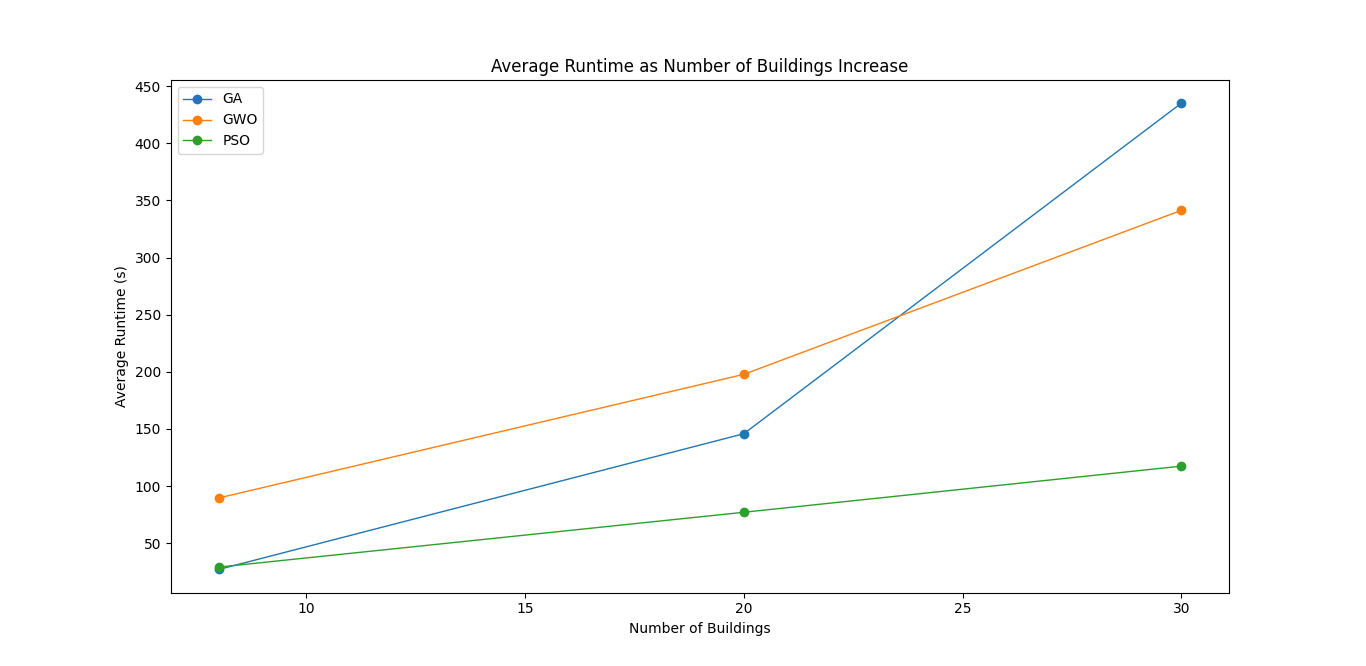
\includegraphics[scale=0.5]{./images/chap07-rd/approaches-average-runtime-over-no-of-buildings.png}
\end{adjustwidth}
\caption{The average runtime (s) of each of the approaches as the number of buildings in a data set increase.}
\label{graph-approaches-runtime-no-buildings}
\end{figure}

The genetic algorithm approach is also the fastest when SFLP-II is being used with an average run time of $27.3666666666667$s, compared to our approach's time and the PSO approach's $29.0666666666667$s. However, as the number of buildings increase, the average runtime of the GA approach becomes worse compared to the two other approaches. With mSFLP-III, GA takes $166.866666666667$s, while the PSO approach takes $223.566666666667$s and $77.0333333333333$s, respectively. GA is still faster than GWO in this data set, but it is already significantly slower than the PSO approach, unlike with the previous data set. Moving to mKra30a, we can see that GA now takes $455.5$s. This is longer than our approach, and the PSO approach's $117.4$s. Figure \ref{graph-approaches-runtime-no-buildings} shows this observation. We can attribute this faster increase in average runtime as the number of buildings increase in the GA approach to what enables it produce better solutions on average\textemdash its local search methods. Since the local search methods perform a relatively exhaustive search in order to find a better solution, the GA will take more time to finish executing. Hence, we observe this phenomenon. This is not the case with GWO and PSO, due to the lack of local search methods. GWO may have taken a longer time due to the amount of operations that are performed in the metaheuristic compared to PSO. Better implementations, especially those that utilize SIMD operations, for both approaches may reduce the gap in terms of average run time between the two. However, basing from the equations in both metaheuristics, it is likely that PSO will remain faster than GWO. Further studies, however, are required to exactly determine how well each approach scales with regards to the number of buildings.

\begin{table}[h!]
\begin{adjustwidth}{-1.15in}{}
\centering
\begin{tabular}{|l|l|l|l|l|l|}
	\hline
	\multicolumn{1}{|c|}{\multirow{2}{*}{\textbf{Problem}}} & \multicolumn{5}{c|}{\textbf{Genetic Algorithm}}                                                                                                                                                                                            \\ \cline{2-6} 
	\multicolumn{1}{|c|}{}                                  & \multicolumn{1}{c|}{\textbf{Best}} & \multicolumn{1}{c|}{\textbf{Worst}} & \multicolumn{1}{c|}{\textbf{Avg.}} & \multicolumn{1}{c|}{\textbf{Std. Dev.}} & \multicolumn{1}{c|}{\textbf{Avg. Runtime (s)}} \\ \hline
	SFLP-II                                                 & 232.839593                                  & 353.006875                                   & 274.120352366667                      &
	31.3302957404409						& 27.3666666666667                                   \\ \hline
	mSFLP-III                                               & 47177.914444                               & 53668.451469                                 & 50676.8183791                      & 1325.4427345102                                  & 166.866666666667                           \\ \hline
	mKra30a                                               & 76454.204788                                & 96215.108131                                 &
	87715.8254635							&
	4281.86238995314	                        &
	455.5								\\ \hline
\end{tabular}
\end{adjustwidth}
\caption{Results obtained from using the competing GA approach.}
\label{approach-ga-results}
\end{table}

\begin{table}[h!]
\begin{adjustwidth}{-1.18in}{}
\centering
\begin{tabular}{|l|l|l|l|l|l|}
	\hline
	\multicolumn{1}{|c|}{\multirow{2}{*}{\textbf{Problem}}} & \multicolumn{5}{c|}{\textbf{PSO}} \\ \cline{2-6} 
	\multicolumn{1}{|c|}{}                                  & \multicolumn{1}{c|}{\textbf{Best}} & \multicolumn{1}{c|}{\textbf{Worst}} & \multicolumn{1}{c|}{\textbf{Avg.}} & \multicolumn{1}{c|}{\textbf{Std. Dev.}} & \multicolumn{1}{c|}{\textbf{Avg. Runtime (s)}} \\ \hline
	SFLP-II                                                 & 273.754488                                  & 382.774055                                   &
	321.292520833333							&
	32.8103600821748							&
	29.0666666666667							\\ \hline
	mSFLP-III                                               & 59673.997963                                & 68433.641548                                 &
	64289.8051163					          &
	2356.26248290771						&
	77.0333333333333						\\ \hline
	mKra30a                                               & 107996.773666                                & 131275.843658                                 &
	121057.4221481							&
	5981.21601161922							&
	117.4						\\ \hline
\end{tabular}
\end{adjustwidth}
\caption{Results obtained from our proposed PSO approach.}
\label{approach-pso-results}
\end{table}

We can further obtain insights from our results, by looking at the best solutions generated by each approach. Figures \ref{graph-approaches-best-solutions-sflp-ii} to \ref{graph-approaches-best-solutions-mkra30a} show the fitness graphs of the best solutions using the SFLP-II, mSFLP-III, and mKra30a data sets. The non-linearity of the graph of our GWO approach that is observable in the figures is due to the nature of our approach. All solutions in a population in our approach are replaced after an iteration. Hence, the best solutions may be replaced by poorer solutions. This is unlike with the GA and PSO approaches where  the fitness continuously lower over time. In the case of the GA approach, this is due to the fact that there is elitism. The best $EN$ solutions are kept in the next generation, taking the place of the worst generated solutions produced in the current generation. The PSO approach has a similar characteristic that enables it to produce a continuously lowering fitness graph. In the PSO approach, as discussed before, each particle keeps track of the best position it has found. After an iteration, if a particle finds a position that is better than its personal best, then that position will replace the particle's personal. And if a particle's personal best is better than the swarm's global best, then that position/solution becomes the swarm's global best. It is this global best that is tracked in the graph. The selection procedure of the global best explains the graph of the PSO approach.

\begin{figure}[h!]
\centering
\begin{adjustwidth}{-0.45in}{}
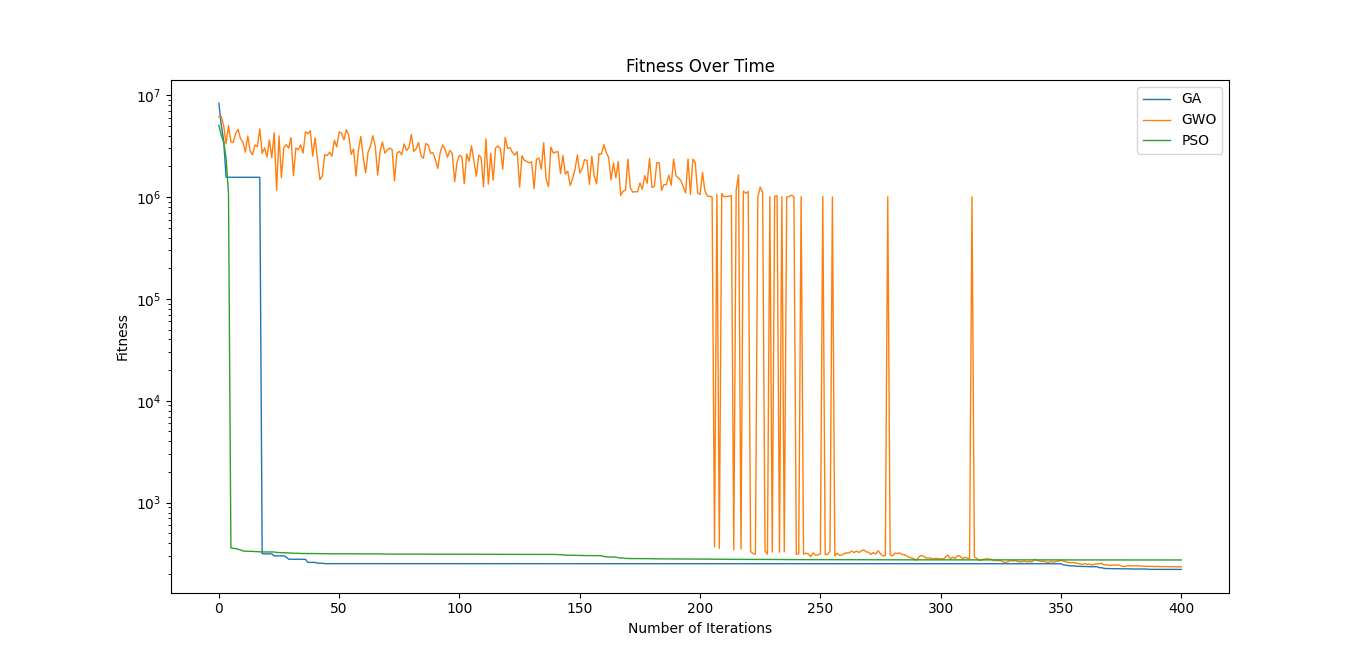
\includegraphics[scale=0.5]{./images/chap07-rd/best-fitness-over-time-sflp2.png}
\end{adjustwidth}
\caption{Fitness over time of the best solutions for the SFLP-II produced by the GA, GWO, and PSO approaches.}
\label{graph-approaches-best-solutions-sflp-ii}
\end{figure}

\begin{figure}[h!]
\centering
\begin{adjustwidth}{-0.45in}{}
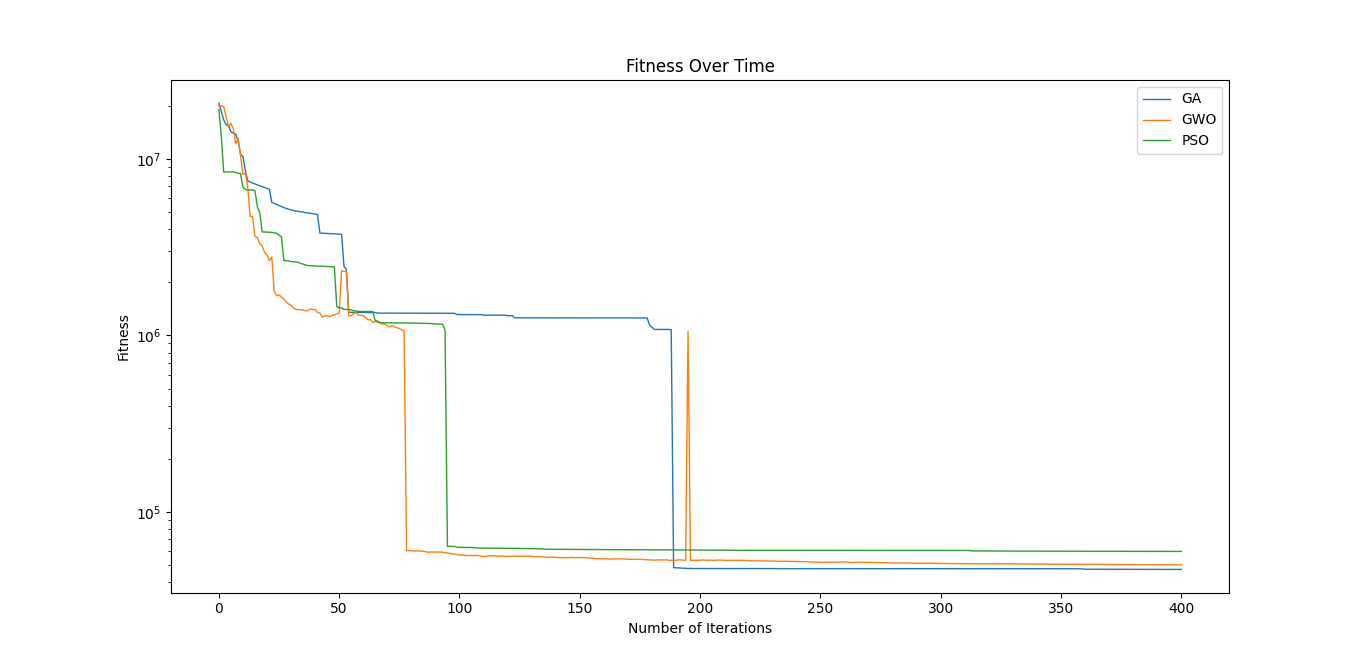
\includegraphics[scale=0.5]{./images/chap07-rd/best-fitness-over-time-msflp3.png}
\end{adjustwidth}
\caption{Fitness over time of the best solutions for the mSFLP-III produced by the GA, GWO, and PSO approaches.}
\label{graph-approaches-best-solutions-msflp-iii}
\end{figure}

\begin{figure}[h!]
\centering
\begin{adjustwidth}{-0.45in}{}
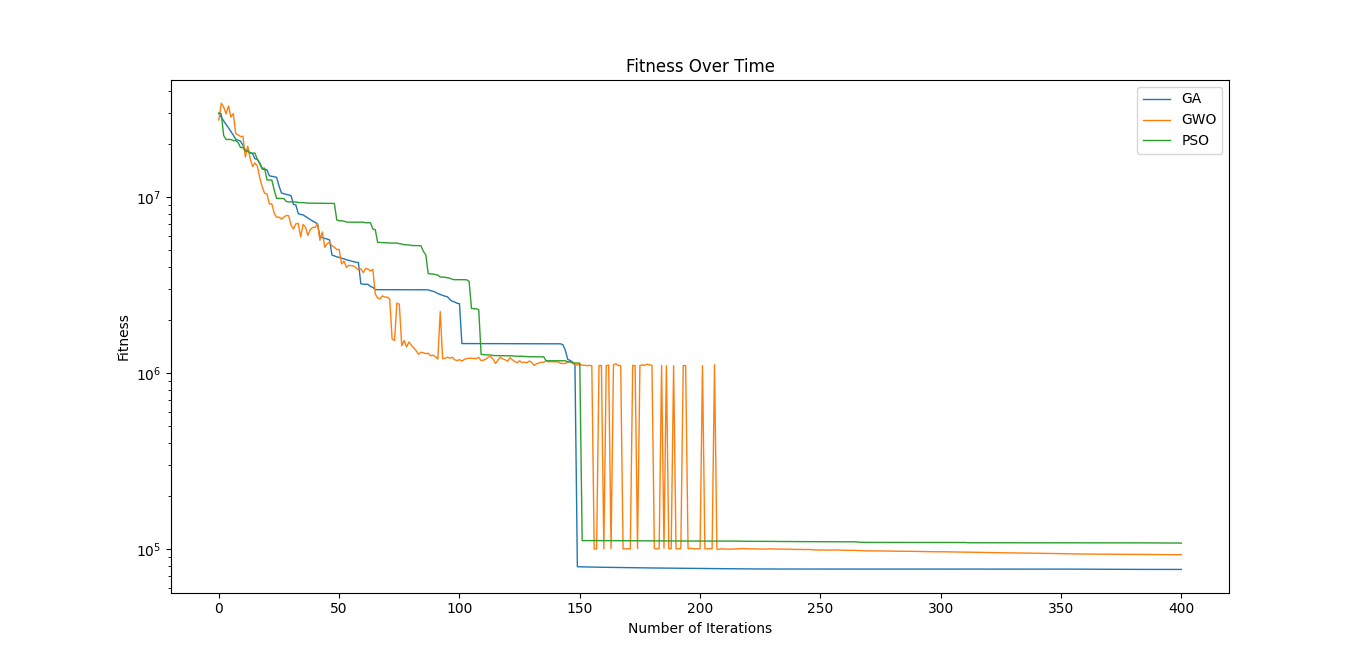
\includegraphics[scale=0.5]{./images/chap07-rd/best-fitness-over-time-mKra30a.png}
\end{adjustwidth}
\caption{Fitness over time of the best solutions for the mKra30a produced by the GA, GWO, and PSO approaches.}
\label{graph-approaches-best-solutions-mkra30a}
\end{figure}

Another avenue we can use to gather insights is through the visualization of the results produced by the approaches mentioned in this study. Figures \ref{best-results-ga} to \ref{best-results-pso} show a visualization of the best results. Notice that with the hybrid GA approach and our GWO approach, the buildings tend to clump together, which is what we want to happen, based on our objective function. For our hybrid GA approach, we can attribute the result to the local search method as well as the mutation operators as they were key to ensure that the buildings are close to each other. The crossover operator is also instrumental in achieving this result by finding combinations that will lead to the result. Our GWO approach also makes buildings clump together but not to the same degree as the GA approach, as can be observed from one building being far from the rest of the buildings in mKra30a data set in Figure \ref{best-results-gwo}. The clumping ability of our approach is attributable to how solutions are allowed to perturb their buildings to positions relatively far from the buildings positions in the best three solution initially. Eventually, our approach will decrease the distance of the buildings in a solution from the leading solutions. Remember that the leading solutions eventually become similar to each other, which help drive the reduction of the degree of building shifting. This gradually decreasing shifting of the buildings will lead to intersections from being resolved and reducing the distance of buildings from each other. The intersections are resolved by reducing the chances of buildings being to moved to a relatively further position where they would still intersect with another building, and gradually pushing intersecting buildings away from each other towards non-intersection. Note that the objective function has a lower penalty for solutions with buildings that do not significantly intersect. The decreasing shifting also encourages buildings to move towards each other due to the fact that smaller shifts have lower probability of causing buildings to intersect with one another too deeply or at all, which allows buildings to move to positions that are closer to the other buildings but without any intersections. Finally, as one can notice in Figure \ref{best-results-pso}, the PSO approach struggles to produce a solution where the buildings are clumped together. This deficiency is not necessarily clear with a small number of buildings, but it does as the number increases. We can attribute this difficulty of the PSO approach to the fact that the buildings are continuously being influenced on the same degree throughout all of the iterations by a particle's personal best and the swarm's global best. This encourages more exploitation and fewer exploitation. As a result, this reduces the chances in which buildings would be able to shift their positions by a small amount, making it more difficult for the approach to find better solutions and have buildings clump together.

\begin{figure}[h!]
\centering
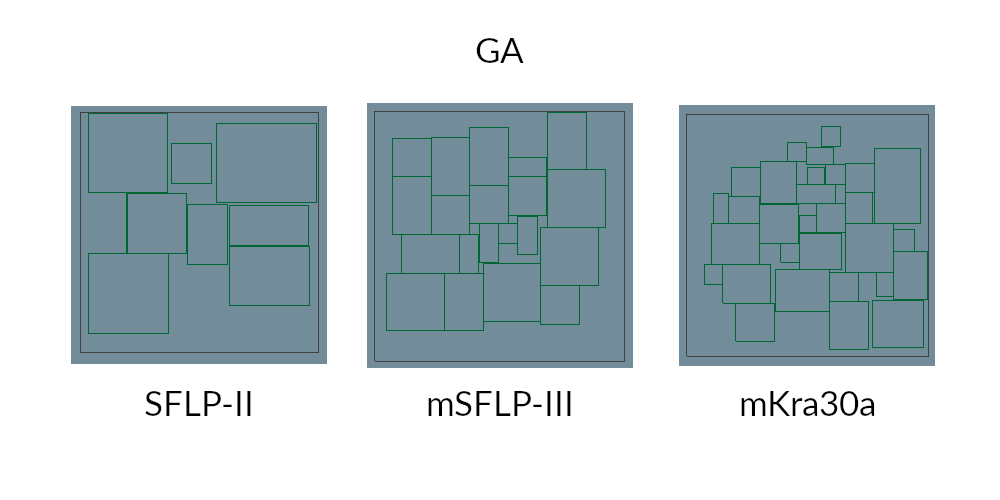
\includegraphics[scale=1.85]{./images/chap07-rd/ga-best-solutions.png}
\caption{Visualization of the best solutions produced by the hybrid GA approach for the three data sets used in this study.}
\label{best-results-ga}
\end{figure}

\begin{figure}[h!]
\centering
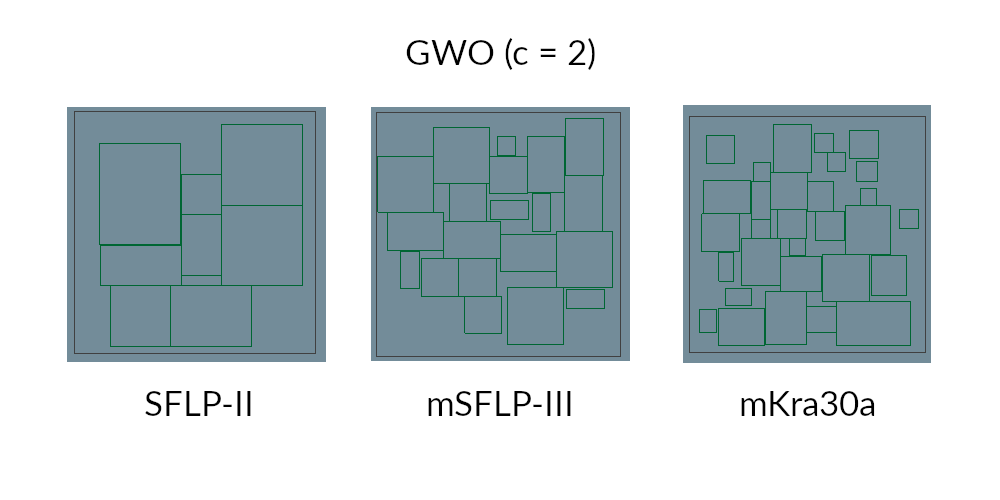
\includegraphics[scale=1.85]{./images/chap07-rd/gwo-c2-best-solutions.png}
\caption{Visualization of the best solutions produced by our GWO approach with $c=2$ for the three data sets used in this study.}
\label{best-results-gwo-c2}
\end{figure}

\begin{figure}[h!]
\centering
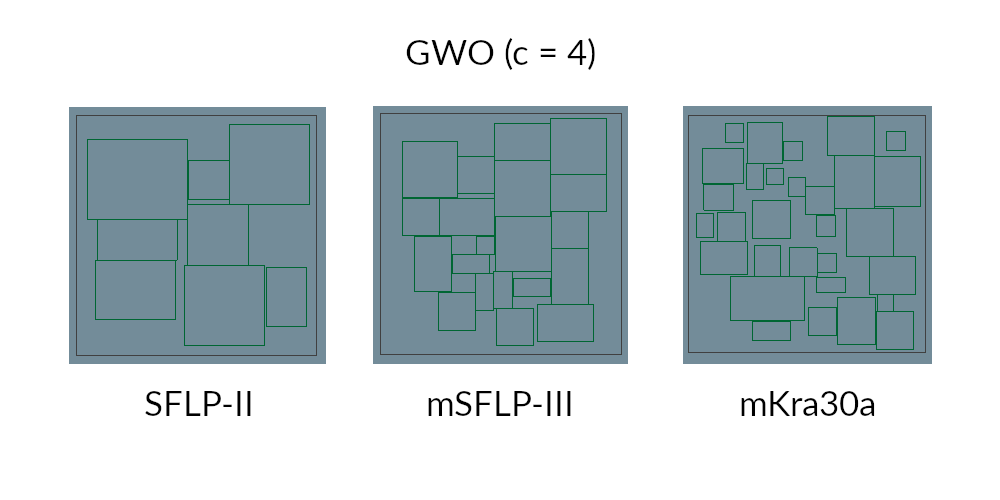
\includegraphics[scale=1.85]{./images/chap07-rd/gwo-c4-best-solutions.png}
\caption{Visualization of the best solutions produced by our GWO approach with $c=4$ for the three data sets used in this study.}
\label{best-results-gwo-c4}
\end{figure}

\begin{figure}[h!]
\centering
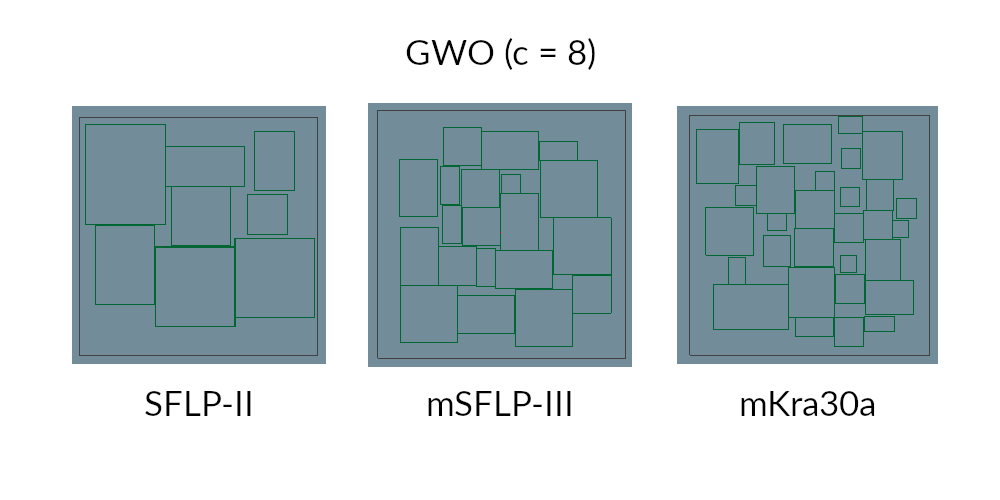
\includegraphics[scale=1.85]{./images/chap07-rd/gwo-c8-best-solutions.png}
\caption{Visualization of the best solutions produced by our GWO approach with $c=12$ for the three data sets used in this study.}
\label{best-results-gwo-c8}
\end{figure}

\begin{figure}[h!]
\centering
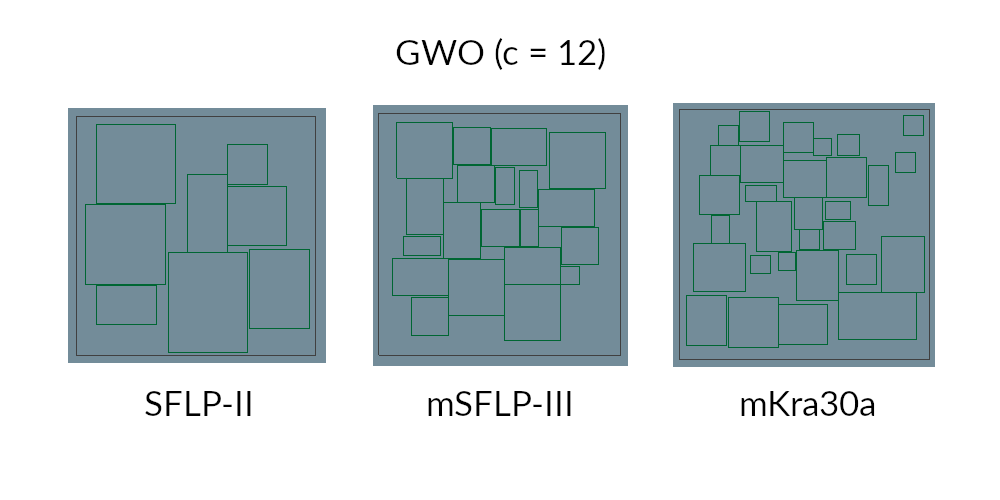
\includegraphics[scale=1.85]{./images/chap07-rd/gwo-c12-best-solutions.png}
\caption{Visualization of the best solutions produced by our GWO approach with $c=12$ for the three data sets used in this study.}
\label{best-results-gwo}
\end{figure}

\begin{figure}[h!]
\centering
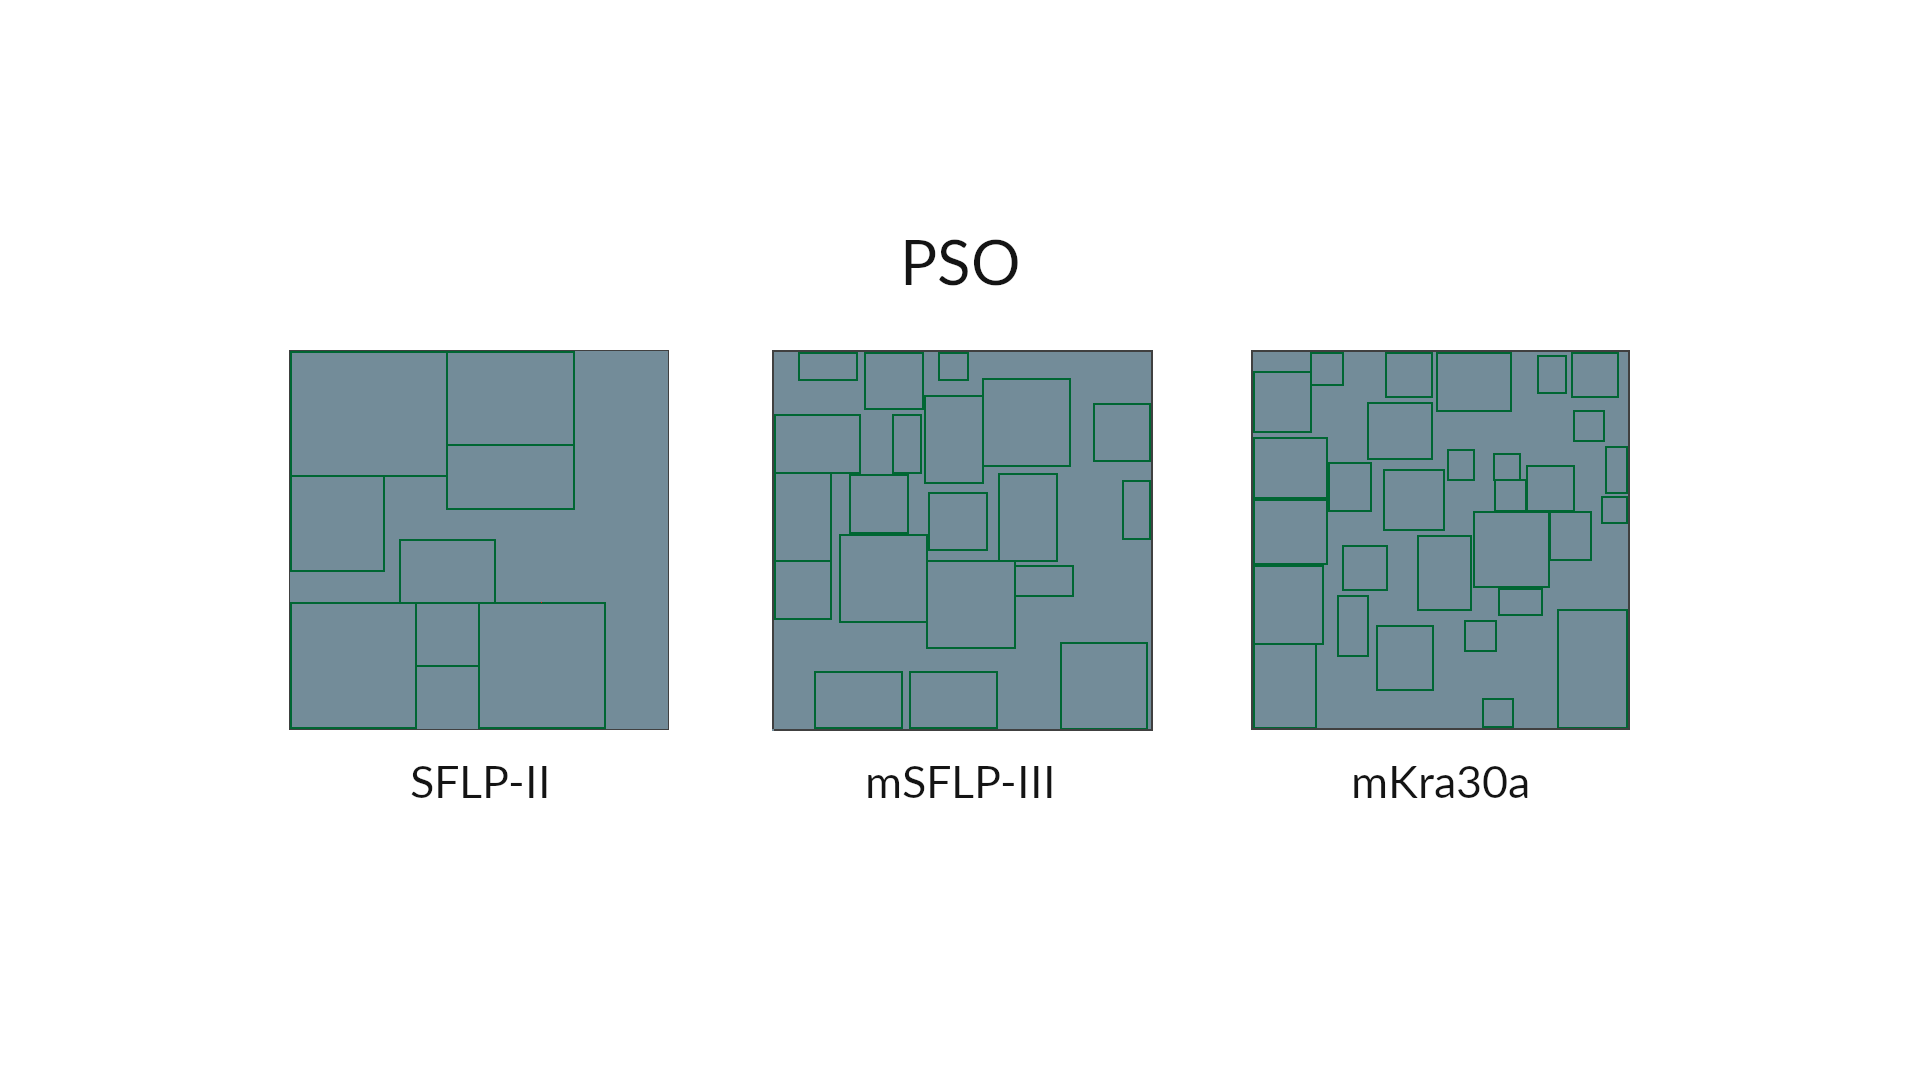
\includegraphics[scale=1.85]{./images/chap07-rd/pso-best-solutions.png}
\caption{Visualization of the best solutions produced by the PSO approach for the three data sets used in this study.}
\label{best-results-pso}
\end{figure}

For reference, Tables \ref{full-data-ga} to \ref{full-data-pso} provide the detailed numbers we have obtained in our experiments for each approach and data set. Table \ref{full-data-ga} shows the entire experiment data for our hybrid GA approach, table \ref{full-data-gwo} shows the data for our GWO approach, and lastly, table \ref{full-data-pso} shows the data for the PSO approach.

\begin{table}
\centering
\begin{adjustwidth}{}{}
\resizebox{\textwidth}{!}{\rotatebox{90}{
\begin{tabular}{|r|r|r|r|r|r|r|} 
\hline
\multicolumn{1}{|c|}{\multirow{2}{*}{Run}} & \multicolumn{6}{c|}{GA Experimental Results}                                                                                                                                                                          \\ 
\cline{2-7}
\multicolumn{1}{|c|}{}                     & \multicolumn{1}{l|}{SFLP-II} & \multicolumn{1}{l|}{Elapsed Time (s)} & \multicolumn{1}{l|}{mSFLP-III} & \multicolumn{1}{l|}{Elapsed Time (s)} & \multicolumn{1}{l|}{mKra30a} & \multicolumn{1}{l|}{Elapsed Time (s)}  \\ 
\hline
1                                          & 241.353251                   & 31                                    & 51469.406654                   & 155                                   & 76454.204788                 & 417                                    \\ 
\hline
2                                          & 260.666385                   & 27                                    & 50203.262684                   & 166                                   & 90215.278652                 & 454                                    \\ 
\hline
3                                          & 317.934947                   & 34                                    & 49903.403969                   & 159                                   & 80078.077255                 & 442                                    \\ 
\hline
4                                          & 257.12075                    & 26                                    & 51214.094765                   & 149                                   & 85424.753021                 & 453                                    \\ 
\hline
5                                          & 252.747648                   & 26                                    & 49754.550606                   & 152                                   & 85276.805458                 & 416                                    \\ 
\hline
6                                          & 291.574655                   & 27                                    & 49526.201752                   & 160                                   & 88156.523018                 & 472                                    \\ 
\hline
7                                          & 292.021864                   & 27                                    & 49669.613991                   & 157                                   & 83149.07745                  & 423                                    \\ 
\hline
8                                          & 281.474234                   & 27                                    & 51731.675354                   & 176                                   & 88411.142647                 & 413                                    \\ 
\hline
9                                          & 269.290927                   & 26                                    & 51245.732857                   & 172                                   & 90734.373741                 & 478                                    \\ 
\hline
10                                         & 269.423721                   & 27                                    & 48920.435341                   & 175                                   & 87220.602196                 & 488                                    \\ 
\hline
11                                         & 240.832309                   & 26                                    & 52856.025909                   & 212                                   & 81419.135918                 & 446                                    \\ 
\hline
12                                         & 259.251911                   & 24                                    & 49490.654926                   & 144                                   & 89084.201248                 & 498                                    \\ 
\hline
13                                         & 257.123175                   & 27                                    & 51225.387764                   & 164                                   & 82219.564217                 & 449                                    \\ 
\hline
14                                         & 232.839593                   & 26                                    & 49141.684452                   & 197                                   & 91560.704735                 & 440                                    \\ 
\hline
15                                         & 305.979567                   & 27                                    & 52062.448891                   & 161                                   & 85431.277306                 & 446                                    \\ 
\hline
16                                         & 263.951872                   & 26                                    & 51269.011093                   & 175                                   & 93689.351776                 & 451                                    \\ 
\hline
17                                         & 271.432117                   & 25                                    & 52881.041428                   & 176                                   & 85395.590744                 & 431                                    \\ 
\hline
18                                         & 278.044098                   & 33                                    & 51087.689514                   & 180                                   & 87894.849144                 & 421                                    \\ 
\hline
19                                         & 266.951438                   & 28                                    & 51001.627296                   & 171                                   & 91152.267059                 & 445                                    \\ 
\hline
20                                         & 246.816533                   & 27                                    & 50198.549866                   & 178                                   & 88895.677979                 & 471                                    \\ 
\hline
21                                         & 275.481676                   & 27                                    & 50003.058311                   & 162                                   & 87140.735931                 & 468                                    \\ 
\hline
22                                         & 353.006875                   & 26                                    & 51480.186226                   & 162                                   & 88911.361496                 & 533                                    \\ 
\hline
23                                         & 336.045243                   & 26                                    & 51068.014679                   & 182                                   & 88503.003464                 & 499                                    \\ 
\hline
24                                         & 267.427919                   & 28                                    & 53668.451469                   & 177                                   & 90751.106781                 & 487                                    \\ 
\hline
25                                         & 318.71513                    & 28                                    & 49688.022858                   & 167                                   & 87554.161316                 & 480                                    \\ 
\hline
26                                         & 239.385818                   & 31                                    & 50890.728996                   & 161                                   & 89753.353699                 & 516                                    \\ 
\hline
27                                         & 235.181557                   & 27                                    & 51466.78817                    & 160                                   & 92770.250797                 & 431                                    \\ 
\hline
28                                         & 256.815948                   & 27                                    & 47177.914444                   & 159                                   & 93206.425659                 & 443                                    \\ 
\hline
29                                         & 329.646141                   & 27                                    & 50171.089684                   & 146                                   & 84805.798279                 & 473                                    \\ 
\hline
30                                         & 255.073269                   & 27                                    & 49837.797424                   & 151                                   & 96215.108131                 & 381                                    \\ 
\hline
\multicolumn{1}{|l|}{Average}              & 274.120352366667             & 27.3666666666667                      & 50676.8183791                  & 166.866666666667                      & 87715.8254635                & 455.5                                  \\ 
\hline
\multicolumn{1}{|l|}{Std. Dev}             & 31.3302957404409             & 2.17324377503931                      & 1325.4427345102                & 14.6775299372024                      & 4281.86238995314             & 33.3639801644497                       \\
\hline
\end{tabular}}}
\end{adjustwidth}
\caption{The entire experiment data we have collected using our hybrid GA approach.}
\label{full-data-ga}
\end{table}

\begin{table}
\centering
\begin{adjustwidth}{}{}
\resizebox{\textwidth}{!}{\rotatebox{90}{
\begin{tabular}{|r|r|r|r|r|r|r|} 
\hline
\multicolumn{1}{|c|}{\multirow{2}{*}{Run}} & \multicolumn{6}{c|}{PSO Experimental Results}                                                                                                                                                                         \\ 
\cline{2-7}
\multicolumn{1}{|c|}{}                     & \multicolumn{1}{l|}{SFLP-II} & \multicolumn{1}{l|}{Elapsed Time (s)} & \multicolumn{1}{l|}{mSFLP-III} & \multicolumn{1}{l|}{Elapsed Time (s)} & \multicolumn{1}{l|}{mKra30a} & \multicolumn{1}{l|}{Elapsed Time (s)}  \\ 
\hline
1                                          & 318.852793                   & 30                                    & 64984.15004                    & 76                                    & 126400.957298                & 130                                    \\ 
\hline
2                                          & 322.977083                   & 28                                    & 65613.267347                   & 81                                    & 121843.241837                & 115                                    \\ 
\hline
3                                          & 319.688772                   & 27                                    & 66182.148331                   & 77                                    & 131064.62114                 & 117                                    \\ 
\hline
4                                          & 382.774055                   & 29                                    & 65321.947243                   & 74                                    & 123193.080185                & 109                                    \\ 
\hline
5                                          & 328.181972                   & 26                                    & 68316.333054                   & 90                                    & 113509.606079                & 116                                    \\ 
\hline
6                                          & 273.754488                   & 27                                    & 63051.351074                   & 80                                    & 126382.984985                & 104                                    \\ 
\hline
7                                          & 277.929458                   & 35                                    & 64844.383484                   & 80                                    & 118793.658676                & 113                                    \\ 
\hline
8                                          & 333.791855                   & 29                                    & 62119.790359                   & 78                                    & 116690.745407                & 115                                    \\ 
\hline
9                                          & 331.588456                   & 25                                    & 62520.697372                   & 81                                    & 112328.409836                & 114                                    \\ 
\hline
10                                         & 312.062043                   & 28                                    & 60370.992424                   & 70                                    & 125547.949913                & 117                                    \\ 
\hline
11                                         & 347.300041                   & 26                                    & 63191.887421                   & 74                                    & 128467.742325                & 111                                    \\ 
\hline
12                                         & 276.72711                    & 29                                    & 66079.518539                   & 75                                    & 115259.262817                & 123                                    \\ 
\hline
13                                         & 346.501261                   & 38                                    & 68433.641548                   & 72                                    & 120682.394836                & 123                                    \\ 
\hline
14                                         & 324.057936                   & 29                                    & 59673.997963                   & 73                                    & 115606.839714                & 136                                    \\ 
\hline
15                                         & 294.477526                   & 33                                    & 65232.604935                   & 77                                    & 107996.773666                & 135                                    \\ 
\hline
16                                         & 354.944439                   & 28                                    & 62623.302681                   & 77                                    & 117466.287628                & 119                                    \\ 
\hline
17                                         & 278.580433                   & 25                                    & 63571.512451                   & 78                                    & 119787.763885                & 111                                    \\ 
\hline
18                                         & 373.62812                    & 25                                    & 65604.954414                   & 73                                    & 121933.62674                 & 111                                    \\ 
\hline
19                                         & 277.326199                   & 27                                    & 60121.135582                   & 71                                    & 120619.96003                 & 128                                    \\ 
\hline
20                                         & 312.888415                   & 26                                    & 65799.8442                     & 77                                    & 114528.809418                & 112                                    \\ 
\hline
21                                         & 349.500618                   & 28                                    & 62835.800159                   & 86                                    & 123371.321442                & 113                                    \\ 
\hline
22                                         & 324.432381                   & 30                                    & 67968.856182                   & 80                                    & 125755.185791                & 107                                    \\ 
\hline
23                                         & 259.640869                   & 29                                    & 61263.364929                   & 77                                    & 114837.336021                & 109                                    \\ 
\hline
24                                         & 324.809072                   & 28                                    & 64277.566399                   & 78                                    & 119911.446892                & 114                                    \\ 
\hline
25                                         & 315.892269                   & 30                                    & 63997.453415                   & 72                                    & 130395.024284                & 101                                    \\ 
\hline
26                                         & 367.985685                   & 31                                    & 62791.55909                    & 73                                    & 126777.9534                  & 109                                    \\ 
\hline
27                                         & 306.720735                   & 37                                    & 66069.317642                   & 77                                    & 116590.569717                & 132                                    \\ 
\hline
28                                         & 373.704857                   & 29                                    & 65694.84201                    & 77                                    & 131275.843658                & 145                                    \\ 
\hline
29                                         & 288.776388                   & 30                                    & 67406.459572                   & 76                                    & 118132.533211                & 120                                    \\ 
\hline
30                                         & 339.280296                   & 30                                    & 62731.473629                   & 81                                    & 126570.733612                & 113                                    \\ 
\hline
\multicolumn{1}{|l|}{Average}              & 321.292520833333             & 29.0666666666667                      & 64289.8051163                  & 77.0333333333333                      & 121057.4221481               & 117.4                                  \\ 
\hline
\multicolumn{1}{|l|}{Std. Dev}             & 32.8103600821748             & 3.20488133443597                      & 2356.26248290771               & 4.29501180868943                      & 5981.21601161922             & 10.1526283330459                       \\
\hline
\end{tabular}}}
\end{adjustwidth}
\caption{The entire experiment data we have collected using our PSO approach.}
\label{full-data-pso}
\end{table}

The performance of the GA approach in this study is definitely noteworthy. It produces the best solutions on average among the three approaches. However, based on the results, the GA approach does not scale well as the number of buildings increase, compared to our approach and the PSO approach. PSO definitely shows the best average runtimes. However, it produces the worst average fitness. For faster speed, we traded performance. This is where our approach shines. Our approach is the second best when it comes to solution quality as the problem scales higher. It is also the second best in terms of speed. This shows to us that our GWO approach provides a balance between speed and performance. Our approach also requires only a few parameters. We argue that this will simplify and speed up experimental setups and configuration in later studies and applications. Importantly, the results also indicate that there is promise in further exploring the applicability of the grey wolf optimization algorithm in solving the facility layout problem.

\chapter{Conclusion and Summary}

In this study, we proposed an alternative approach to the static unequal area facility layout problem, which was previously solved using genetic algorithm and particle swarm optimization. Our alternative approach utilizes the grey wolf optimization to solve the problem. We have introduced modifications to this metaheuristic in order for it to be able to produce feasible solutions. We have compared this modified GWO against a GA-based hybrid approach. Results from our experiment indicate that the GA-based approach is generally than our modified GWO. However, they showed that there is promise in GWO as an algorithm for solving FLPs. In one data set, our approach produced results faster than the GA-based approach, despite producing an average result that is slightly worse than the other approach. Our approach is also simpler, making it easier to understand and experiment with. In the future, our proposed modified GWO may be further improved to produce significantly better results. Besides, GWO is relatively new to the field, providing researchers with plentiful opportunities to improve the algorithm. Modifying the equations of our modified GWO, such as the decay rate of $\alpha$, is one avenue in which researchers may take to build upon our study.

\appendix

\chapter{What should be in the Appendix}

What goes in the appendices? Any material which impedes the smooth
development of your presentation, but which is important to justify the
results of a thesis. Generally it is material that is of too nitty-gritty
a level of detail for inclusion in the main body of the thesis, but which
should be available for perusal by the examiners to convince them
sufficiently. Examples include program listings, immense tables of data,
lengthy mathematical proofs or derivations, etc.



% ------------------------------------------------------------------------
\INPUT{biblio.bib} 
\setlinespacing{1.44}
\bibliographystyle{plain}
\bibliography{biblio}
\end{document}
% ------------------------------------------------------------------------
